% Presentazione revisionata: Introduzione a R e all'analisi dei dati
% Basata sul materiale originale fornito dall'autore e sul template M01_Pensare_con_i_dati.tex
% Compilazione: xelatex -interaction=nonstopmode R_analisi_dati_completa.tex (due passaggi)
% Le figure vettoriali sono contenute in Risorse/Figure/.
% Revisione completa delle 85 slide; fonti consultate il 18 novembre 2026.
\documentclass[12pt,aspectratio=1610]{beamer}
\geometry{paperwidth=20cm,paperheight=12.5cm}
\usepackage[italian,provide=*]{babel}
\usepackage{fontspec}
\IfFontExistsTF{NimbusSans-Regular.otf}{
\setsansfont{NimbusSans-Regular.otf}[BoldFont=NimbusSans-Bold.otf,ItalicFont=NimbusSans-Italic.otf,BoldItalicFont=NimbusSans-BoldItalic.otf]
\setmainfont{NimbusSans-Regular.otf}[BoldFont=NimbusSans-Bold.otf,ItalicFont=NimbusSans-Italic.otf,BoldItalicFont=NimbusSans-BoldItalic.otf]
}{
\setsansfont{TeX Gyre Heros}
\setmainfont{TeX Gyre Heros}
}
\IfFontExistsTF{DejaVu Sans Mono}{
\setmonofont{DejaVu Sans Mono}[Scale=.88]
}{\setmonofont{Latin Modern Mono}[Scale=.88]}
\usefonttheme{professionalfonts}
\usepackage{amsmath,amssymb,booktabs,array,graphicx,tikz,bookmark}
\usetikzlibrary{calc,positioning,arrows.meta}
\graphicspath{{Risorse/Figure/}}
\definecolor{Paper}{HTML}{F8F6F1}
\definecolor{Ink}{HTML}{253344}
\definecolor{Navy}{HTML}{15283E}
\definecolor{Quantum}{HTML}{5146A5}
\definecolor{Classical}{HTML}{087C74}
\definecolor{Muted}{HTML}{657180}
\definecolor{Rule}{HTML}{D6DAD9}
\definecolor{Night}{HTML}{112236}
\definecolor{Lilac}{HTML}{ABB5FF}
\definecolor{Mint}{HTML}{72D8C8}
\setbeamercolor{background canvas}{bg=Paper}
\setbeamercolor{normal text}{fg=Ink}
\setbeamertemplate{navigation symbols}{}
\setbeamertemplate{headline}{}
\setbeamertemplate{footline}{}
\setbeamersize{text margin left=0pt,text margin right=0pt}
\hypersetup{colorlinks=true,linkcolor=Classical,urlcolor=Classical,pdfpagemode=UseOutlines,pdfstartview=Fit,
 pdftitle={Introduzione a R e all'analisi dei dati},pdfauthor={Marzio De Corato},
 pdfsubject={Lezione su R e analisi dati, Revisione completa: diagrammi TikZ, formule e codice R commentato}}
\bookmarksetup{open,openlevel=0,depth=2}
\newsavebox{\BodyBox}
\newsavebox{\SideBox}
\newsavebox{\RecallBox}
\newsavebox{\TitleBox}
\newcommand{\MeasureBox}[2]{\typeout{REVIEWBOX:#1:\the\wd#2:\the\ht#2:\the\dp#2}}

% Revisione completa: diagrammi TikZ, formalismo e box R.
\usepackage[most]{tcolorbox}
\usepackage{listings}
\usetikzlibrary{fit,backgrounds,matrix,decorations.pathreplacing}
\definecolor{GeoA}{HTML}{1D7890}
\definecolor{GeoB}{HTML}{C57E42}
\definecolor{GeoC}{HTML}{7363AA}
\definecolor{GeoTint}{HTML}{F0F4F3}
\lstdefinestyle{GeoR}{language=R,basicstyle=\ttfamily\fontsize{9.2}{12.2}\selectfont,
 keywordstyle=\color{Quantum}\bfseries,commentstyle=\color{Classical},stringstyle=\color{GeoB},
 numbers=left,numberstyle=\tiny\color{Muted},numbersep=4pt,showstringspaces=false,
 columns=fullflexible,keepspaces=true,breaklines=true,xleftmargin=1.15em,
 frame=none,aboveskip=0pt,belowskip=0pt,tabsize=2}
\newsavebox{\PilotLeftBox}
\newsavebox{\PilotRightBox}
\newcommand{\PLabel}[1]{\par{\color{Classical}\bfseries\fontsize{9}{11}\selectfont\MakeUppercase{#1}}\par\vspace{1.8mm}}
\newcommand{\PBody}[1]{\par{\fontsize{11.3}{14.8}\selectfont #1\par}}
\newcommand{\PSmall}[1]{\par{\fontsize{9.8}{13.1}\selectfont #1\par}}
\newcommand{\PCode}[2]{%
\begin{tcolorbox}[enhanced,arc=1.8mm,boxrule=.65pt,
  colback=white,colframe=Classical!75!Navy,colbacktitle=Navy,
  coltitle=white,fonttitle=\bfseries\fontsize{9.6}{12}\selectfont,
  title={#1},left=1.7mm,right=1.3mm,top=1.5mm,bottom=1.3mm,
  before skip=1mm,after skip=1mm]
\lstinputlisting[style=GeoR]{Codice/#2}
\end{tcolorbox}}
\newcommand{\PInfo}[1]{%
\begin{tcolorbox}[enhanced,arc=1.6mm,boxrule=.55pt,colback=GeoTint,
 colframe=Rule!80!Classical,left=2.3mm,right=2.3mm,top=2mm,bottom=2mm,
 before skip=1mm,after skip=1mm]
\PSmall{#1}\end{tcolorbox}}
\tikzset{
 pFlow/.style={draw=Classical!45,fill=white,rounded corners=2mm,
  line width=.7pt,align=center,minimum height=1.1cm,font=\sffamily\fontsize{10}{12}\selectfont},
 pEdge/.style={-{Latex[length=2.3mm]},draw=Classical,line width=.95pt},
 pGroup/.style={draw=Rule,fill=white,rounded corners=2mm,line width=.65pt},
 pDotA/.style={circle,fill=GeoA,inner sep=1.25pt},
 pDotB/.style={circle,fill=GeoB,inner sep=1.25pt},
 pDotC/.style={circle,fill=GeoC,inner sep=1.25pt}
}
\newcommand{\PilotChrome}[4]{%
  \node[anchor=north west,inner sep=0,text width=17.7cm] at ([xshift=.95cm,yshift=-.55cm]current page.north west) {\color{Navy}\bfseries\fontsize{20.6}{24.5}\selectfont #1};
  \node[anchor=north east,inner sep=0] at ([xshift=19.05cm,yshift=-.14cm]current page.north west) {\color{Classical}\fontsize{8}{10}\selectfont\hyperlink{slide2}{#2}};
  \draw[Classical,line width=1.2pt] ([xshift=.95cm,yshift=-1.7cm]current page.north west)--([xshift=2.35cm,yshift=-1.7cm]current page.north west);
  \draw[Rule,line width=.65pt] ([xshift=.95cm,yshift=-10.36cm]current page.north west)--([xshift=19.05cm,yshift=-10.36cm]current page.north west);
  \node[anchor=north west,inner sep=0] at ([xshift=.96cm,yshift=-10.55cm]current page.north west) {\color{Classical}\bfseries\fontsize{9.1}{12}\selectfont DA RICORDARE};
  \node[anchor=north west,inner sep=0,text width=14.3cm] at ([xshift=4.2cm,yshift=-10.53cm]current page.north west) {\color{Ink}\fontsize{10.3}{13.8}\selectfont #4};
  \draw[Rule,line width=.35pt] ([xshift=.95cm,yshift=-11.92cm]current page.north west)--([xshift=19.05cm,yshift=-11.92cm]current page.north west);
  \node[anchor=north west,inner sep=0] at ([xshift=.95cm,yshift=-12.06cm]current page.north west) {\color{Muted}\fontsize{7.7}{9.2}\selectfont Introduzione a R e all'analisi dei dati};
  \node[anchor=north east,inner sep=0] at ([xshift=19.05cm,yshift=-12.06cm]current page.north west) {\color{Muted}\fontsize{7.7}{9.2}\selectfont #3/84};
}


% Stili comuni per i diagrammi scientifici della revisione completa.
\tikzset{
 pAxis/.style={-{Latex[length=2mm]},draw=Muted,line width=.65pt},
 pNote/.style={font=\sffamily\fontsize{9}{11.5}\selectfont,text=Muted,align=center},
 pLabel/.style={font=\sffamily\fontsize{10}{12.5}\selectfont,text=Ink,align=center}
}
\newsavebox{\FullWideBox}
\setlength{\emergencystretch}{1em}

\begin{document}

\begin{frame}[plain]\hypertarget{slide1}{}
% Copertina 3D: immagine renderizzata in Blender e titoli LaTeX sovrapposti.
\begin{tikzpicture}[remember picture,overlay]
\fill[Night] (current page.south west) rectangle (current page.north east);
\node[anchor=south west,inner sep=0,outer sep=0] at (current page.south west) {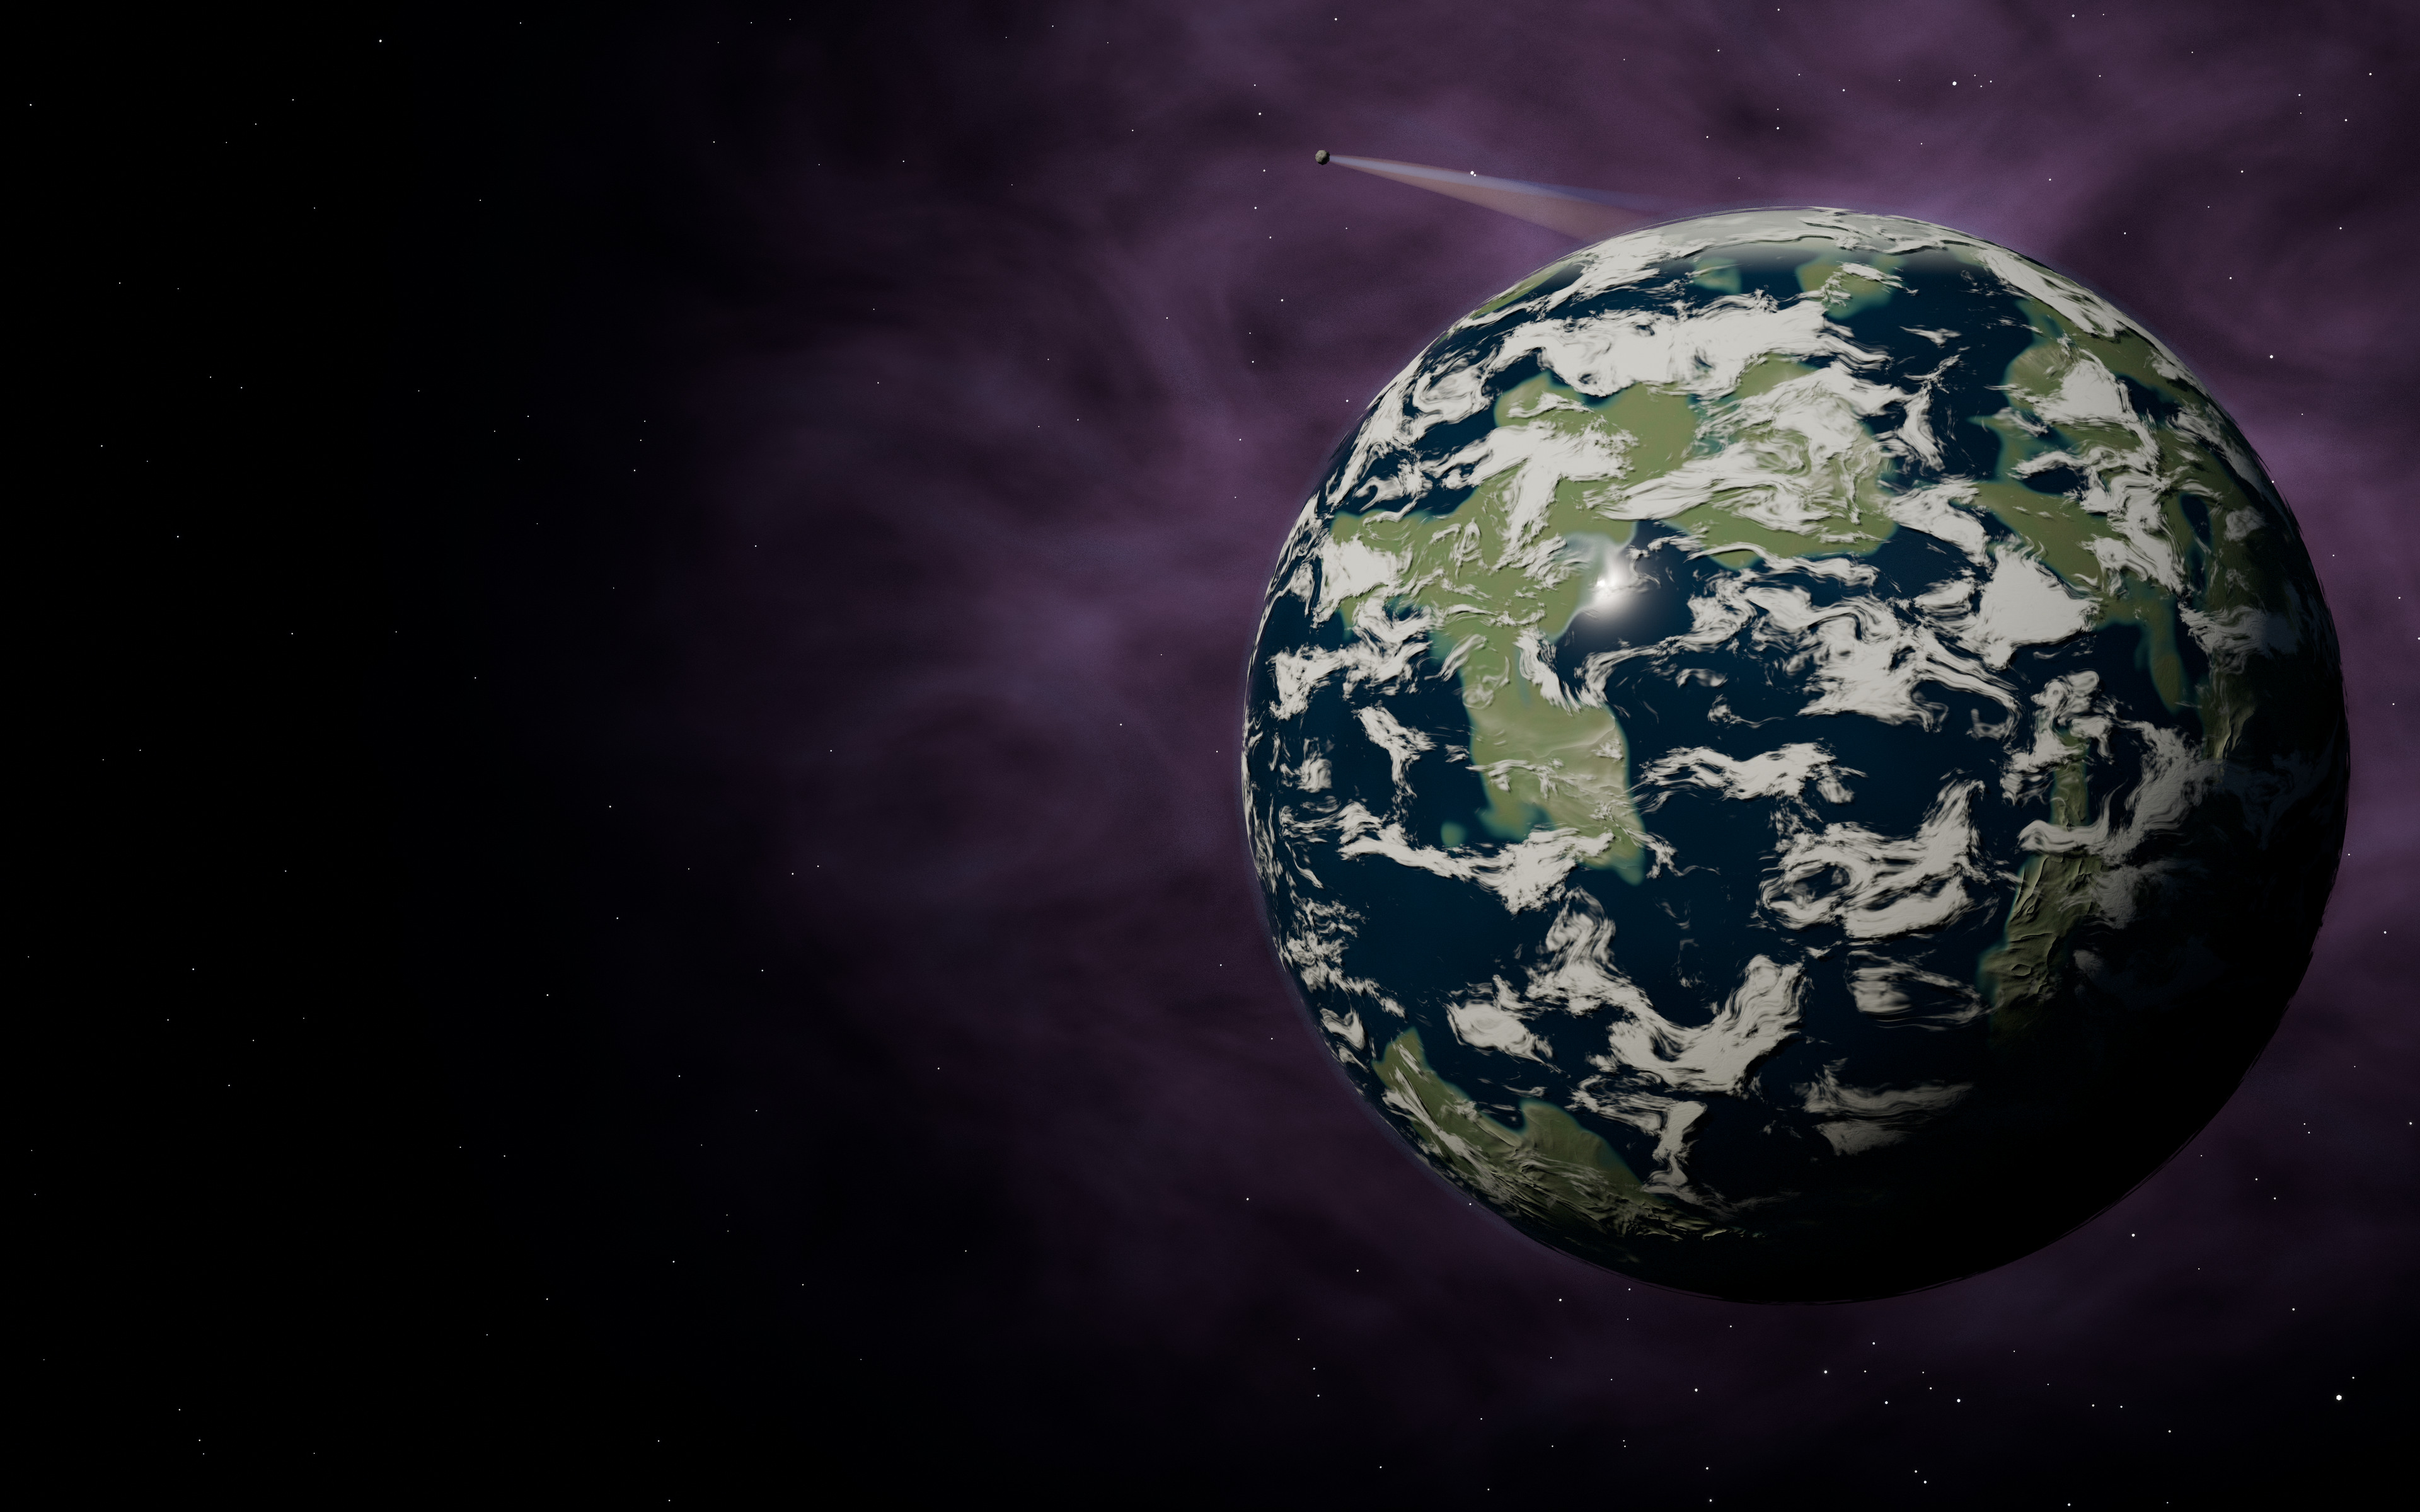
\includegraphics[width=\paperwidth,height=\paperheight]{Risorse/Copertine/M01_Terra.jpg}};

\node[anchor=north west,inner sep=0,text width=9.2cm] at
 ([xshift=1.05cm,yshift=-1.10cm]current page.north west)
 {\color{Mint}\bfseries\fontsize{23}{27}\selectfont TERRA};
\node[anchor=north west,inner sep=0,text width=9.2cm] at
 ([xshift=1.07cm,yshift=-2.16cm]current page.north west)
 {\color{white}\fontsize{9.0}{12}\selectfont MODULO M01 · SCIENZE DELLA TERRA};
\draw[Mint,line width=1.4pt] ([xshift=1.05cm,yshift=-2.78cm]current page.north west)--
 ([xshift=2.60cm,yshift=-2.78cm]current page.north west);
\node[anchor=north west,inner sep=0] at
 ([xshift=1.05cm,yshift=-3.35cm]current page.north west)
 {\begin{minipage}{9.2cm}\raggedright\color{white}\bfseries
 \fontsize{30}{36}\selectfont Introduzione a R\\e all’analisi\\dei dati\end{minipage}};
\node[anchor=north west,inner sep=0] at
 ([xshift=1.07cm,yshift=-7.88cm]current page.north west)
 {\begin{minipage}{9.0cm}\raggedright\color{Lilac}
 \fontsize{12.2}{17}\selectfont Fondamenti di R e analisi quantitativa\\nelle scienze della Terra\end{minipage}};
\node[anchor=north west,inner sep=0,text width=9.2cm] at
 ([xshift=1.07cm,yshift=-10.52cm]current page.north west)
 {\color{white}\fontsize{11.5}{15}\selectfont Marzio De Corato};
\node[anchor=north west,inner sep=0,text width=9.2cm] at
 ([xshift=1.07cm,yshift=-11.17cm]current page.north west)
 {\color{Lilac}\fontsize{8.8}{11}\selectfont \href{https://creativecommons.org/licenses/by-nc-sa/4.0/}{\textcopyright{} 2026 · CC BY-NC-SA 4.0}};
\end{tikzpicture}
\end{frame}


\begin{frame}[plain]\hypertarget{slide2}{}
\bookmark[level=0,page=2]{Domanda centrale}
\begin{tikzpicture}[remember picture,overlay]
\node[anchor=north west,inner sep=0] at ([xshift=.95cm,yshift=-.67cm]current page.north west) {\color{Navy}\bfseries\fontsize{23}{27}\selectfont Dai dati alla domanda scientifica};
\draw[Classical,line width=1.4pt] ([xshift=.95cm,yshift=-1.73cm]current page.north west)--([xshift=2.5cm,yshift=-1.73cm]current page.north west);
\node[anchor=north west,inner sep=0,fill=GeoTint,rounded corners=2mm,text width=17.7cm,inner sep=3.5mm] at ([xshift=1.0cm,yshift=-2.26cm]current page.north west) {\color{Navy}\fontsize{14.1}{19}\selectfont Quale grandezza osserviamo, su quali unità e per quale popolazione?};
\node[draw=Rule,line width=.7pt,fill=GeoTint,rounded corners=2.5mm,minimum width=4.8cm,minimum height=2.15cm,text width=4.38cm,align=center,inner sep=3mm] (n0) at ([xshift=4cm,yshift=-6.15cm]current page.north west) {\color{Navy}\bfseries\fontsize{13}{16}\selectfont MISURA\\[2mm]\color{Ink}\normalfont\fontsize{10.5}{14}\selectfont Valori e unità fisiche};
\node[draw=Rule,line width=.7pt,fill=Paper,rounded corners=2.5mm,minimum width=4.8cm,minimum height=2.15cm,text width=4.38cm,align=center,inner sep=3mm] (n1) at ([xshift=10cm,yshift=-6.15cm]current page.north west) {\color{Navy}\bfseries\fontsize{13}{16}\selectfont DISEGNO\\[2mm]\color{Ink}\normalfont\fontsize{10.5}{14}\selectfont Provini e stazioni\\nel dominio};
\node[draw=Rule,line width=.7pt,fill=GeoTint,rounded corners=2.5mm,minimum width=4.8cm,minimum height=2.15cm,text width=4.38cm,align=center,inner sep=3mm] (n2) at ([xshift=16cm,yshift=-6.15cm]current page.north west) {\color{Navy}\bfseries\fontsize{13}{16}\selectfont CONCLUSIONE\\[2mm]\color{Ink}\normalfont\fontsize{10.5}{14}\selectfont Quantità e limiti espliciti};
\draw[-{Stealth[length=3.0mm]},draw=Classical,line width=1.45pt] ([xshift=6.65cm,yshift=-6.15cm]current page.north west)--([xshift=7.35cm,yshift=-6.15cm]current page.north west);
\draw[-{Stealth[length=3.0mm]},draw=Classical,line width=1.45pt] ([xshift=12.65cm,yshift=-6.15cm]current page.north west)--([xshift=13.35cm,yshift=-6.15cm]current page.north west);
\node[anchor=north west,inner sep=0,text width=17.9cm] at ([xshift=1.05cm,yshift=-8.25cm]current page.north west) {\color{Classical}\bfseries\fontsize{10.4}{13.4}\selectfont IDEA GUIDA};
\node[anchor=north west,inner sep=0,text width=17.85cm] at ([xshift=1.05cm,yshift=-8.71cm]current page.north west) {\color{Ink}\fontsize{11.9}{16.0}\selectfont La qualità di un risultato dipende dalla definizione della variabile e dal disegno che collega le osservazioni alla domanda.};
\draw[Rule,line width=.35pt] ([xshift=.95cm,yshift=-11.92cm]current page.north west)--([xshift=19.05cm,yshift=-11.92cm]current page.north west);
\node[anchor=north west,inner sep=0] at ([xshift=.95cm,yshift=-12.06cm]current page.north west) {\color{Muted}\fontsize{7.7}{9.3}\selectfont Terra · Introduzione a R e all’analisi dei dati};
\node[anchor=north east,inner sep=0] at ([xshift=19.05cm,yshift=-12.06cm]current page.north west) {\color{Muted}\fontsize{7.7}{9.3}\selectfont 2/84};
\end{tikzpicture}
\end{frame}
% SLIDE 003 | R: oggetti, istruzioni e risultati
\begin{lrbox}{\PilotLeftBox}%
\begin{minipage}[t]{10.05cm}\raggedright\color{Ink}\fontsize{11.3}{14.8}\selectfont

\PLabel{Un calcolo che si può rileggere}
\PBody{R memorizza dati in oggetti e applica funzioni a quegli oggetti. Uno script conserva le istruzioni nell’ordine in cui devono essere eseguite.}
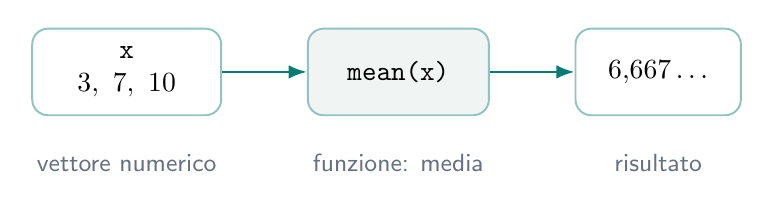
\begin{tikzpicture}[x=1cm,y=1cm]
\node[pFlow,minimum width=2.4cm] (x) at(1.3,1.45){\texttt{x}\\$3,\ 7,\ 10$};
\node[pFlow,minimum width=2.3cm,fill=GeoTint] (f) at(4.75,1.45){\texttt{mean(x)}};
\node[pFlow,minimum width=2.1cm] (r) at(8.05,1.45){$6{,}667\ldots$};
\draw[pEdge](x)--(f);\draw[pEdge](f)--(r);
\node[pNote] at(1.3,.3){vettore numerico};
\node[pNote] at(4.75,.3){funzione: media};
\node[pNote] at(8.05,.3){risultato};
\end{tikzpicture}
\PInfo{La console esegue un’istruzione. Il file \texttt{.R} permette di correggerla, salvarla e ripetere l’intera sequenza.}

\end{minipage}% 
\end{lrbox}
\begin{lrbox}{\PilotRightBox}%
\begin{minipage}[t]{7.55cm}\raggedright\color{Ink}\fontsize{11.3}{14.8}\selectfont

\PCode{R · assegnare e calcolare}{03_oggetti.R}
\PBody{\texttt{<-} assegna un valore a un nome. Le parentesi contengono gli argomenti della funzione.}
\PSmall{Dopo \texttt{\#} si scrive un commento: R lo ignora durante l’esecuzione. Maiuscole e minuscole distinguono nomi diversi.}

\end{minipage}% 
\end{lrbox}

\begin{frame}[plain]\hypertarget{slide3}{}
\bookmark[level=1,page=3]{R: oggetti, istruzioni e risultati}
\begin{tikzpicture}[remember picture,overlay]
\PilotChrome{R: oggetti, istruzioni e risultati}{PRIMI PASSI IN R}{3}{Un oggetto conserva un valore; una funzione produce un risultato. Lo script documenta le operazioni eseguite.}
\node[anchor=north west,inner sep=0] at ([xshift=0.96cm,yshift=-2.13cm]current page.north west) {\usebox{\PilotLeftBox}};
\node[anchor=north west,inner sep=0] at ([xshift=11.52cm,yshift=-2.13cm]current page.north west) {\usebox{\PilotRightBox}};
\end{tikzpicture}
\end{frame}

% SLIDE 004 | Dove, quando e che cosa si misura | REVISIONE COMPLETA
\begin{lrbox}{\PilotLeftBox}%
\begin{minipage}[t]{10.05cm}\raggedright\color{Ink}\fontsize{11.3}{14.8}\selectfont

\PLabel{La posizione fa parte del dato}
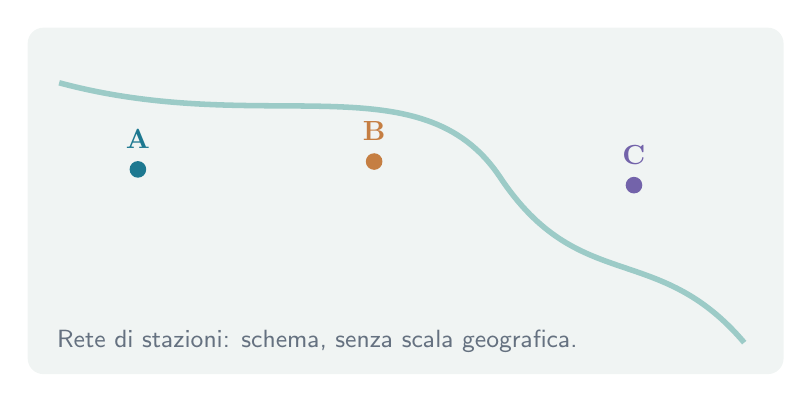
\begin{tikzpicture}[x=1cm,y=1cm]
\fill[GeoTint,rounded corners=2mm] (0,0) rectangle (9.6,4.4);
\draw[Classical!40,line width=2pt] (.4,3.7)..controls(3,3)and(5,4)..(6,2.5)..controls(7,1)and(8,1.7)..(9.1,.4);
\foreach \xx/\yy/\st/\col in {1.4/2.6/A/GeoA,4.4/2.7/B/GeoB,7.7/2.4/C/GeoC}{
 \fill[\col] (\xx,\yy) circle(3pt);
 \node[above=4pt,font=\bfseries,text=\col] at(\xx,\yy){\st};}
\node[pNote,anchor=south west] at(.25,.15){Rete di stazioni: schema, senza scala geografica.};
\end{tikzpicture}
\PBody{La stessa grandezza può variare nello spazio e nel tempo. Coordinate, data, profondità e strumento permettono di interpretare ciascuna misura.}

\end{minipage}%
\end{lrbox}
\typeout{FULLBOX:004:L:\the\ht\PilotLeftBox:\the\dp\PilotLeftBox}
\begin{lrbox}{\PilotRightBox}%
\begin{minipage}[t]{7.55cm}\raggedright\color{Ink}\fontsize{11.3}{14.8}\selectfont

\PLabel{Tre domande prima del calcolo}
\PBody{\textbf{Dove?} Stazione A, campione superficiale.\\[2mm]
\textbf{Quando?} Data e intervallo di acquisizione.\\[2mm]
\textbf{Che cosa?} Concentrazione, in mg/L.}
\vspace{3mm}
\PCode{R · il nome ricorda l'unità}{04_unita.R}
\PSmall{Le operazioni agiscono su tutti gli elementi del vettore. R non controlla automaticamente la coerenza delle unità.}

\end{minipage}%
\end{lrbox}
\typeout{FULLBOX:004:R:\the\ht\PilotRightBox:\the\dp\PilotRightBox}
\begin{frame}[plain]\hypertarget{slide4}{}
\bookmark[level=1,page=4]{Dove, quando e che cosa si misura}
\begin{tikzpicture}[remember picture,overlay]
\PilotChrome{Dove, quando e che cosa si misura}{DATI NELLE SCIENZE DELLA TERRA}{4}{Il valore numerico va associato a unità, luogo, tempo e procedura di misura.}
\node[anchor=north west,inner sep=0] at ([xshift=0.96cm,yshift=-2.13cm]current page.north west) {\usebox{\PilotLeftBox}};
\node[anchor=north west,inner sep=0] at ([xshift=11.52cm,yshift=-2.13cm]current page.north west) {\usebox{\PilotRightBox}};
\end{tikzpicture}
\end{frame}

% SLIDE 005 | R, fogli di calcolo e sistemi GIS | REVISIONE COMPLETA
\begin{lrbox}{\PilotLeftBox}%
\begin{minipage}[t]{10.05cm}\raggedright\color{Ink}\fontsize{11.3}{14.8}\selectfont

\PLabel{Scegliere lo strumento per l'operazione}
\renewcommand{\arraystretch}{1.65}
\begin{tabular}{@{}p{2.5cm}p{6.8cm}@{}}\toprule
\textbf{Strumento}&\textbf{Operazioni tipiche}\\\midrule
Foglio di calcolo&Inserimento e controllo visivo di una piccola tabella.\\
R&Trasformazioni documentate, stime, modelli e grafici ripetibili.\\
GIS&Geometrie, sistemi di riferimento, relazioni spaziali e cartografia.\\\bottomrule
\end{tabular}
\vspace{3mm}\PBody{Il progetto può utilizzare più programmi. Gli scambi richiedono nomi, unità e identificativi coerenti.}

\end{minipage}%
\end{lrbox}
\typeout{FULLBOX:005:L:\the\ht\PilotLeftBox:\the\dp\PilotLeftBox}
\begin{lrbox}{\PilotRightBox}%
\begin{minipage}[t]{7.55cm}\raggedright\color{Ink}\fontsize{11.3}{14.8}\selectfont

\PLabel{Passaggi da documentare}
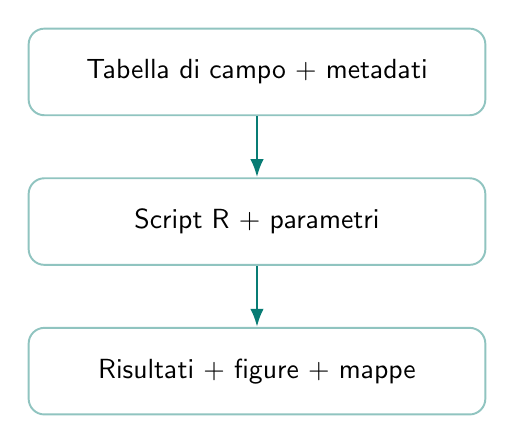
\begin{tikzpicture}[x=1cm,y=1cm]
\node[pFlow,minimum width=5.8cm] (a) at(3.5,5.7){Tabella di campo + metadati};
\node[pFlow,minimum width=5.8cm] (b) at(3.5,3.8){Script R + parametri};
\node[pFlow,minimum width=5.8cm] (c) at(3.5,1.9){Risultati + figure + mappe};
\draw[pEdge](a)--(b);\draw[pEdge](b)--(c);
\end{tikzpicture}
\PInfo{Un CSV conserva una tabella. Informazioni su sensori, unità e coordinate devono essere documentate a parte.}

\end{minipage}%
\end{lrbox}
\typeout{FULLBOX:005:R:\the\ht\PilotRightBox:\the\dp\PilotRightBox}
\begin{frame}[plain]\hypertarget{slide5}{}
\bookmark[level=1,page=5]{R, fogli di calcolo e sistemi GIS}
\begin{tikzpicture}[remember picture,overlay]
\PilotChrome{R, fogli di calcolo e sistemi GIS}{STRUMENTI DI LAVORO}{5}{Conservare dati, parametri e script consente di ricostruire il risultato anche quando si usano programmi diversi.}
\node[anchor=north west,inner sep=0] at ([xshift=0.96cm,yshift=-2.13cm]current page.north west) {\usebox{\PilotLeftBox}};
\node[anchor=north west,inner sep=0] at ([xshift=11.52cm,yshift=-2.13cm]current page.north west) {\usebox{\PilotRightBox}};
\end{tikzpicture}
\end{frame}

% SLIDE 006 | Dalla misura alla tabella in R | REVISIONE COMPLETA
\begin{lrbox}{\PilotLeftBox}%
\begin{minipage}[t]{10.05cm}\raggedright\color{Ink}\fontsize{11.3}{14.8}\selectfont
\PLabel{Schema della tabella}
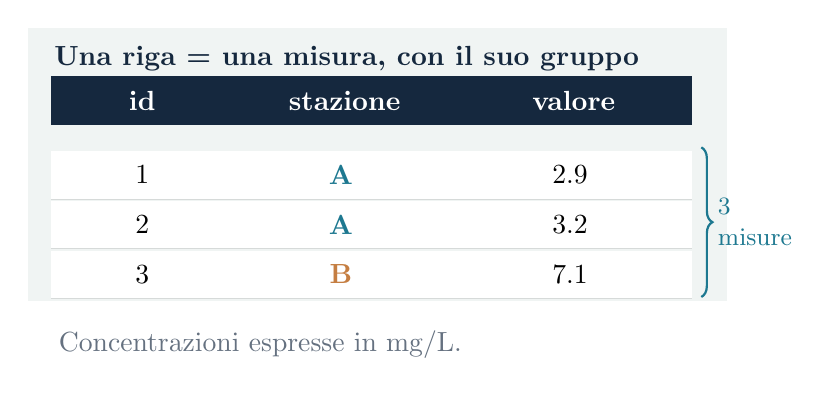
\begin{tikzpicture}[x=.97cm,y=1cm]
 \fill[GeoTint] (.1,1.05) rectangle (9.25,4.52);
 \node[anchor=west,font=\bfseries\fontsize{10.4}{12.5}\selectfont,color=Navy] at (.32,4.13) {Una riga = una misura, con il suo gruppo};
 \foreach \x/\w/\name in {.4/2.4/id,2.8/2.9/stazione,5.7/3.1/valore} {
   \fill[Navy] (\x,3.28) rectangle ++(\w,.62);
   \node[anchor=center,color=white,font=\bfseries\fontsize{9.8}{12}\selectfont] at (\x+\w/2,3.59) {\name};}
 \foreach \y/\id/\st/\v/\col in {2.65/1/A/2.9/GeoA,2.02/2/A/3.2/GeoA,1.39/3/B/7.1/GeoB} {
   \fill[white] (.4,\y-.31) rectangle (8.8,\y+.30);
   \draw[Rule] (.4,\y-.31)--(8.8,\y-.31);
   \node at (1.6,\y) {\id};
   \node[text=\col, font=\bfseries] at (4.2,\y) {\st};
   \node at (7.2,\y) {\v};}
 \draw[GeoA,thick,decorate,decoration={brace,amplitude=4pt}] (8.92,3.0)--(8.92,1.1)
   node[midway,xshift=.08cm,right,font=\fontsize{8.8}{11}\selectfont,align=left] {3\\misure};
 \node[anchor=west,font=\fontsize{10.3}{13.1}\selectfont,color=Muted] at (.38,.50) {Concentrazioni espresse in mg/L.};
\end{tikzpicture}
\vspace{2mm}
\PInfo{\textbf{Vettore}: una colonna omogenea. \textbf{Data frame}: colonne associate alle medesime righe. L'identificativo distingue le osservazioni.}

\end{minipage}%
\end{lrbox}
\typeout{FULLBOX:006:L:\the\ht\PilotLeftBox:\the\dp\PilotLeftBox}
\begin{lrbox}{\PilotRightBox}%
\begin{minipage}[t]{7.55cm}\raggedright\color{Ink}\fontsize{11.3}{14.8}\selectfont

\PLabel{Esempio minimo e leggibile}
\PCode{R · costruire una piccola tabella}{06_tabella.R}
\PSmall{\texttt{data.frame()} accoppia le colonne per posizione. \texttt{factor()} dichiara una variabile categoriale; \texttt{str()} mostra la struttura dell'oggetto.}

\end{minipage}%
\end{lrbox}
\typeout{FULLBOX:006:R:\the\ht\PilotRightBox:\the\dp\PilotRightBox}
\begin{frame}[plain]\hypertarget{slide6}{}
\bookmark[level=1,page=6]{Dalla misura alla tabella in R}
\begin{tikzpicture}[remember picture,overlay]
\PilotChrome{Dalla misura alla tabella in R}{STRUTTURE DATI}{6}{Il calcolo per riga ha senso soltanto se tutte le colonne si riferiscono alla stessa osservazione.}
\node[anchor=north west,inner sep=0] at ([xshift=0.96cm,yshift=-2.13cm]current page.north west) {\usebox{\PilotLeftBox}};
\node[anchor=north west,inner sep=0] at ([xshift=11.52cm,yshift=-2.13cm]current page.north west) {\usebox{\PilotRightBox}};
\end{tikzpicture}
\end{frame}

% SLIDE 007 | Organizzare un progetto riproducibile | REVISIONE COMPLETA
\begin{lrbox}{\PilotLeftBox}%
\begin{minipage}[t]{10.05cm}\raggedright\color{Ink}\fontsize{11.3}{14.8}\selectfont

\PLabel{Il pacchetto della lezione}
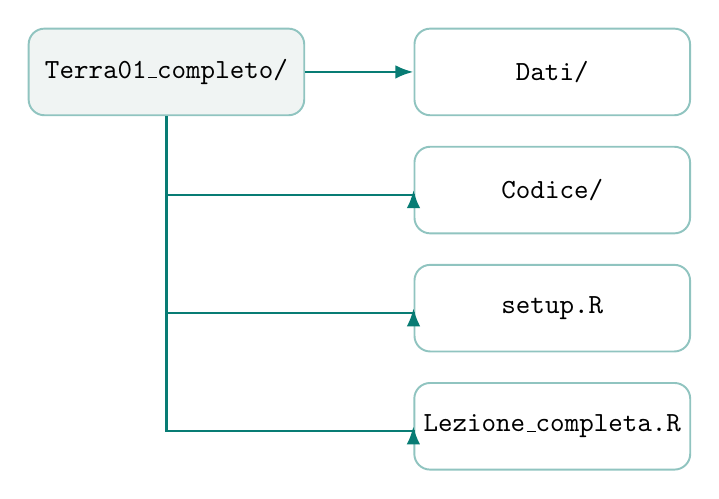
\begin{tikzpicture}[x=1cm,y=1cm]
\node[pFlow,minimum width=3.5cm,fill=GeoTint] (p) at(2.1,5.6){\texttt{Terra01\_completo/}};
\node[pFlow,minimum width=3.5cm] (a) at(7,5.6){\texttt{Dati/}};
\node[pFlow,minimum width=3.5cm] (b) at(7,4.1){\texttt{Codice/}};
\node[pFlow,minimum width=3.5cm] (c) at(7,2.6){\texttt{setup.R}};
\node[pFlow,minimum width=3.5cm] (d) at(7,1.1){\texttt{Lezione\_completa.R}};
\draw[pEdge](p)--(a);\draw[pEdge](p.south)--++(0,-1)-|(b.west);
\draw[pEdge](p.south)--++(0,-2.5)-|(c.west);
\draw[pEdge](p.south)--++(0,-4)-|(d.west);
\end{tikzpicture}
\PSmall{\texttt{Dati/} contiene CSV conservati; \texttt{Codice/} raccoglie i frammenti numerati per slide. Lo script completo segue l'ordine della lezione.}

\end{minipage}%
\end{lrbox}
\typeout{FULLBOX:007:L:\the\ht\PilotLeftBox:\the\dp\PilotLeftBox}
\begin{lrbox}{\PilotRightBox}%
\begin{minipage}[t]{7.55cm}\raggedright\color{Ink}\fontsize{11.3}{14.8}\selectfont

\PCode{R · iniziare dalla cartella del progetto}{07_avvio.R}
\PBody{Aprire \texttt{Terra01.Rproj} in RStudio, oppure impostare la cartella estratta come directory di lavoro.}
\vspace{2mm}\PSmall{\texttt{setup.R} prepara \texttt{terra}, l'anteprima di Terra01, e \texttt{demo}, la serie meteorologica simulata. \texttt{sessionInfo()} registra R e i pacchetti utilizzati.}

\end{minipage}%
\end{lrbox}
\typeout{FULLBOX:007:R:\the\ht\PilotRightBox:\the\dp\PilotRightBox}
\begin{frame}[plain]\hypertarget{slide7}{}
\bookmark[level=1,page=7]{Organizzare un progetto riproducibile}
\begin{tikzpicture}[remember picture,overlay]
\PilotChrome{Organizzare un progetto riproducibile}{DATI E SCRIPT}{7}{Eseguire lo script dalla cartella del progetto rende validi i percorsi relativi usati negli esempi.}
\node[anchor=north west,inner sep=0] at ([xshift=0.96cm,yshift=-2.13cm]current page.north west) {\usebox{\PilotLeftBox}};
\node[anchor=north west,inner sep=0] at ([xshift=11.52cm,yshift=-2.13cm]current page.north west) {\usebox{\PilotRightBox}};
\end{tikzpicture}
\end{frame}

% SLIDE 008 | Dalla domanda alla rappresentazione | REVISIONE COMPLETA
\begin{lrbox}{\PilotLeftBox}%
\begin{minipage}[t]{10.05cm}\raggedright\color{Ink}\fontsize{11.3}{14.8}\selectfont

\PLabel{La tabella contiene misure; la domanda sceglie il riepilogo}
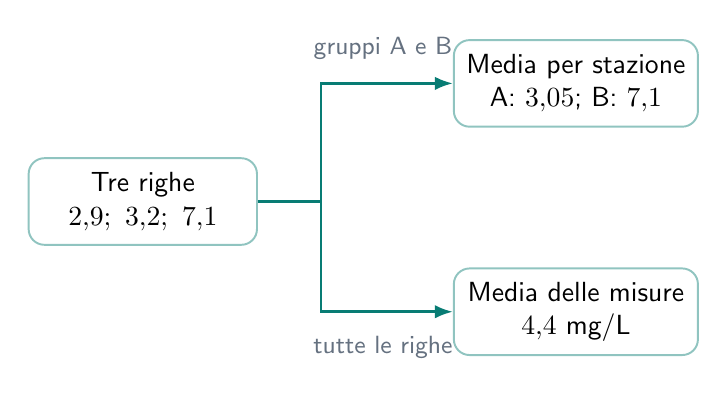
\begin{tikzpicture}[x=1cm,y=1cm]
\node[pFlow,minimum width=2.9cm] (t) at(1.65,2.8){Tre righe\\$2{,}9;\ 3{,}2;\ 7{,}1$};
\node[pFlow,minimum width=3.1cm] (g) at(7.15,4.3){Media per stazione\\A: $3{,}05$; B: $7{,}1$};
\node[pFlow,minimum width=3.1cm] (m) at(7.15,1.4){Media delle misure\\$4{,}4$ mg/L};
\draw[pEdge](t.east)--++(.8,0)|-(g.west);
\draw[pEdge](t.east)--++(.8,0)|-(m.west);
\node[pNote] at(4.7,4.75){gruppi A e B};
\node[pNote] at(4.7,.95){tutte le righe};
\end{tikzpicture}
\PBody{La scelta del grafico segue la quantità calcolata: confronto fra stazioni, distribuzione delle misure oppure variazione nel tempo.}

\end{minipage}%
\end{lrbox}
\typeout{FULLBOX:008:L:\the\ht\PilotLeftBox:\the\dp\PilotLeftBox}
\begin{lrbox}{\PilotRightBox}%
\begin{minipage}[t]{7.55cm}\raggedright\color{Ink}\fontsize{11.3}{14.8}\selectfont

\PCode{R · una colonna, due riepiloghi}{08_riepiloghi.R}
\PSmall{\texttt{\$} seleziona una colonna. In \texttt{tapply(x, gruppo, mean)}, il secondo argomento definisce i gruppi.}
\vspace{2mm}\PInfo{Questi tre valori sono un esempio didattico. L'oggetto \texttt{terra} contiene invece le 40 misure del laboratorio.}

\end{minipage}%
\end{lrbox}
\typeout{FULLBOX:008:R:\the\ht\PilotRightBox:\the\dp\PilotRightBox}
\begin{frame}[plain]\hypertarget{slide8}{}
\bookmark[level=1,page=8]{Dalla domanda alla rappresentazione}
\begin{tikzpicture}[remember picture,overlay]
\PilotChrome{Dalla domanda alla rappresentazione}{UNITÀ E AGGREGAZIONE}{8}{Aggregare cambia l’unità descritta dal risultato. Va indicato se si stanno confrontando misure, stazioni o periodi.}
\node[anchor=north west,inner sep=0] at ([xshift=0.96cm,yshift=-2.13cm]current page.north west) {\usebox{\PilotLeftBox}};
\node[anchor=north west,inner sep=0] at ([xshift=11.52cm,yshift=-2.13cm]current page.north west) {\usebox{\PilotRightBox}};
\end{tikzpicture}
\end{frame}

% SLIDE 009 | Metadati e versioni dei dati | REVISIONE COMPLETA
\begin{lrbox}{\PilotLeftBox}%
\begin{minipage}[t]{10.05cm}\raggedright\color{Ink}\fontsize{11.3}{14.8}\selectfont

\PLabel{La misura e la sua scheda}
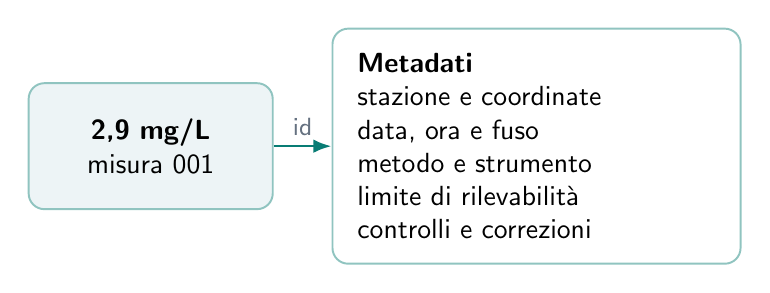
\begin{tikzpicture}[x=1cm,y=1cm]
\node[pFlow,minimum width=3.1cm,minimum height=1.6cm,fill=GeoA!8] (v) at(1.8,3.1){\textbf{2,9 mg/L}\\misura 001};
\node[pFlow,text width=4.55cm,align=left,inner sep=9pt] (m) at(6.7,3.1){\textbf{Metadati}\\stazione e coordinate\\data, ora e fuso\\metodo e strumento\\limite di rilevabilità\\controlli e correzioni};
\draw[pEdge](v)--node[above,pNote]{id}(m);
\end{tikzpicture}
\PBody{I dati originali restano conservati. Una correzione produce una nuova versione, accompagnata da motivo, data e procedura.}

\end{minipage}%
\end{lrbox}
\typeout{FULLBOX:009:L:\the\ht\PilotLeftBox:\the\dp\PilotLeftBox}
\begin{lrbox}{\PilotRightBox}%
\begin{minipage}[t]{7.55cm}\raggedright\color{Ink}\fontsize{11.3}{14.8}\selectfont

\PLabel{Un dizionario delle colonne}
\renewcommand{\arraystretch}{1.4}
\begin{tabular}{@{}ll@{}}\toprule
\textbf{Nome}&\textbf{Significato}\\\midrule
\texttt{stazione}&Etichetta A, B o C\\
\texttt{valore}&Concentrazione in mg/L\\\bottomrule
\end{tabular}
\vspace{3mm}\PCode{R · leggere nomi e dimensioni}{09_schema.R}
\PSmall{Dimensioni e nomi sono controlli iniziali. Le condizioni di misura sono descritte nei metadati.}

\end{minipage}%
\end{lrbox}
\typeout{FULLBOX:009:R:\the\ht\PilotRightBox:\the\dp\PilotRightBox}
\begin{frame}[plain]\hypertarget{slide9}{}
\bookmark[level=1,page=9]{Metadati e versioni dei dati}
\begin{tikzpicture}[remember picture,overlay]
\PilotChrome{Metadati e versioni dei dati}{DOCUMENTARE IL CONTESTO}{9}{Il dizionario dei dati spiega che cosa rappresentano le colonne; il registro delle modifiche documenta come sono cambiate.}
\node[anchor=north west,inner sep=0] at ([xshift=0.96cm,yshift=-2.13cm]current page.north west) {\usebox{\PilotLeftBox}};
\node[anchor=north west,inner sep=0] at ([xshift=11.52cm,yshift=-2.13cm]current page.north west) {\usebox{\PilotRightBox}};
\end{tikzpicture}
\end{frame}

% SLIDE 010 | Dalla domanda scientifica alla conclusione | REVISIONE COMPLETA
\begin{lrbox}{\PilotLeftBox}%
\begin{minipage}[t]{10.05cm}\raggedright\color{Ink}\fontsize{11.3}{14.8}\selectfont
\PLabel{Catena delle operazioni}
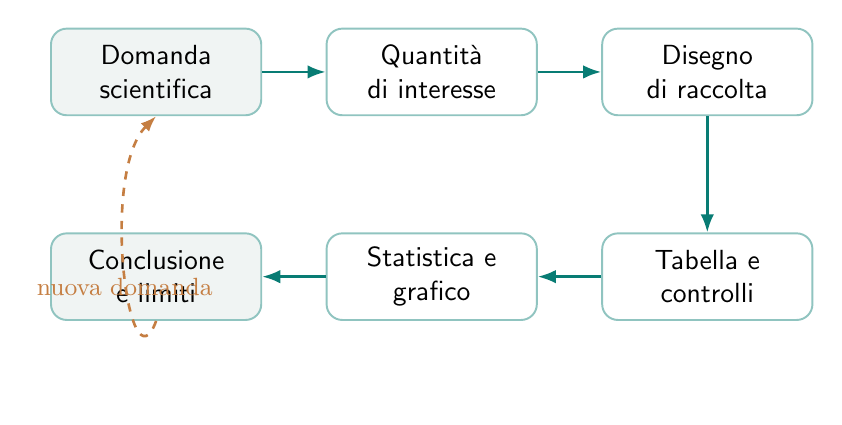
\begin{tikzpicture}[x=1cm,y=1cm]
 \node[pFlow,minimum width=2.67cm,fill=GeoTint] (a) at (1.5,4.95) {Domanda\\scientifica};
 \node[pFlow,minimum width=2.67cm] (b) at (5.0,4.95) {Quantità\\di interesse};
 \node[pFlow,minimum width=2.67cm] (c) at (8.5,4.95) {Disegno\\di raccolta};
 \node[pFlow,minimum width=2.67cm] (d) at (8.5,2.35) {Tabella e\\controlli};
 \node[pFlow,minimum width=2.67cm] (e) at (5.0,2.35) {Statistica e\\grafico};
 \node[pFlow,minimum width=2.67cm,fill=GeoTint] (f) at (1.5,2.35) {Conclusione\\e limiti};
 \draw[pEdge] (a)--(b);\draw[pEdge] (b)--(c);\draw[pEdge] (c)--(d);
 \draw[pEdge] (d)--(e);\draw[pEdge] (e)--(f);
 \draw[GeoB,dashed,line width=.95pt,-{Latex[length=2mm]}] (f.south) to[out=-110,in=-135] node[below,font=\fontsize{9}{11}\selectfont,color=GeoB] {nuova domanda} (a.south);
\end{tikzpicture}
\PInfo{La scelta della quantità da stimare precede il programma: un risultato numerico non determina da solo quale domanda sia stata affrontata.}

\end{minipage}%
\end{lrbox}
\typeout{FULLBOX:010:L:\the\ht\PilotLeftBox:\the\dp\PilotLeftBox}
\begin{lrbox}{\PilotRightBox}%
\begin{minipage}[t]{7.55cm}\raggedright\color{Ink}\fontsize{11.3}{14.8}\selectfont
\PLabel{Dal dato alla stima}
\PBody{Una tabella con \(N\) righe conserva coppie osservate \((g_i,x_i)\). Una procedura \(f\), insieme alle scelte di analisi \(\mathcal A\), produce una statistica:}
\vspace{1mm}
\[D=\{(g_i,x_i)\}_{i=1}^{N},\qquad \widehat\theta=f(D;\mathcal A).\]
\PSmall{\(g_i\) è il gruppo; \(x_i\) è la misura. \(\widehat\theta\) è il valore ricavato dal campione, mentre \(\theta\) indica la quantità definita dalla domanda.}
\vspace{2mm}
\PInfo{Registro minimo: dati utilizzati, selezioni, parametri, unità di misura e programma che produce il risultato.}

\end{minipage}%
\end{lrbox}
\typeout{FULLBOX:010:R:\the\ht\PilotRightBox:\the\dp\PilotRightBox}
\begin{frame}[plain]\hypertarget{slide10}{}
\bookmark[level=1,page=10]{Dalla domanda scientifica alla conclusione}
\begin{tikzpicture}[remember picture,overlay]
\PilotChrome{Dalla domanda scientifica alla conclusione}{METODO DI ANALISI}{10}{Una conclusione è ricostruibile quando è possibile risalire dal risultato alle osservazioni e alle scelte adottate.}
\node[anchor=north west,inner sep=0] at ([xshift=0.96cm,yshift=-2.13cm]current page.north west) {\usebox{\PilotLeftBox}};
\node[anchor=north west,inner sep=0] at ([xshift=11.52cm,yshift=-2.13cm]current page.north west) {\usebox{\PilotRightBox}};
\end{tikzpicture}
\end{frame}

% SLIDE 011 | Domande ambientali e quantità da stimare | REVISIONE COMPLETA
\begin{lrbox}{\PilotLeftBox}%
\begin{minipage}[t]{10.05cm}\raggedright\color{Ink}\fontsize{11.3}{14.8}\selectfont

\PLabel{Domande simili possono richiedere dati diversi}
\renewcommand{\arraystretch}{1.55}
\begin{tabular}{@{}p{4.65cm}p{4.65cm}@{}}\toprule
\textbf{Domanda}&\textbf{Informazioni necessarie}\\\midrule
Qual è la temperatura media del mese?&Serie nel mese, orari e copertura temporale.\\
Quale stazione è più calda?&Periodi comparabili, quota e condizioni di esposizione.\\
La temperatura cresce nel tempo?&Serie sufficientemente lunga, stagionalità e storia strumentale.\\\bottomrule
\end{tabular}

\end{minipage}%
\end{lrbox}
\typeout{FULLBOX:011:L:\the\ht\PilotLeftBox:\the\dp\PilotLeftBox}
\begin{lrbox}{\PilotRightBox}%
\begin{minipage}[t]{7.55cm}\raggedright\color{Ink}\fontsize{11.3}{14.8}\selectfont

\PLabel{Un esempio di formalizzazione}
\PBody{Per confrontare due stazioni nello stesso periodo:}
\[\Delta=\mu_A-\mu_B.\]
\PSmall{\(\mu_A\) e \(\mu_B\): temperature medie del periodo e delle stazioni dichiarate. \(\Delta\) si esprime in °C.}
\vspace{3mm}\PBody{La differenza campionaria è}
\[\widehat\Delta=\bar x_A-\bar x_B.\]
\PInfo{L'interpretazione richiede misure confrontabili e un disegno adatto alla popolazione che interessa.}

\end{minipage}%
\end{lrbox}
\typeout{FULLBOX:011:R:\the\ht\PilotRightBox:\the\dp\PilotRightBox}
\begin{frame}[plain]\hypertarget{slide11}{}
\bookmark[level=1,page=11]{Domande ambientali e quantità da stimare}
\begin{tikzpicture}[remember picture,overlay]
\PilotChrome{Domande ambientali e quantità da stimare}{DOMANDA E DISEGNO}{11}{La domanda precisa grandezza, popolazione, spazio e periodo. Queste scelte precedono la formula.}
\node[anchor=north west,inner sep=0] at ([xshift=0.96cm,yshift=-2.13cm]current page.north west) {\usebox{\PilotLeftBox}};
\node[anchor=north west,inner sep=0] at ([xshift=11.52cm,yshift=-2.13cm]current page.north west) {\usebox{\PilotRightBox}};
\end{tikzpicture}
\end{frame}

% SLIDE 012 | Statistica: osservazioni e incertezza | REVISIONE COMPLETA
\begin{lrbox}{\PilotLeftBox}%
\begin{minipage}[t]{10.05cm}\raggedright\color{Ink}\fontsize{11.3}{14.8}\selectfont

\PLabel{Ripetere il campionamento cambia la stima}
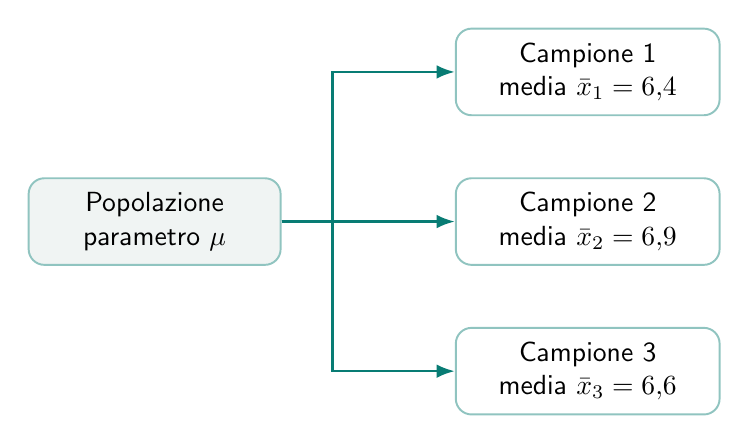
\begin{tikzpicture}[x=1cm,y=1cm]
\node[pFlow,minimum width=3.2cm,fill=GeoTint] (p) at(1.9,3.2){Popolazione\\parametro $\mu$};
\foreach \yy/\name/\mean in {5.1/1/{6{,}4},3.2/2/{6{,}9},1.3/3/{6{,}6}}{
 \node[pFlow,minimum width=3.35cm] (s\name) at(7.4,\yy){Campione \name\\media $\bar x_{\name}=\mean$};
 \draw[pEdge](p.east)--++(.65,0)|-(s\name.west);
}
\end{tikzpicture}
\PSmall{Valori illustrativi. Anche applicando la stessa procedura, campioni diversi possono dare medie diverse.}

\end{minipage}%
\end{lrbox}
\typeout{FULLBOX:012:L:\the\ht\PilotLeftBox:\the\dp\PilotLeftBox}
\begin{lrbox}{\PilotRightBox}%
\begin{minipage}[t]{7.55cm}\raggedright\color{Ink}\fontsize{11.3}{14.8}\selectfont

\PLabel{Parametro e statistica}
\PBody{\(\mu\) descrive la popolazione o il modello. \(\bar x\) è calcolata sulle osservazioni disponibili.}
\[\bar x=\frac{1}{n}\sum_{i=1}^{n}x_i.\]
\PBody{L'incertezza riguarda quanto cambierebbe la stima ripetendo la procedura di raccolta.}
\vspace{2mm}\PInfo{Aumentare il numero di misure riduce alcune componenti casuali. La selezione dei siti e gli errori sistematici richiedono controlli specifici.}

\end{minipage}%
\end{lrbox}
\typeout{FULLBOX:012:R:\the\ht\PilotRightBox:\the\dp\PilotRightBox}
\begin{frame}[plain]\hypertarget{slide12}{}
\bookmark[level=1,page=12]{Statistica: osservazioni e incertezza}
\begin{tikzpicture}[remember picture,overlay]
\PilotChrome{Statistica: osservazioni e incertezza}{POPOLAZIONE E CAMPIONE}{12}{Una stima è accompagnata da un ambito di validità e da una valutazione della sua incertezza.}
\node[anchor=north west,inner sep=0] at ([xshift=0.96cm,yshift=-2.13cm]current page.north west) {\usebox{\PilotLeftBox}};
\node[anchor=north west,inner sep=0] at ([xshift=11.52cm,yshift=-2.13cm]current page.north west) {\usebox{\PilotRightBox}};
\end{tikzpicture}
\end{frame}

% SLIDE 013 | Tipi di variabili | REVISIONE COMPLETA
\begin{lrbox}{\PilotLeftBox}%
\begin{minipage}[t]{10.05cm}\raggedright\color{Ink}\fontsize{11.3}{14.8}\selectfont

\PLabel{Il tipo determina i calcoli sensati}
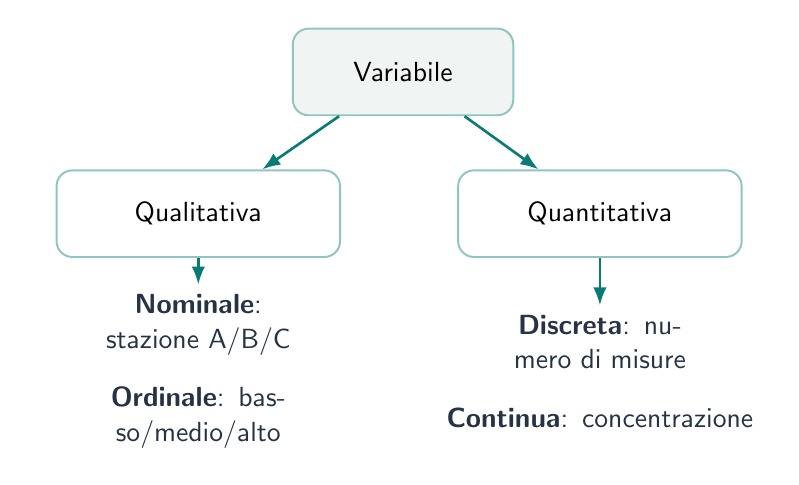
\begin{tikzpicture}[x=1cm,y=1cm]
\node[pFlow,minimum width=2.8cm,fill=GeoTint] (v) at(4.8,5.9){Variabile};
\node[pFlow,minimum width=3.6cm] (q) at(2.2,4.1){Qualitativa};
\node[pFlow,minimum width=3.6cm] (n) at(7.3,4.1){Quantitativa};
\draw[pEdge](v)--(q);\draw[pEdge](v)--(n);
\node[pLabel,text width=4.1cm] (q2) at(2.2,2.1){\textbf{Nominale}: stazione A/B/C\\[3mm]\textbf{Ordinale}: basso/medio/alto};
\node[pLabel,text width=4.1cm] (n2) at(7.3,2.1){\textbf{Discreta}: numero di misure\\[3mm]\textbf{Continua}: concentrazione};
\draw[pEdge](q)--(q2);\draw[pEdge](n)--(n2);
\end{tikzpicture}
\PSmall{Un codice numerico assegnato a una categoria conserva il significato di etichetta. La sua media può essere priva di interpretazione.}

\end{minipage}%
\end{lrbox}
\typeout{FULLBOX:013:L:\the\ht\PilotLeftBox:\the\dp\PilotLeftBox}
\begin{lrbox}{\PilotRightBox}%
\begin{minipage}[t]{7.55cm}\raggedright\color{Ink}\fontsize{11.3}{14.8}\selectfont

\PCode{R · categorie e numeri}{13_tipi.R}
\PSmall{\texttt{factor()} memorizza categorie. I livelli sono i valori ammessi; \texttt{table()} conta quante osservazioni appartengono a ogni livello.}
\vspace{2mm}\PInfo{In Terra01, \texttt{stazione} identifica un gruppo e \texttt{valore} contiene una concentrazione in mg/L.}

\end{minipage}%
\end{lrbox}
\typeout{FULLBOX:013:R:\the\ht\PilotRightBox:\the\dp\PilotRightBox}
\begin{frame}[plain]\hypertarget{slide13}{}
\bookmark[level=1,page=13]{Tipi di variabili}
\begin{tikzpicture}[remember picture,overlay]
\PilotChrome{Tipi di variabili}{LEGGERE LA TABELLA}{13}{Il significato della variabile guida riassunti e grafici; la sola forma con cui è salvata nel file può essere ingannevole.}
\node[anchor=north west,inner sep=0] at ([xshift=0.96cm,yshift=-2.13cm]current page.north west) {\usebox{\PilotLeftBox}};
\node[anchor=north west,inner sep=0] at ([xshift=11.52cm,yshift=-2.13cm]current page.north west) {\usebox{\PilotRightBox}};
\end{tikzpicture}
\end{frame}

% SLIDE 014 | Popolazione, stazioni e misure replicate | REVISIONE COMPLETA
\begin{lrbox}{\PilotLeftBox}%
\begin{minipage}[t]{10.05cm}\raggedright\color{Ink}\fontsize{11.3}{14.8}\selectfont
\PLabel{Ambito, stazioni e misure}
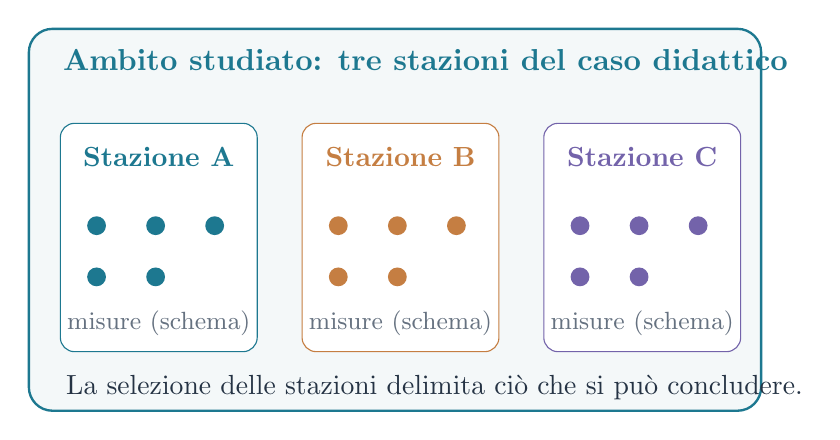
\begin{tikzpicture}[x=1cm,y=1cm]
 \draw[GeoA,fill=GeoA!5,line width=.85pt,rounded corners=3mm] (.25,.6) rectangle (9.55,5.45);
 \node[anchor=west,color=GeoA,font=\bfseries\fontsize{10.7}{13}\selectfont] at (.56,5.05) {Ambito studiato: tre stazioni del caso didattico};
 \foreach \x/\lab/\col/\num in {.65/A/GeoA/5,3.72/B/GeoB/4,6.79/C/GeoC/4}{
  \draw[\col,fill=white,rounded corners=1.8mm] (\x,1.35) rectangle ++(2.50,2.9);
  \node[font=\bfseries,color=\col] at (\x+1.25,3.82) {Stazione \lab};
  \foreach \dx/\dy in {0/0,.75/0,1.5/0,0/-.65,.75/-.65}{\node[circle,fill=\col,inner sep=2.4pt] at (\x+.46+\dx,2.95+\dy) {};}
  \node[font=\fontsize{9.2}{11}\selectfont,color=Muted] at (\x+1.25,1.71) {misure (schema)};
 }
 \node[anchor=west,font=\fontsize{9.8}{12.6}\selectfont,color=Ink] at (.6,.90) {La selezione delle stazioni delimita ciò che si può concludere.};
\end{tikzpicture}
\vspace{1mm}
\PInfo{\textbf{Unità}: stazione o misura. Nei dati reali, ripetere una lettura non crea automaticamente un'altra unità indipendente.}

\end{minipage}%
\end{lrbox}
\typeout{FULLBOX:014:L:\the\ht\PilotLeftBox:\the\dp\PilotLeftBox}
\begin{lrbox}{\PilotRightBox}%
\begin{minipage}[t]{7.55cm}\raggedright\color{Ink}\fontsize{11.3}{14.8}\selectfont

\PLabel{Notazione e ambito della conclusione}
\[G=3,\qquad N=\sum_{g=1}^{G}n_g.\]
\PBody{\(G\): numero di stazioni; \(n_g\): misure nella stazione \(g\); \(N\): numero totale di righe. Nello scenario iniziale \(n_A=20\), \(n_B=n_C=10\), quindi \(N=40\).}
\vspace{3mm}\PInfo{Il caso didattico considera le tre stazioni. Una media territoriale richiederebbe anche informazioni sulle aree o sui volumi rappresentati. Il generatore produce misure indipendenti entro e fra stazioni.}

\end{minipage}%
\end{lrbox}
\typeout{FULLBOX:014:R:\the\ht\PilotRightBox:\the\dp\PilotRightBox}
\begin{frame}[plain]\hypertarget{slide14}{}
\bookmark[level=1,page=14]{Popolazione, stazioni e misure replicate}
\begin{tikzpicture}[remember picture,overlay]
\PilotChrome{Popolazione, stazioni e misure replicate}{STATISTICA DI BASE}{14}{Quaranta righe non implicano quaranta stazioni; il livello dell’inferenza va dichiarato prima di calcolare la media.}
\node[anchor=north west,inner sep=0] at ([xshift=0.96cm,yshift=-2.13cm]current page.north west) {\usebox{\PilotLeftBox}};
\node[anchor=north west,inner sep=0] at ([xshift=11.52cm,yshift=-2.13cm]current page.north west) {\usebox{\PilotRightBox}};
\end{tikzpicture}
\end{frame}

% SLIDE 015 | Media, mediana e moda | REVISIONE COMPLETA
\begin{lrbox}{\PilotLeftBox}%
\begin{minipage}[t]{10.05cm}\raggedright\color{Ink}\fontsize{11.3}{14.8}\selectfont

\PLabel{Tre modi di riassumere la posizione}
\begin{tikzpicture}[x=.88cm,y=1cm]
\draw[pAxis](0,2.4)--(10.5,2.4);
\foreach \xx in {1,2,3,4,5,6,7,8,9,10}{\draw[Rule](\xx,2.32)--(\xx,2.48);\node[pNote,below] at(\xx,2.23){\xx};}
\foreach \xx/\yy in {2/2.8,3/2.8,3/3.25,4/2.8,9/2.8}{\fill[GeoA](\xx,\yy)circle(3pt);}
\draw[GeoB,thick,-{Latex}](4.2,4.35)--(4.2,3.55);
\node[pLabel,text=GeoB] at(5.9,4.4){Media $=4{,}2$};
\draw[Classical,thick,-{Latex}](3,.45)--(3,1.55);
\node[pLabel,text=Classical] at(3,.08){Mediana $=3$};
\end{tikzpicture}
\PBody{La media usa tutte le distanze numeriche. La mediana divide i dati ordinati in due metà. La moda identifica il valore o la categoria più frequente.}

\end{minipage}%
\end{lrbox}
\typeout{FULLBOX:015:L:\the\ht\PilotLeftBox:\the\dp\PilotLeftBox}
\begin{lrbox}{\PilotRightBox}%
\begin{minipage}[t]{7.55cm}\raggedright\color{Ink}\fontsize{11.3}{14.8}\selectfont

\PCode{R · tre riepiloghi}{15_posizione.R}
\PSmall{\texttt{sort()} ordina i valori. \texttt{table()} restituisce le frequenze: qui 3 compare due volte ed è l'unica moda.}
\vspace{2mm}\PInfo{In R, \texttt{mode()} descrive il modo di memorizzazione di un oggetto: non calcola la moda statistica.}

\end{minipage}%
\end{lrbox}
\typeout{FULLBOX:015:R:\the\ht\PilotRightBox:\the\dp\PilotRightBox}
\begin{frame}[plain]\hypertarget{slide15}{}
\bookmark[level=1,page=15]{Media, mediana e moda}
\begin{tikzpicture}[remember picture,overlay]
\PilotChrome{Media, mediana e moda}{INDICATORI DI POSIZIONE}{15}{La scelta dell’indicatore dipende dal tipo di variabile e dalla domanda; media e mediana possono differire molto.}
\node[anchor=north west,inner sep=0] at ([xshift=0.96cm,yshift=-2.13cm]current page.north west) {\usebox{\PilotLeftBox}};
\node[anchor=north west,inner sep=0] at ([xshift=11.52cm,yshift=-2.13cm]current page.north west) {\usebox{\PilotRightBox}};
\end{tikzpicture}
\end{frame}

% SLIDE 016 | Calcolare media e mediana | REVISIONE COMPLETA
\begin{lrbox}{\PilotLeftBox}%
\begin{minipage}[t]{10.05cm}\raggedright\color{Ink}\fontsize{11.3}{14.8}\selectfont

\PLabel{Dati ordinati: $x_{(1)}\le\cdots\le x_{(n)}$}
\[\bar x=\frac{x_1+\cdots+x_n}{n}.\]
\[\operatorname{med}(x)=\begin{cases}
x_{((n+1)/2)},& n\text{ dispari},\\[2mm]
\dfrac{x_{(n/2)}+x_{(n/2+1)}}{2},& n\text{ pari}.
\end{cases}\]
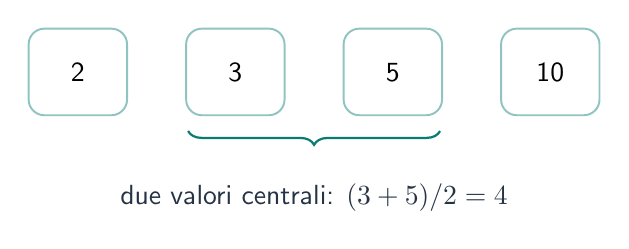
\begin{tikzpicture}[x=1cm,y=1cm]
\foreach \xx/\v in {1/2,3/3,5/5,7/10}{\node[pFlow,minimum width=1.25cm,fill=white] at(\xx,2.1){\v};}
\draw[Classical,thick,decorate,decoration={brace,mirror,amplitude=5pt}](2.4,1.35)--(5.6,1.35);
\node[pLabel] at(4,.5){due valori centrali: $(3+5)/2=4$};
\end{tikzpicture}

\end{minipage}%
\end{lrbox}
\typeout{FULLBOX:016:L:\the\ht\PilotLeftBox:\the\dp\PilotLeftBox}
\begin{lrbox}{\PilotRightBox}%
\begin{minipage}[t]{7.55cm}\raggedright\color{Ink}\fontsize{11.3}{14.8}\selectfont

\PCode{R · controllare il calcolo a mano}{16_calcolo.R}
\PSmall{\texttt{length(x)} conta gli elementi. In questo esempio completo, \texttt{sum(x)/length(x)} coincide con \texttt{mean(x)}.}
\vspace{2mm}\PInfo{La posizione dei valori va determinata dopo l'ordinamento. L'indice fra parentesi indica un rango, non l'ordine di acquisizione.}

\end{minipage}%
\end{lrbox}
\typeout{FULLBOX:016:R:\the\ht\PilotRightBox:\the\dp\PilotRightBox}
\begin{frame}[plain]\hypertarget{slide16}{}
\bookmark[level=1,page=16]{Calcolare media e mediana}
\begin{tikzpicture}[remember picture,overlay]
\PilotChrome{Calcolare media e mediana}{FORMULE E ORDINE DEI DATI}{16}{La media dipende dai valori; la mediana dipende dalla loro posizione dopo l’ordinamento.}
\node[anchor=north west,inner sep=0] at ([xshift=0.96cm,yshift=-2.13cm]current page.north west) {\usebox{\PilotLeftBox}};
\node[anchor=north west,inner sep=0] at ([xshift=11.52cm,yshift=-2.13cm]current page.north west) {\usebox{\PilotRightBox}};
\end{tikzpicture}
\end{frame}

% SLIDE 017 | Quantità di interesse: due domande diverse | REVISIONE COMPLETA
\begin{lrbox}{\PilotLeftBox}%
\begin{minipage}[t]{10.05cm}\raggedright\color{Ink}\fontsize{11.3}{14.8}\selectfont
\PLabel{La scelta precede la formula}
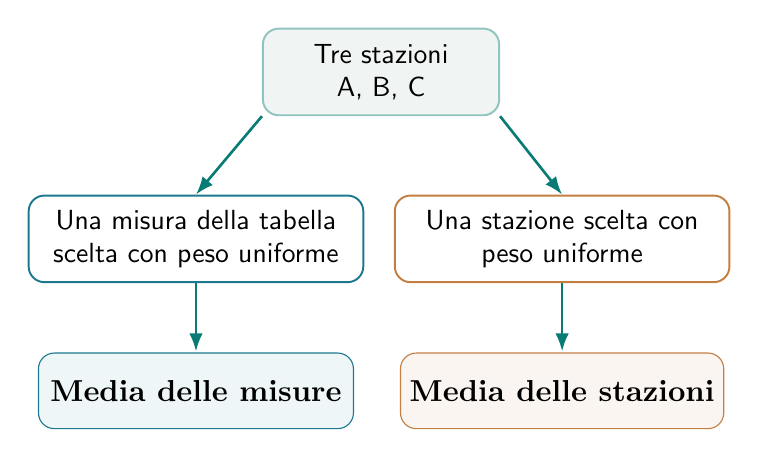
\begin{tikzpicture}[x=1cm,y=1cm]
 \node[pFlow,fill=GeoTint,minimum width=3cm,minimum height=1.1cm] (d) at (5.0,5.35) {Tre stazioni\\A, B, C};
 \node[pFlow,minimum width=4.25cm,minimum height=1.1cm,draw=GeoA] (m) at (2.65,3.23) {Una misura della tabella\\scelta con peso uniforme};
 \node[pFlow,minimum width=4.25cm,minimum height=1.1cm,draw=GeoB] (s) at (7.3,3.23) {Una stazione scelta con\\peso uniforme};
 \draw[pEdge] (d.south west) -- (m.north);\draw[pEdge] (d.south east) -- (s.north);
 \node[draw=GeoA,fill=GeoA!7,rounded corners=2mm,minimum width=4cm,minimum height=.96cm,
  font=\bfseries\fontsize{10.5}{13}\selectfont,align=center] at (2.65,1.3) {Media delle misure};
 \node[draw=GeoB,fill=GeoB!8,rounded corners=2mm,minimum width=4cm,minimum height=.96cm,
  font=\bfseries\fontsize{10.5}{13}\selectfont,align=center] at (7.3,1.3) {Media delle stazioni};
 \draw[pEdge] (m.south)--(2.65,1.80);\draw[pEdge] (s.south)--(7.3,1.80);
\end{tikzpicture}
\PInfo{La differenza fra le due sintesi dipende dai pesi assegnati ai gruppi, non da un errore del programma.}

\end{minipage}%
\end{lrbox}
\typeout{FULLBOX:017:L:\the\ht\PilotLeftBox:\the\dp\PilotLeftBox}
\begin{lrbox}{\PilotRightBox}%
\begin{minipage}[t]{7.55cm}\raggedright\color{Ink}\fontsize{11.3}{14.8}\selectfont

\PLabel{Quantità teorica e stima}
\PBody{L'\textbf{estimando} è la quantità definita dalla domanda. Lo \textbf{stimatore} è la regola che la stima a partire dai dati.}
\[\theta_w=\sum_{g=1}^{G}w_g\mu_g,
\qquad \widehat\theta_w=\sum_{g=1}^{G}w_g\bar x_g.\]
\PSmall{\(\mu_g\): media della stazione nel modello; \(\bar x_g\): media osservata. I pesi soddisfano \(\sum_g w_g=1\).}
\vspace{2mm}\PInfo{Per una misura scelta fra le righe, \(w_g=n_g/N\). Per una stazione scelta fra le tre, \(w_g=1/G\). Le due domande assegnano pesi differenti.}

\end{minipage}%
\end{lrbox}
\typeout{FULLBOX:017:R:\the\ht\PilotRightBox:\the\dp\PilotRightBox}
\begin{frame}[plain]\hypertarget{slide17}{}
\bookmark[level=1,page=17]{Quantità di interesse: due domande diverse}
\begin{tikzpicture}[remember picture,overlay]
\PilotChrome{Quantità di interesse: due domande diverse}{TERRA 01 · TEORIA}{17}{La definizione dell’estimando determina i pesi; il calcolo viene dopo.}
\node[anchor=north west,inner sep=0] at ([xshift=0.96cm,yshift=-2.13cm]current page.north west) {\usebox{\PilotLeftBox}};
\node[anchor=north west,inner sep=0] at ([xshift=11.52cm,yshift=-2.13cm]current page.north west) {\usebox{\PilotRightBox}};
\end{tikzpicture}
\end{frame}

% SLIDE 018 | Una tabella, due livelli di analisi | REVISIONE COMPLETA
\begin{lrbox}{\PilotLeftBox}%
\begin{minipage}[t]{10.05cm}\raggedright\color{Ink}\fontsize{11.3}{14.8}\selectfont
\PLabel{La gerarchia osservata nel modello}
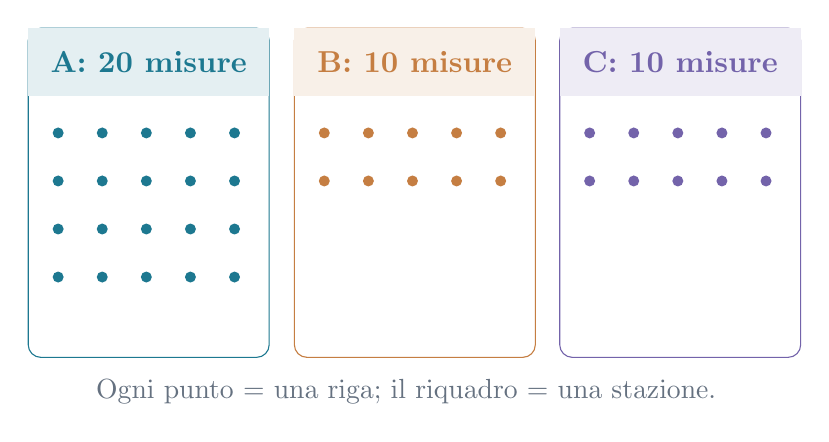
\begin{tikzpicture}[x=1cm,y=1cm]
 \foreach \sx/\name/\num/\col in {.20/A/20/GeoA,3.58/B/10/GeoB,6.95/C/10/GeoC}{
  \draw[rounded corners=1.6mm,draw=\col,fill=white] (\sx,.86) rectangle ++(3.06,4.18);
  \fill[\col!12] (\sx,4.18) rectangle ++(3.06,.86);
  \node[color=\col,font=\bfseries\fontsize{11}{13}\selectfont] at (\sx+1.53,4.61) {\name : \num\ misure};
  \ifnum\num=20
    \foreach \rr in {0,1,2,3}{\foreach \cc in {0,1,2,3,4}{\node[circle,fill=\col,inner sep=1.4pt] at (\sx+.38+\cc*.56,3.71-\rr*.61) {};}}
  \else
    \foreach \rr in {0,1}{\foreach \cc in {0,1,2,3,4}{\node[circle,fill=\col,inner sep=1.4pt] at (\sx+.38+\cc*.56,3.71-\rr*.61) {};}}
  \fi
 }
 \node[font=\fontsize{10}{12.6}\selectfont,color=Muted] at (5.0,.42) {Ogni punto = una riga; il riquadro = una stazione.};
\end{tikzpicture}

\end{minipage}%
\end{lrbox}
\typeout{FULLBOX:018:L:\the\ht\PilotLeftBox:\the\dp\PilotLeftBox}
\begin{lrbox}{\PilotRightBox}%
\begin{minipage}[t]{7.55cm}\raggedright\color{Ink}\fontsize{11.3}{14.8}\selectfont

\PLabel{Contare righe e gruppi}
\[G=3,\qquad N=\sum_g n_g=40.\]
\PCode{R · conteggi nell'anteprima}{18_conteggi.R}
\PSmall{\texttt{terra} è stato caricato da \texttt{setup.R}. \texttt{table()} restituisce 20, 10, 10; \texttt{nlevels()} conta i tre livelli della variabile categoriale.}

\end{minipage}%
\end{lrbox}
\typeout{FULLBOX:018:R:\the\ht\PilotRightBox:\the\dp\PilotRightBox}
\begin{frame}[plain]\hypertarget{slide18}{}
\bookmark[level=1,page=18]{Una tabella, due livelli di analisi}
\begin{tikzpicture}[remember picture,overlay]
\PilotChrome{Una tabella, due livelli di analisi}{TERRA 01 · GERARCHIA}{18}{Lo stesso dataset può essere letto per misura oppure per stazione: la domanda individua il livello pertinente.}
\node[anchor=north west,inner sep=0] at ([xshift=0.96cm,yshift=-2.13cm]current page.north west) {\usebox{\PilotLeftBox}};
\node[anchor=north west,inner sep=0] at ([xshift=11.52cm,yshift=-2.13cm]current page.north west) {\usebox{\PilotRightBox}};
\end{tikzpicture}
\end{frame}

% SLIDE 019 | Due medie: stessi dati, pesi differenti | REVISIONE COMPLETA
\begin{lrbox}{\PilotLeftBox}%
\begin{minipage}[t]{10.05cm}\raggedright\color{Ink}\fontsize{11.3}{14.8}\selectfont
\PLabel{Ripartizione dei pesi fra stazioni}
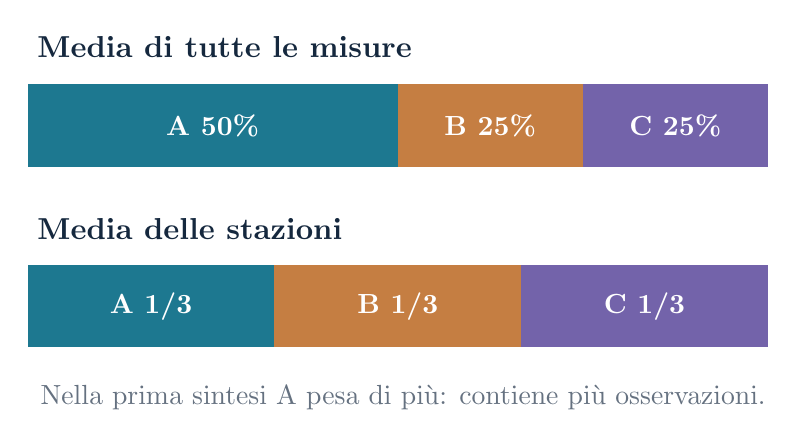
\begin{tikzpicture}[x=1cm,y=1cm]
 \node[anchor=west,font=\bfseries\fontsize{11}{14}\selectfont,color=Navy] at (.3,5.15) {Media di tutte le misure};
 \fill[GeoA] (.3,3.63) rectangle (5.0,4.68);
 \fill[GeoB] (5.0,3.63) rectangle (7.35,4.68);
 \fill[GeoC] (7.35,3.63) rectangle (9.7,4.68);
 \foreach \x/\lab in {2.65/{A 50\%},6.175/{B 25\%},8.525/{C 25\%}}\node[color=white,font=\bfseries\fontsize{10}{12}\selectfont] at (\x,4.15) {\lab};
 \node[anchor=west,font=\bfseries\fontsize{11}{14}\selectfont,color=Navy] at (.3,2.85) {Media delle stazioni};
 \fill[GeoA] (.3,1.34) rectangle (3.433,2.39);
 \fill[GeoB] (3.433,1.34) rectangle (6.566,2.39);
 \fill[GeoC] (6.566,1.34) rectangle (9.7,2.39);
 \foreach \x/\lab in {1.866/{A 1/3},5.0/{B 1/3},8.133/{C 1/3}}\node[color=white,font=\bfseries\fontsize{10}{12}\selectfont] at (\x,1.86) {\lab};
 \node[anchor=west,font=\fontsize{9.6}{12.8}\selectfont,color=Muted] at (.34,.7) {Nella prima sintesi A pesa di più: contiene più osservazioni.};
\end{tikzpicture}

\end{minipage}%
\end{lrbox}
\typeout{FULLBOX:019:L:\the\ht\PilotLeftBox:\the\dp\PilotLeftBox}
\begin{lrbox}{\PilotRightBox}%
\begin{minipage}[t]{7.55cm}\raggedright\color{Ink}\fontsize{11.3}{14.8}\selectfont
\PLabel{Scrittura matematica}
\[\bar{x}_g=\frac{1}{n_g}\sum_{i=1}^{n_g}x_{ig},\qquad N=\sum_g n_g.\]
\vspace{-1mm}
\[\bar{x}_{\mathrm{mis}}=\sum_{g=1}^{G}\underbrace{\frac{n_g}{N}}_{w_g}\bar{x}_g\]
\vspace{-1mm}
\[\bar{x}_{\mathrm{st}}=\sum_{g=1}^{G}\frac{1}{G}\bar{x}_g.\]
\PInfo{Entrambi i sistemi di pesi sommano a 1. Con \(n_1=\dots=n_G\), le due statistiche coincidono sugli stessi dati.}

\end{minipage}%
\end{lrbox}
\typeout{FULLBOX:019:R:\the\ht\PilotRightBox:\the\dp\PilotRightBox}
\begin{frame}[plain]\hypertarget{slide19}{}
\bookmark[level=1,page=19]{Due medie: stessi dati, pesi differenti}
\begin{tikzpicture}[remember picture,overlay]
\PilotChrome{Due medie: stessi dati, pesi differenti}{TERRA 01 · FORMULE}{19}{Il peso della stazione è \(n_g/N\) nella media delle misure e \(1/G\) nella media delle stazioni.}
\node[anchor=north west,inner sep=0] at ([xshift=0.96cm,yshift=-2.13cm]current page.north west) {\usebox{\PilotLeftBox}};
\node[anchor=north west,inner sep=0] at ([xshift=11.52cm,yshift=-2.13cm]current page.north west) {\usebox{\PilotRightBox}};
\end{tikzpicture}
\end{frame}

% SLIDE 020 | Un esempio numerico prima della simulazione | REVISIONE COMPLETA
\begin{lrbox}{\PilotLeftBox}%
\begin{minipage}[t]{10.05cm}\raggedright\color{Ink}\fontsize{11.3}{14.8}\selectfont
\PLabel{Medie di stazione fissate (esempio teorico)}
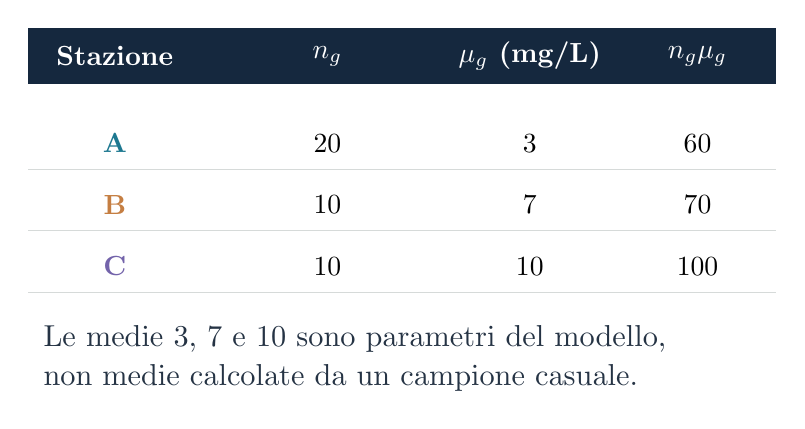
\begin{tikzpicture}[x=1cm,y=1cm]
 \fill[Navy] (.25,4.66) rectangle (9.75,5.37);
 \foreach \x/\t in {1.35/{Stazione},4.05/{$n_g$},6.62/{$\mu_g$ (mg/L)},8.75/{$n_g\mu_g$}} {
  \node[color=white,font=\bfseries\fontsize{10.2}{12}\selectfont] at (\x,5.01) {\t};}
 \foreach \y/\st/\n/\mu/\prod/\col in {3.90/A/20/3/60/GeoA,3.12/B/10/7/70/GeoB,2.34/C/10/10/100/GeoC}{
  \fill[white] (.25,\y-.33) rectangle (9.75,\y+.34);
  \draw[Rule] (.25,\y-.33)--(9.75,\y-.33);
  \node[color=\col,font=\bfseries] at (1.35,\y) {\st};
  \node at (4.05,\y) {\n};\node at (6.62,\y) {\mu};\node at (8.75,\y) {\prod};}
 \node[anchor=west,font=\fontsize{10.5}{13}\selectfont,color=Ink] at (.32,1.42) {Le medie 3, 7 e 10 sono parametri del modello,};
 \node[anchor=west,font=\fontsize{10.5}{13}\selectfont,color=Ink] at (.32,.92) {non medie calcolate da un campione casuale.};
\end{tikzpicture}

\end{minipage}%
\end{lrbox}
\typeout{FULLBOX:020:L:\the\ht\PilotLeftBox:\the\dp\PilotLeftBox}
\begin{lrbox}{\PilotRightBox}%
\begin{minipage}[t]{7.55cm}\raggedright\color{Ink}\fontsize{11.3}{14.8}\selectfont
\PLabel{Il peso modifica la sintesi}
\[\bar\mu_{\mathrm{mis}}=\frac{20(3)+10(7)+10(10)}{40}\]
\vspace{-2mm}
\[\boxed{\bar\mu_{\mathrm{mis}}=5{,}75\ \mathrm{mg/L}}\]
\[\bar\mu_{\mathrm{st}}=\frac{3+7+10}{3}\]
\vspace{-2mm}
\[\boxed{\bar\mu_{\mathrm{st}}\simeq6{,}67\ \mathrm{mg/L}}\]
\PInfo{A ha la concentrazione minore ma metà delle misure: per questo la prima sintesi è inferiore alla seconda.}

\end{minipage}%
\end{lrbox}
\typeout{FULLBOX:020:R:\the\ht\PilotRightBox:\the\dp\PilotRightBox}
\begin{frame}[plain]\hypertarget{slide20}{}
\bookmark[level=1,page=20]{Un esempio numerico prima della simulazione}
\begin{tikzpicture}[remember picture,overlay]
\PilotChrome{Un esempio numerico prima della simulazione}{TERRA 01 · CALCOLO}{20}{L’esempio isola l’effetto dei pesi; nella simulazione si aggiunge la variabilità dei valori estratti.}
\node[anchor=north west,inner sep=0] at ([xshift=0.96cm,yshift=-2.13cm]current page.north west) {\usebox{\PilotLeftBox}};
\node[anchor=north west,inner sep=0] at ([xshift=11.52cm,yshift=-2.13cm]current page.north west) {\usebox{\PilotRightBox}};
\end{tikzpicture}
\end{frame}

% SLIDE 021 | Più misure in A: valori attesi delle due medie | REVISIONE COMPLETA
\begin{lrbox}{\PilotLeftBox}%
\begin{minipage}[t]{10.05cm}\raggedright\color{Ink}\fontsize{11.3}{14.8}\selectfont

\PLabel{Varia $n_A$; restano fissi i parametri del modello}
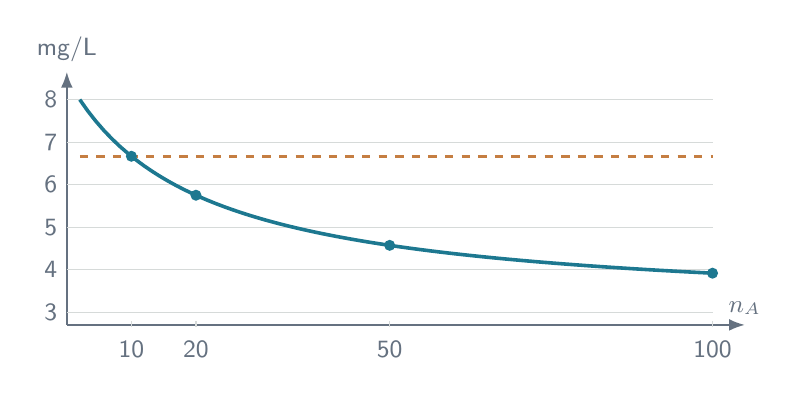
\begin{tikzpicture}[x=.082cm,y=.54cm]
\draw[pAxis](0,2.7)--(105,2.7)node[above,pNote]{$n_A$};
\draw[pAxis](0,2.7)--(0,8.65)node[above,pNote]{mg/L};
\foreach \xx in {10,20,50,100}{\draw[Rule](\xx,2.65)--(\xx,2.8);\node[pNote,below]at(\xx,2.55){\xx};}
\foreach \yy in {3,4,5,6,7,8}{\draw[Rule](0,\yy)--(100,\yy);\node[pNote,left]at(0,\yy){\yy};}
\draw[GeoA,line width=1.3pt,domain=2:100,samples=80]plot(\x,{(3*\x+170)/(\x+20)});
\draw[GeoB,line width=1.1pt,dashed](2,{20/3})--(100,{20/3});
\foreach \xx in {10,20,50,100}{\fill[GeoA](\xx,{(3*\xx+170)/(\xx+20)})circle(2pt);}
\end{tikzpicture}
\PSmall{\textcolor{GeoA}{Linea continua}: media delle misure. \textcolor{GeoB}{Linea tratteggiata}: media delle stazioni. Valori attesi, prima di estrarre il campione.}
\[\mathbb E(\bar X_m)=\frac{3n_A+170}{n_A+20},\qquad
\mathbb E(\bar X_s)=\frac{20}{3}.\]

\end{minipage}%
\end{lrbox}
\typeout{FULLBOX:021:L:\the\ht\PilotLeftBox:\the\dp\PilotLeftBox}
\begin{lrbox}{\PilotRightBox}%
\begin{minipage}[t]{7.55cm}\raggedright\color{Ink}\fontsize{11.3}{14.8}\selectfont

\PCode{R · calcolo teorico per quattro scenari}{21_attese.R}
\PInfo{Con uguali numerosità, le due medie coincidono esattamente sullo stesso campione. Cambiando \(n_A\), cambia il peso attribuito ad A nella media delle misure.}

\end{minipage}%
\end{lrbox}
\typeout{FULLBOX:021:R:\the\ht\PilotRightBox:\the\dp\PilotRightBox}
\begin{frame}[plain]\hypertarget{slide21}{}
\bookmark[level=1,page=21]{Più misure in A: valori attesi delle due medie}
\begin{tikzpicture}[remember picture,overlay]
\PilotChrome{Più misure in A: valori attesi delle due medie}{TERRA 01 · EFFETTO DEI PESI}{21}{La media delle stazioni resta costante in valore atteso; quella calcolata su un singolo campione può variare.}
\node[anchor=north west,inner sep=0] at ([xshift=0.96cm,yshift=-2.13cm]current page.north west) {\usebox{\PilotLeftBox}};
\node[anchor=north west,inner sep=0] at ([xshift=11.52cm,yshift=-2.13cm]current page.north west) {\usebox{\PilotRightBox}};
\end{tikzpicture}
\end{frame}

% SLIDE 022 | Campioni simulati e riproducibilità | REVISIONE COMPLETA
\begin{lrbox}{\PilotLeftBox}%
\begin{minipage}[t]{10.05cm}\raggedright\color{Ink}\fontsize{11.3}{14.8}\selectfont

\PLabel{Tre distribuzioni normali con dispersione comune}
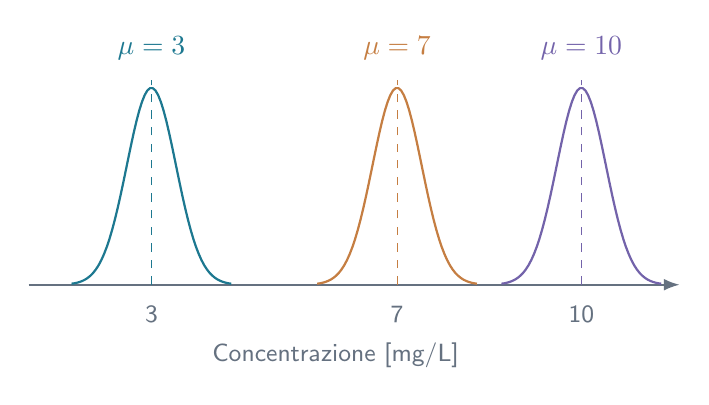
\begin{tikzpicture}[x=.78cm,y=1cm]
\draw[pAxis](1,.5)--(11.6,.5);
\foreach \mval/\col in {3/GeoA,7/GeoB,10/GeoC}{
 \draw[\col,thick,domain=-1.3:1.3,samples=60,variable=\u] plot({\mval+\u},{.5+2.5*exp(-.5*(\u/.4)^2)});
 \draw[\col,dashed](\mval,.5)--(\mval,3.1);
 \node[pLabel,text=\col]at(\mval,3.5){$\mu=\mval$};
 \node[pNote,below]at(\mval,.35){\mval};}
\node[pNote]at(6,-.4){Concentrazione [mg/L]};
\end{tikzpicture}
\[X_{ig}\sim\mathcal N(\mu_g,\sigma^2),\quad \sigma=0{,}4\ \mathrm{mg/L}.\]
\PSmall{Le estrazioni del modello sono indipendenti. La dispersione delle singole misure è \(\sigma\); l'errore standard della media è \(\operatorname{SE}(\bar X_g)=\sigma/\sqrt{n_g}\).}

\end{minipage}%
\end{lrbox}
\typeout{FULLBOX:022:L:\the\ht\PilotLeftBox:\the\dp\PilotLeftBox}
\begin{lrbox}{\PilotRightBox}%
\begin{minipage}[t]{7.55cm}\raggedright\color{Ink}\fontsize{11.3}{14.8}\selectfont

\PCode{R · estrarre un campione riproducibile}{22_simulazione.R}
\PSmall{\texttt{set.seed()} fissa lo stato iniziale del generatore. \texttt{rnorm()} estrae valori normali usando numerosità, media e deviazione standard indicate.}
\vspace{2mm}\PInfo{A seme fisso, cambiare \(n_A\) sposta anche i numeri della sequenza usati per B e C. Le loro medie osservate possono cambiare.}

\end{minipage}%
\end{lrbox}
\typeout{FULLBOX:022:R:\the\ht\PilotRightBox:\the\dp\PilotRightBox}
\begin{frame}[plain]\hypertarget{slide22}{}
\bookmark[level=1,page=22]{Campioni simulati e riproducibilità}
\begin{tikzpicture}[remember picture,overlay]
\PilotChrome{Campioni simulati e riproducibilità}{TERRA 01 · GENERATORE}{22}{Il seme controlla la sequenza pseudo-casuale, non elimina la variabilità campionaria fra scenari.}
\node[anchor=north west,inner sep=0] at ([xshift=0.96cm,yshift=-2.13cm]current page.north west) {\usebox{\PilotLeftBox}};
\node[anchor=north west,inner sep=0] at ([xshift=11.52cm,yshift=-2.13cm]current page.north west) {\usebox{\PilotRightBox}};
\end{tikzpicture}
\end{frame}

% SLIDE 023 | Costruire in R i dati di Terra 01 | REVISIONE COMPLETA
\begin{lrbox}{\PilotLeftBox}%
\begin{minipage}[t]{10.05cm}\raggedright\color{Ink}\fontsize{11.3}{14.8}\selectfont

\PLabel{Dal modello alla tabella simulata}
\PCode{R · lo stesso generatore di Terra01}{23_costruzione.R}
\PSmall{Il punto è il separatore decimale nel codice. In \texttt{rnorm(n, mean, sd)}, il terzo argomento è la deviazione standard, non la varianza.}

\end{minipage}%
\end{lrbox}
\typeout{FULLBOX:023:L:\the\ht\PilotLeftBox:\the\dp\PilotLeftBox}
\begin{lrbox}{\PilotRightBox}%
\begin{minipage}[t]{7.55cm}\raggedright\color{Ink}\fontsize{11.3}{14.8}\selectfont

\PLabel{Accoppiare etichette e valori}
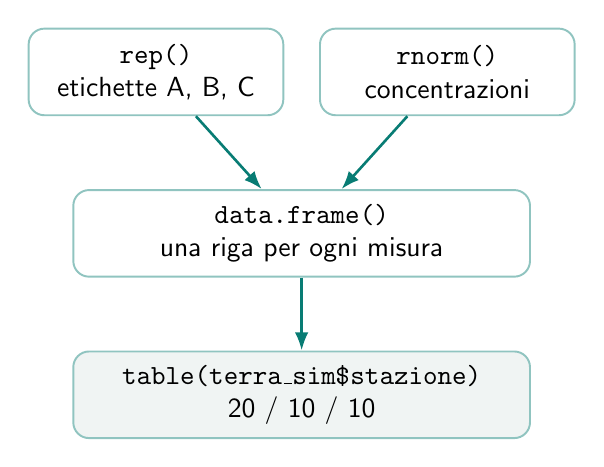
\begin{tikzpicture}[x=1cm,y=1cm]
\node[pFlow,minimum width=3.1cm,text width=3cm] (g) at(1.8,5.8){\texttt{rep()}\\etichette A, B, C};
\node[pFlow,minimum width=3.1cm,text width=3cm] (v) at(5.5,5.8){\texttt{rnorm()}\\concentrazioni};
\node[pFlow,minimum width=5.8cm] (t) at(3.65,3.75){\texttt{data.frame()}\\una riga per ogni misura};
\draw[pEdge](g)--(t);\draw[pEdge](v)--(t);
\node[pFlow,minimum width=5.8cm,fill=GeoTint] (c) at(3.65,1.7){\texttt{table(terra\_sim\$stazione)}\\20 / 10 / 10};
\draw[pEdge](t)--(c);
\end{tikzpicture}
\PSmall{I due vettori hanno entrambi \(n_A+20\) elementi. \texttt{terra\_sim} conserva il campione appena generato.}

\end{minipage}%
\end{lrbox}
\typeout{FULLBOX:023:R:\the\ht\PilotRightBox:\the\dp\PilotRightBox}
\begin{frame}[plain]\hypertarget{slide23}{}
\bookmark[level=1,page=23]{Costruire in R i dati di Terra 01}
\begin{tikzpicture}[remember picture,overlay]
\PilotChrome{Costruire in R i dati di Terra 01}{TERRA 01 · CODICE}{23}{La sintassi di R traduce una struttura statistica: per ogni misura vengono conservati gruppo e valore.}
\node[anchor=north west,inner sep=0] at ([xshift=0.96cm,yshift=-2.13cm]current page.north west) {\usebox{\PilotLeftBox}};
\node[anchor=north west,inner sep=0] at ([xshift=11.52cm,yshift=-2.13cm]current page.north west) {\usebox{\PilotRightBox}};
\end{tikzpicture}
\end{frame}

% SLIDE 024 | Calcolare le due medie in R | REVISIONE COMPLETA
\begin{lrbox}{\PilotLeftBox}%
\begin{minipage}[t]{10.05cm}\raggedright\color{Ink}\fontsize{11.3}{14.8}\selectfont

\PLabel{Dalle misure alle medie di gruppo}
\PCode{R · medie e pesi coerenti}{24_medie.R}
\PInfo{\texttt{m} contiene tre medie, \texttt{n} le tre numerosità. I loro nomi A, B, C permettono di allineare i pesi. \texttt{weighted.mean()} deve ritrovare la media di tutte le misure.}

\end{minipage}%
\end{lrbox}
\typeout{FULLBOX:024:L:\the\ht\PilotLeftBox:\the\dp\PilotLeftBox}
\begin{lrbox}{\PilotRightBox}%
\begin{minipage}[t]{7.55cm}\raggedright\color{Ink}\fontsize{11.3}{14.8}\selectfont
\PLabel{Anteprima reale del laboratorio (seme 17)}
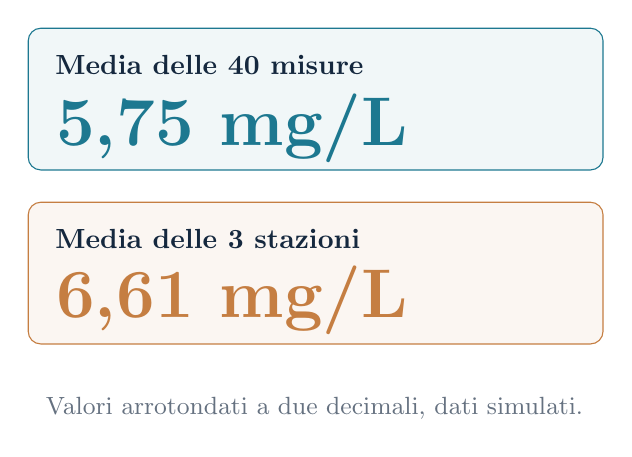
\begin{tikzpicture}[x=1cm,y=1cm]
 \draw[rounded corners=1.6mm,draw=GeoA,fill=GeoA!6] (.1,3.93) rectangle (7.4,5.73);
 \node[anchor=west,color=Navy,font=\bfseries\fontsize{10.2}{12}\selectfont] at (.32,5.27) {Media delle 40 misure};
 \node[anchor=west,color=GeoA,font=\bfseries\fontsize{24}{27}\selectfont] at (.33,4.46) {5,75 mg/L};
 \draw[rounded corners=1.6mm,draw=GeoB,fill=GeoB!7] (.1,1.72) rectangle (7.4,3.52);
 \node[anchor=west,color=Navy,font=\bfseries\fontsize{10.2}{12}\selectfont] at (.32,3.05) {Media delle 3 stazioni};
 \node[anchor=west,color=GeoB,font=\bfseries\fontsize{24}{27}\selectfont] at (.33,2.27) {6,61 mg/L};
 \node[anchor=west,color=Muted,font=\fontsize{9.1}{12}\selectfont] at (.2,.9) {Valori arrotondati a due decimali, dati simulati.};
\end{tikzpicture}
\PSmall{6,61 mg/L è una stima dal campione; 6,67 mg/L è la media teorica delle tre stazioni.}

\end{minipage}%
\end{lrbox}
\typeout{FULLBOX:024:R:\the\ht\PilotRightBox:\the\dp\PilotRightBox}
\begin{frame}[plain]\hypertarget{slide24}{}
\bookmark[level=1,page=24]{Calcolare le due medie in R}
\begin{tikzpicture}[remember picture,overlay]
\PilotChrome{Calcolare le due medie in R}{TERRA 01 · CODICE E OUTPUT}{24}{La stima dipende dai dati estratti; il valore teorico dipende dai parametri del generatore.}
\node[anchor=north west,inner sep=0] at ([xshift=0.96cm,yshift=-2.13cm]current page.north west) {\usebox{\PilotLeftBox}};
\node[anchor=north west,inner sep=0] at ([xshift=11.52cm,yshift=-2.13cm]current page.north west) {\usebox{\PilotRightBox}};
\end{tikzpicture}
\end{frame}

% SLIDE 025 | Leggere boxplot e medie di stazione | REVISIONE COMPLETA
\begin{lrbox}{\PilotLeftBox}%
\begin{minipage}[t]{10.05cm}\raggedright\color{Ink}\fontsize{11.3}{14.8}\selectfont

\PLabel{Elementi di un boxplot}
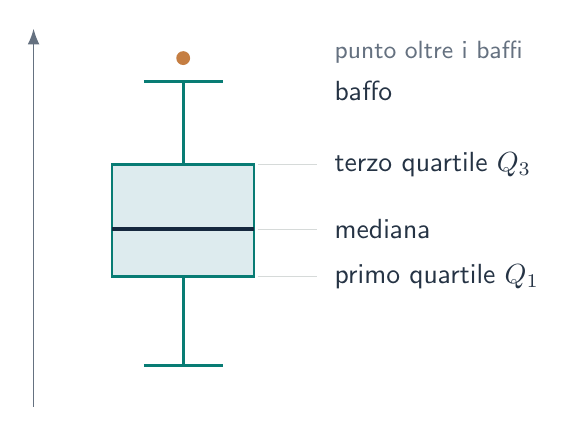
\begin{tikzpicture}[x=1cm,y=.75cm]
\draw[pAxis](.8,.3)--(.8,6.7);
\draw[Classical,line width=1pt](2.7,1)--(2.7,2.5);
\draw[Classical,line width=1pt](2.7,4.4)--(2.7,5.8);
\draw[Classical,line width=1pt](2.2,1)--(3.2,1);
\draw[Classical,line width=1pt](2.2,5.8)--(3.2,5.8);
\filldraw[fill=GeoA!15,draw=Classical,line width=.8pt](1.8,2.5)rectangle(3.6,4.4);
\draw[Navy,line width=1.5pt](1.8,3.3)--(3.6,3.3);
\fill[GeoB](2.7,6.2)circle(2.5pt);
\foreach \yy/\lab in {2.5/{primo quartile $Q_1$},3.3/{mediana},4.4/{terzo quartile $Q_3$}}{
\draw[Rule](3.65,\yy)--(4.4,\yy);\node[pLabel,anchor=west]at(4.5,\yy){\lab};}
\node[pLabel,anchor=west]at(4.5,5.65){baffo};\node[pNote,anchor=west]at(4.5,6.3){punto oltre i baffi};
\end{tikzpicture}
\PSmall{Schema illustrativo. Nel boxplot standard i baffi arrivano ai valori estremi entro \(1{,}5\,\mathrm{IQR}\) dai bordi della scatola, con \(\mathrm{IQR}=Q_3-Q_1\).}

\end{minipage}%
\end{lrbox}
\typeout{FULLBOX:025:L:\the\ht\PilotLeftBox:\the\dp\PilotLeftBox}
\begin{lrbox}{\PilotRightBox}%
\begin{minipage}[t]{7.55cm}\raggedright\color{Ink}\fontsize{11.3}{14.8}\selectfont

\PCode{R · boxplot e medie separate}{25_boxplot.R}
\PSmall{\texttt{valore \textasciitilde{} stazione} separa i gruppi. Le medie dell'anteprima sono circa 3,177; 7,062; 9,576 mg/L.}
\PInfo{La linea interna è la mediana. La larghezza standard non indica la numerosità. Un punto oltre i baffi richiede verifica.}

\end{minipage}%
\end{lrbox}
\typeout{FULLBOX:025:R:\the\ht\PilotRightBox:\the\dp\PilotRightBox}
\begin{frame}[plain]\hypertarget{slide25}{}
\bookmark[level=1,page=25]{Leggere boxplot e medie di stazione}
\begin{tikzpicture}[remember picture,overlay]
\PilotChrome{Leggere boxplot e medie di stazione}{TERRA 01 · LEGGERE IL GRAFICO}{25}{Il boxplot riassume mediana e dispersione; per interpretare le medie e le numerosità occorrono calcoli separati.}
\node[anchor=north west,inner sep=0] at ([xshift=0.96cm,yshift=-2.13cm]current page.north west) {\usebox{\PilotLeftBox}};
\node[anchor=north west,inner sep=0] at ([xshift=11.52cm,yshift=-2.13cm]current page.north west) {\usebox{\PilotRightBox}};
\end{tikzpicture}
\end{frame}

% SLIDE 026 | Terra01: eseguire e confrontare gli scenari | REVISIONE COMPLETA
\begin{lrbox}{\PilotLeftBox}%
\begin{minipage}[t]{10.05cm}\raggedright\color{Ink}\fontsize{11.3}{14.8}\selectfont

\PLabel{Impostazioni e risultato}
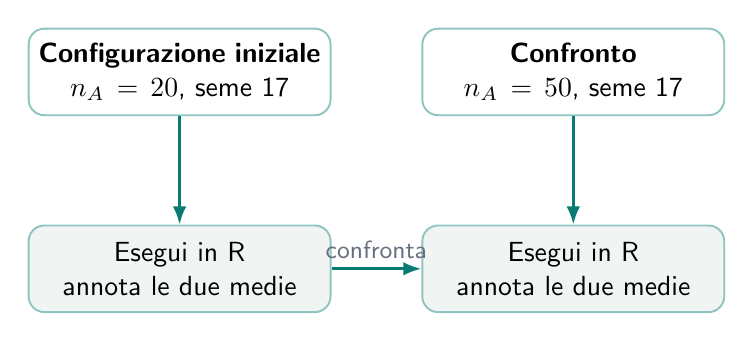
\begin{tikzpicture}[x=1cm,y=1cm]
\node[pFlow,minimum width=3.8cm,text width=3.6cm] (a) at(2.2,4.8){\textbf{Configurazione iniziale}\\$n_A=20$, seme 17};
\node[pFlow,minimum width=3.8cm,text width=3.6cm] (b) at(7.2,4.8){\textbf{Confronto}\\$n_A=50$, seme 17};
\node[pFlow,minimum width=3.8cm,text width=3.6cm,fill=GeoTint] (ar) at(2.2,2.3){Esegui in R\\annota le due medie};
\node[pFlow,minimum width=3.8cm,text width=3.6cm,fill=GeoTint] (br) at(7.2,2.3){Esegui in R\\annota le due medie};
\draw[pEdge](a)--(ar);\draw[pEdge](b)--(br);
\draw[pEdge](ar)--node[above,pNote]{confronta}(br);
\end{tikzpicture}
\PBody{Aprire \href{https://marzione00.github.io/Lab_Geo/\#laboratorio/m01-estimando}{Terra · 01 · Definire la quantità di interesse}. Attendere \textbf{CALCOLO R COMPLETATO} prima di leggere gli indicatori.}

\end{minipage}%
\end{lrbox}
\typeout{FULLBOX:026:L:\the\ht\PilotLeftBox:\the\dp\PilotLeftBox}
\begin{lrbox}{\PilotRightBox}%
\begin{minipage}[t]{7.55cm}\raggedright\color{Ink}\fontsize{11.3}{14.8}\selectfont

\PLabel{Che cosa salvare}
\PBody{\textbf{Conserva scenario A/B}: mantiene due configurazioni da confrontare.\\[2mm]
\textbf{Scarica dati CSV}: salva le osservazioni.\\[2mm]
\textbf{Esporta configurazione}: salva i parametri dell'esperimento.}
\vspace{3mm}\PInfo{\emph{Formalismo e codice} mostra lo script. \emph{Nuovo campione} cambia il seme. Gli scenari A/B sono configurazioni; le stazioni A, B e C sono gruppi di misure.}

\end{minipage}%
\end{lrbox}
\typeout{FULLBOX:026:R:\the\ht\PilotRightBox:\the\dp\PilotRightBox}
\begin{frame}[plain]\hypertarget{slide26}{}
\bookmark[level=1,page=26]{Terra01: eseguire e confrontare gli scenari}
\begin{tikzpicture}[remember picture,overlay]
\PilotChrome{Terra01: eseguire e confrontare gli scenari}{LABORATORIO NEL BROWSER}{26}{Per ricostruire un confronto, conservare dati, numerosità, seme e definizione delle due medie.}
\node[anchor=north west,inner sep=0] at ([xshift=0.96cm,yshift=-2.13cm]current page.north west) {\usebox{\PilotLeftBox}};
\node[anchor=north west,inner sep=0] at ([xshift=11.52cm,yshift=-2.13cm]current page.north west) {\usebox{\PilotRightBox}};
\end{tikzpicture}
\end{frame}

% SLIDE 027 | Esercizio: quattro numerosità nella stazione A | REVISIONE COMPLETA
\begin{lrbox}{\PilotLeftBox}%
\begin{minipage}[t]{10.05cm}\raggedright\color{Ink}\fontsize{11.3}{14.8}\selectfont

\PLabel{Prima una previsione, poi il calcolo}
\PBody{Mantenere il seme a 17 e dieci misure in B e C. Prevedere come cambia la media delle misure, poi compilare la tabella.}
\vspace{3mm}\renewcommand{\arraystretch}{1.5}
\begin{tabular}{@{}rrrr@{}}\toprule
$n_A$&$N$&Media misure&Media stazioni\\\midrule
10&30&\rule{1.8cm}{.3pt}&\rule{1.8cm}{.3pt}\\
20&40&\rule{1.8cm}{.3pt}&\rule{1.8cm}{.3pt}\\
50&70&\rule{1.8cm}{.3pt}&\rule{1.8cm}{.3pt}\\
100&120&\rule{1.8cm}{.3pt}&\rule{1.8cm}{.3pt}\\\bottomrule
\end{tabular}
\PSmall{Concentrazioni in mg/L. Riportare i risultati dei campioni generati; confrontarli con i valori teorici della slide 21.}

\end{minipage}%
\end{lrbox}
\typeout{FULLBOX:027:L:\the\ht\PilotLeftBox:\the\dp\PilotLeftBox}
\begin{lrbox}{\PilotRightBox}%
\begin{minipage}[t]{7.55cm}\raggedright\color{Ink}\fontsize{11.3}{14.8}\selectfont

\PLabel{Domande per la discussione}
\PBody{1. Perché con dieci misure per stazione le due medie coincidono?\\[2mm]
2. Quale peso assume A quando \(n_A=100\)?\\[2mm]
3. Perché la media delle stazioni può cambiare anche a seme fisso?\\[2mm]
4. Quale media risponde alla domanda su una stazione scelta con uguale probabilità?}
\vspace{3mm}\PInfo{Ripetere il confronto con un altro seme. Distinguere il cambiamento sistematico dovuto ai pesi dalle fluttuazioni del singolo campione.}

\end{minipage}%
\end{lrbox}
\typeout{FULLBOX:027:R:\the\ht\PilotRightBox:\the\dp\PilotRightBox}
\begin{frame}[plain]\hypertarget{slide27}{}
\bookmark[level=1,page=27]{Esercizio: quattro numerosità nella stazione A}
\begin{tikzpicture}[remember picture,overlay]
\PilotChrome{Esercizio: quattro numerosità nella stazione A}{TERRA 01 · ATTIVITÀ}{27}{Consegna: tabella, previsione confrontata con i risultati e una conclusione che dichiari la quantità stimata.}
\node[anchor=north west,inner sep=0] at ([xshift=0.96cm,yshift=-2.13cm]current page.north west) {\usebox{\PilotLeftBox}};
\node[anchor=north west,inner sep=0] at ([xshift=11.52cm,yshift=-2.13cm]current page.north west) {\usebox{\PilotRightBox}};
\end{tikzpicture}
\end{frame}

% SLIDE 028 | Una conclusione coerente con la domanda | REVISIONE COMPLETA
\begin{lrbox}{\PilotLeftBox}%
\begin{minipage}[t]{10.05cm}\raggedright\color{Ink}\fontsize{11.3}{14.8}\selectfont

\PLabel{Un esempio sul campione iniziale}
\PBody{«Con 20 misure in A e 10 in B e C, la media delle 40 concentrazioni è 5,75 mg/L. La media delle tre medie di stazione è 6,61 mg/L.\par\vspace{3mm}
Nel primo calcolo A riceve il 50\% del peso; nel secondo ciascuna stazione riceve un terzo. Per descrivere una stazione scelta con uguale probabilità uso la seconda media.»}
\vspace{4mm}\begin{tikzpicture}[x=1cm,y=1cm]
\foreach \xx/\w/\txt/\col in {0/4.5/{A: 50\%}/GeoA,4.5/2.25/{B: 25\%}/GeoB,6.75/2.25/{C: 25\%}/GeoC}{
\fill[\col](\xx,0)rectangle++(\w,.6);\node[text=white,font=\bfseries\fontsize{9}{11}\selectfont]at(\xx+\w/2,.3){\txt};}
\end{tikzpicture}

\end{minipage}%
\end{lrbox}
\typeout{FULLBOX:028:L:\the\ht\PilotLeftBox:\the\dp\PilotLeftBox}
\begin{lrbox}{\PilotRightBox}%
\begin{minipage}[t]{7.55cm}\raggedright\color{Ink}\fontsize{11.3}{14.8}\selectfont

\PLabel{Verificare il testo prima della consegna}
\PBody{\textbf{Unità}: misure o stazioni?\\[2mm]
\textbf{Pesi}: frequenze osservate o un terzo ciascuna?\\[2mm]
\textbf{Concentrazione}: unità mg/L e arrotondamento dichiarato.\\[2mm]
\textbf{Ambito}: le tre stazioni del caso didattico.}
\vspace{3mm}\PInfo{Una media dell'intero territorio richiede un disegno di campionamento e pesi riferiti alle aree o ai volumi rappresentati. I soli nomi delle stazioni non forniscono queste informazioni.}

\end{minipage}%
\end{lrbox}
\typeout{FULLBOX:028:R:\the\ht\PilotRightBox:\the\dp\PilotRightBox}
\begin{frame}[plain]\hypertarget{slide28}{}
\bookmark[level=1,page=28]{Una conclusione coerente con la domanda}
\begin{tikzpicture}[remember picture,overlay]
\PilotChrome{Una conclusione coerente con la domanda}{TERRA 01 · INTERPRETAZIONE}{28}{La conclusione collega un numero alla domanda, ai pesi usati e alla popolazione cui si riferisce.}
\node[anchor=north west,inner sep=0] at ([xshift=0.96cm,yshift=-2.13cm]current page.north west) {\usebox{\PilotLeftBox}};
\node[anchor=north west,inner sep=0] at ([xshift=11.52cm,yshift=-2.13cm]current page.north west) {\usebox{\PilotRightBox}};
\end{tikzpicture}
\end{frame}

% SLIDE 029 | Campionamento: copertura e selezione | REVISIONE COMPLETA
\begin{lrbox}{\PilotLeftBox}%
\begin{minipage}[t]{10.05cm}\raggedright\color{Ink}\fontsize{11.3}{14.8}\selectfont

\PLabel{Tre fasce altimetriche}
\begin{tikzpicture}[x=1cm,y=1cm]
 \foreach \yy/\lab/\col in {0/Alta/GeoC,1.1/Media/GeoB,2.2/Bassa/GeoA}{
  \fill[\col!10] (1.2,\yy) rectangle (9.1,\yy+.85);
  \node[pLabel,anchor=east] at (1.0,\yy+.43) {\lab};
  \foreach \xx in {1.8,3.1,4.4,5.7,7.0,8.3}
   \draw[\col,line width=.7pt,fill=white] (\xx,\yy+.43) circle(.09);
 }
 \foreach \xx/\yy/\col in {3.1/.43/GeoC,7/.43/GeoC,1.8/1.53/GeoB,5.7/1.53/GeoB,4.4/2.63/GeoA,8.3/2.63/GeoA}
  \fill[\col] (\xx,\yy) circle(.10);
 \node[pNote,anchor=west] at (1.2,-.42) {Ogni cerchio è un sito; pieni = siti selezionati.};
\end{tikzpicture}
\PBody{La stratificazione garantisce osservazioni in ciascuna fascia. Qui si estraggono due siti fra sei in ogni fascia; il disegno è illustrativo.}
\PInfo{Il campionamento sistematico usa un passo $k$ dopo una partenza casuale. Verificare eventuali periodicità del fenomeno.}

\end{minipage}%
\end{lrbox}
\typeout{FULLBOX:029:L:\the\ht\PilotLeftBox:\the\dp\PilotLeftBox}
\begin{lrbox}{\PilotRightBox}%
\begin{minipage}[t]{7.55cm}\raggedright\color{Ink}\fontsize{11.3}{14.8}\selectfont

\PCode{Estrarre senza reinserimento}{29_campionamento.R}
\PSmall{\texttt{sample()} estrae un campione casuale semplice in ogni fascia. Il seme rende ripetibile la selezione.}


\[\text{Probabilità di inclusione}=\frac{2}{6}=\frac{1}{3}.\]
\PSmall{Con probabilità diverse, scegliere pesi coerenti con il disegno e la popolazione obiettivo.}

\end{minipage}%
\end{lrbox}
\typeout{FULLBOX:029:R:\the\ht\PilotRightBox:\the\dp\PilotRightBox}
\begin{frame}[plain]\hypertarget{slide29}{}
\bookmark[level=1,page=29]{Campionamento: copertura e selezione}
\begin{tikzpicture}[remember picture,overlay]
\PilotChrome{Campionamento: copertura e selezione}{Campionamento e statistica}{29}{Registrare popolazione, criteri di selezione e copertura spaziale e temporale prima di interpretare il campione.}
\node[anchor=north west,inner sep=0] at ([xshift=0.96cm,yshift=-2.13cm]current page.north west) {\usebox{\PilotLeftBox}};
\node[anchor=north west,inner sep=0] at ([xshift=11.52cm,yshift=-2.13cm]current page.north west) {\usebox{\PilotRightBox}};
\end{tikzpicture}
\end{frame}

% SLIDE 030 | Esaminare i dati prima delle stime | REVISIONE COMPLETA
\begin{lrbox}{\PilotLeftBox}%
\begin{minipage}[t]{10.05cm}\raggedright\color{Ink}\fontsize{11.3}{14.8}\selectfont

\PLabel{Tre controlli su una tabella}
\begin{tikzpicture}[x=1cm,y=1cm]
 \node[pLabel,anchor=west] at (.3,3.6) {Riga};
 \node[pLabel] at (2.6,3.6) {Stazione};
 \node[pLabel] at (5.1,3.6) {Valore};
 \node[pLabel,anchor=west] at (6.3,3.6) {Controllo};
 \draw[Rule] (.3,3.3)--(9.4,3.3);
 \foreach \rr/\ss/\vv/\yy in {1/A/3.1/2.9,2/A/NA/2.1,3/B/7.0/1.3,4/B/7.0/.5}{
  \node[pLabel] at (.7,\yy) {\rr};
  \node[pLabel] at (2.6,\yy) {\ss};
  \node[pLabel] at (5.1,\yy) {\vv};
 }
 \draw[GeoB,rounded corners=1mm] (4.4,1.82) rectangle (5.8,2.39);
 \node[pNote,anchor=west,text=GeoB] at (6.3,2.1) {Dato mancante};
 \draw[GeoC,rounded corners=1mm] (2,.22) rectangle (5.8,.78);
 \node[pNote,anchor=west,text=GeoC] at (6.3,.5) {Riga da verificare};
\end{tikzpicture}
\PBody{Un valore ripetuto può essere corretto. Per identificare un duplicato servono anche l'identificativo del campione, la data e il protocollo di misura.}
\PInfo{Controllare unità, intervalli plausibili, ordine delle date e relazioni fra variabili. Conservare traccia delle correzioni confermate.}

\end{minipage}%
\end{lrbox}
\typeout{FULLBOX:030:L:\the\ht\PilotLeftBox:\the\dp\PilotLeftBox}
\begin{lrbox}{\PilotRightBox}%
\begin{minipage}[t]{7.55cm}\raggedright\color{Ink}\fontsize{11.3}{14.8}\selectfont

\PCode{Contare e segnalare}{30_controlli.R}
\PSmall{\texttt{is.na()} identifica i mancanti; \texttt{duplicated()} confronta righe complete. \texttt{na.rm=TRUE} esclude i mancanti dal singolo calcolo.}
\vspace{2mm}
\PBody{Nel campione mostrato:}
\[\text{quota mancante}=\frac{1}{4}=25\%.\]

\end{minipage}%
\end{lrbox}
\typeout{FULLBOX:030:R:\the\ht\PilotRightBox:\the\dp\PilotRightBox}
\begin{frame}[plain]\hypertarget{slide30}{}
\bookmark[level=1,page=30]{Esaminare i dati prima delle stime}
\begin{tikzpicture}[remember picture,overlay]
\PilotChrome{Esaminare i dati prima delle stime}{Campionamento e statistica}{30}{Un valore insolito richiede una verifica. La sua eliminazione deve avere una ragione documentata.}
\node[anchor=north west,inner sep=0] at ([xshift=0.96cm,yshift=-2.13cm]current page.north west) {\usebox{\PilotLeftBox}};
\node[anchor=north west,inner sep=0] at ([xshift=11.52cm,yshift=-2.13cm]current page.north west) {\usebox{\PilotRightBox}};
\end{tikzpicture}
\end{frame}

% SLIDE 031 | Integrare fonti differenti | REVISIONE COMPLETA
\begin{lrbox}{\PilotLeftBox}%
\begin{minipage}[t]{10.05cm}\raggedright\color{Ink}\fontsize{11.3}{14.8}\selectfont


\begin{tikzpicture}[x=1cm,y=1cm]
 \node[pFlow,text width=3.9cm,minimum height=1.65cm] (a) at (2.1,3.2) {\textbf{Misure}\\A: 3.1 mg/L\\B: 7.0 mg/L};
 \node[pFlow,text width=3.9cm,minimum height=1.65cm] (b) at (7.25,3.2) {\textbf{Anagrafica}\\A: quota 120 m\\B: quota 280 m};
 \node[pFlow,text width=7.6cm,minimum height=1.3cm] (c) at (4.65,.9) {\textbf{Tabella integrata}\\A: 3.1 mg/L, 120 m \qquad B: 7.0 mg/L, 280 m};
 \draw[pEdge] (a.south)--(a.south |- c.north);
 \draw[pEdge] (b.south)--(b.south |- c.north);
 \node[pNote] at (4.7,2.1) {Chiave: stazione};
\end{tikzpicture}
\PBody{La chiave identifica la stessa unità nelle due fonti. Controllare che l'anagrafica abbia una sola riga per stazione e che codici e definizioni coincidano.}
\PInfo{Prima dell'unione: stessa unità di misura, riferimento spaziale compatibile e periodo confrontabile. Una media mensile e una misura istantanea hanno significati diversi.}

\end{minipage}%
\end{lrbox}
\typeout{FULLBOX:031:L:\the\ht\PilotLeftBox:\the\dp\PilotLeftBox}
\begin{lrbox}{\PilotRightBox}%
\begin{minipage}[t]{7.55cm}\raggedright\color{Ink}\fontsize{11.3}{14.8}\selectfont

\PCode{Unire conservando le misure}{31_integrazione.R}
\PSmall{\texttt{by} indica la chiave; \texttt{all.x=TRUE} mantiene tutte le righe di \texttt{misure}. Una corrispondenza assente produce \texttt{NA}.}


\end{minipage}%
\end{lrbox}
\typeout{FULLBOX:031:R:\the\ht\PilotRightBox:\the\dp\PilotRightBox}
\begin{frame}[plain]\hypertarget{slide31}{}
\bookmark[level=1,page=31]{Integrare fonti differenti}
\begin{tikzpicture}[remember picture,overlay]
\PilotChrome{Integrare fonti differenti}{Campionamento e statistica}{31}{Una chiave duplicata può moltiplicare le righe durante l'unione. Confrontare il numero di righe prima e dopo.}
\node[anchor=north west,inner sep=0] at ([xshift=0.96cm,yshift=-2.13cm]current page.north west) {\usebox{\PilotLeftBox}};
\node[anchor=north west,inner sep=0] at ([xshift=11.52cm,yshift=-2.13cm]current page.north west) {\usebox{\PilotRightBox}};
\end{tikzpicture}
\end{frame}

% SLIDE 032 | Descrivere una distribuzione | REVISIONE COMPLETA
\begin{lrbox}{\PilotLeftBox}%
\begin{minipage}[t]{10.05cm}\raggedright\color{Ink}\fontsize{11.3}{14.8}\selectfont

\PLabel{Sette precipitazioni giornaliere simulate}
\begin{tikzpicture}[x=.34cm,y=1cm]
 \draw[pAxis] (-1,0)--(26.5,0);
 \foreach \xx in {0,5,10,15,20,25}{
  \draw[Muted] (\xx,.07)--(\xx,-.07);
  \node[pNote,below] at (\xx,-.08) {\xx};
 }
 \foreach \xx/\yy in {0/.35,0/.7,0/1.05,1/.35,2/.35,8/.35,24/.35}
  \fill[GeoA] (\xx,\yy) circle[x radius=.23,y radius=.08];
 \draw[GeoB,line width=1pt] (5,0)--(5,1.8);
 \node[pNote,text=GeoB,anchor=south west] at (5,1.8) {Media: 5 mm};
 \draw[GeoC,line width=1pt] (1,0)--(1,1.45);
 \node[pNote,text=GeoC,anchor=south west] at (1,1.45) {Mediana: 1 mm};
 \node[pNote,anchor=east] at (26.5,-.75) {Precipitazione [mm]};
\end{tikzpicture}
\PBody{I giorni asciutti, la quantità media e gli eventi intensi descrivono aspetti diversi della serie. La coda destra sposta la media verso i valori elevati.}
\[\bar x=\frac{35}{7}=5\ \text{mm},\qquad
  f_0=\frac{3}{7}\approx 0.43.\]

\end{minipage}%
\end{lrbox}
\typeout{FULLBOX:032:L:\the\ht\PilotLeftBox:\the\dp\PilotLeftBox}
\begin{lrbox}{\PilotRightBox}%
\begin{minipage}[t]{7.55cm}\raggedright\color{Ink}\fontsize{11.3}{14.8}\selectfont

\PCode{Posizione e frequenze}{32_distribuzione.R}
\PSmall{\texttt{x == 0} restituisce valori logici. In \texttt{mean()}, \texttt{TRUE} vale 1 e \texttt{FALSE} vale 0: si ottiene così la frequenza relativa dei giorni asciutti.}
\PInfo{Il boxplot mostra mediana, quartili e valori esterni ai baffi. L'istogramma mostra la forma, che dipende anche dagli intervalli scelti.}

\end{minipage}%
\end{lrbox}
\typeout{FULLBOX:032:R:\the\ht\PilotRightBox:\the\dp\PilotRightBox}
\begin{frame}[plain]\hypertarget{slide32}{}
\bookmark[level=1,page=32]{Descrivere una distribuzione}
\begin{tikzpicture}[remember picture,overlay]
\PilotChrome{Descrivere una distribuzione}{Campionamento e statistica}{32}{Associare gli indicatori a un grafico e specificare la frequenza delle osservazioni e l'unità di misura.}
\node[anchor=north west,inner sep=0] at ([xshift=0.96cm,yshift=-2.13cm]current page.north west) {\usebox{\PilotLeftBox}};
\node[anchor=north west,inner sep=0] at ([xshift=11.52cm,yshift=-2.13cm]current page.north west) {\usebox{\PilotRightBox}};
\end{tikzpicture}
\end{frame}

% SLIDE 033 | Associazione, spiegazione e causalità | REVISIONE COMPLETA
\begin{lrbox}{\PilotLeftBox}%
\begin{minipage}[t]{10.05cm}\raggedright\color{Ink}\fontsize{11.3}{14.8}\selectfont

\PLabel{Una possibile struttura causale}
\begin{tikzpicture}[x=1cm,y=1cm]
 \node[pFlow,text width=2.6cm] (s) at (4.7,3.8) {Stagione $Z$};
 \node[pFlow,text width=3.35cm] (t) at (2.2,1.7) {Temperatura $X$};
 \node[pFlow,text width=3.35cm] (q) at (7.25,1.7) {Portata $Y$};
 \draw[pEdge] (s.south west)--(t.north);
 \draw[pEdge] (s.south east)--(q.north);
 \draw[pEdge,dashed] (t.east)--node[pNote,above] {ipotesi} (q.west);
 \node[pNote,text width=8.6cm] at (4.7,.3) {La stagione può influire su entrambe le variabili.\\La freccia tratteggiata richiede una giustificazione fisica.};
\end{tikzpicture}
\PBody{Il diagramma esplicita ipotesi da discutere. Precipitazioni, neve, esposizione e gestione del bacino possono introdurre altri percorsi.}

\end{minipage}%
\end{lrbox}
\typeout{FULLBOX:033:L:\the\ht\PilotLeftBox:\the\dp\PilotLeftBox}
\begin{lrbox}{\PilotRightBox}%
\begin{minipage}[t]{7.55cm}\raggedright\color{Ink}\fontsize{11.3}{14.8}\selectfont

\PLabel{Che cosa misura la correlazione}
\[\rho_{XY}=\frac{\operatorname{Cov}(X,Y)}{\sigma_X\sigma_Y}.\]
\PBody{Il coefficiente descrive un'associazione lineare. Dal suo valore non si ricava la direzione di un effetto causale.}
\PInfo{Una previsione può funzionare perché sfrutta una regolarità osservata. Un intervento modifica il sistema: per prevederne l'effetto servono ipotesi causali e un disegno adeguato.}
\PSmall{Le variabili di controllo si scelgono in base al meccanismo studiato. Inserire ogni variabile disponibile può introdurre ulteriori distorsioni.}

\end{minipage}%
\end{lrbox}
\typeout{FULLBOX:033:R:\the\ht\PilotRightBox:\the\dp\PilotRightBox}
\begin{frame}[plain]\hypertarget{slide33}{}
\bookmark[level=1,page=33]{Associazione, spiegazione e causalità}
\begin{tikzpicture}[remember picture,overlay]
\PilotChrome{Associazione, spiegazione e causalità}{Campionamento e statistica}{33}{Prima di interpretare un'associazione, descrivere le cause comuni plausibili e come il disegno di studio le affronta.}
\node[anchor=north west,inner sep=0] at ([xshift=0.96cm,yshift=-2.13cm]current page.north west) {\usebox{\PilotLeftBox}};
\node[anchor=north west,inner sep=0] at ([xshift=11.52cm,yshift=-2.13cm]current page.north west) {\usebox{\PilotRightBox}};
\end{tikzpicture}
\end{frame}

% SLIDE 034 | Validare una previsione | REVISIONE COMPLETA
\begin{lrbox}{\PilotLeftBox}%
\begin{minipage}[t]{10.05cm}\raggedright\color{Ink}\fontsize{11.3}{14.8}\selectfont

\PLabel{Separare i dati secondo l'uso previsto}
\begin{tikzpicture}[x=1cm,y=1cm]
 \node[pLabel,anchor=west] at (.2,3.8) {Prevedere il futuro};
 \fill[GeoA!20] (.2,2.7) rectangle (5.8,3.35);
 \fill[GeoC!22] (6.25,2.7) rectangle (9.3,3.35);
 \node[pNote] at (3,3.03) {Periodo di addestramento};
 \node[pNote] at (7.78,3.03) {Periodo di verifica};
 \draw[pAxis] (.2,2.45)--(9.35,2.45);
 \node[pNote,anchor=east] at (9.35,2.17) {Tempo};
 \node[pLabel,anchor=west] at (.2,1.6) {Prevedere in nuovi siti};
 \foreach \xx in {.2,2.5,4.8}{
  \fill[GeoA!20] (\xx,.25) rectangle (\xx+1.8,1.2);
  \foreach \dx/\dy in {.35/.3,.9/.6,1.35/.35}
   \fill[GeoA] (\xx+\dx,.25+\dy) circle(.045);
 }
 \fill[GeoC!22] (7.5,.25) rectangle (9.3,1.2);
 \node[pNote] at (8.4,.73) {Blocco\\escluso};
\end{tikzpicture}
\PBody{La separazione casuale delle singole righe può lasciare osservazioni vicine nei due insiemi. Il confronto deve rappresentare la distanza temporale o spaziale dell'applicazione.}
\PSmall{Stimare trasformazioni e parametri solo sui dati di addestramento. Indicare l'orizzonte di previsione.}

\end{minipage}%
\end{lrbox}
\typeout{FULLBOX:034:L:\the\ht\PilotLeftBox:\the\dp\PilotLeftBox}
\begin{lrbox}{\PilotRightBox}%
\begin{minipage}[t]{7.55cm}\raggedright\color{Ink}\fontsize{11.3}{14.8}\selectfont

\PLabel{Errore su osservazioni escluse}
\[\operatorname{RMSE}=\sqrt{\frac{1}{m}
 \sum_{i=1}^{m}(y_i-\hat y_i)^2}.\]
\PSmall{$m$: osservazioni di verifica; $y_i$: valori osservati; $\hat y_i$: previsioni. Il RMSE ha la stessa unità di $y$.}
\PCode{Un confronto numerico}{34_previsione.R}


\end{minipage}%
\end{lrbox}
\typeout{FULLBOX:034:R:\the\ht\PilotRightBox:\the\dp\PilotRightBox}
\begin{frame}[plain]\hypertarget{slide34}{}
\bookmark[level=1,page=34]{Validare una previsione}
\begin{tikzpicture}[remember picture,overlay]
\PilotChrome{Validare una previsione}{Campionamento e statistica}{34}{La verifica deve usare osservazioni escluse dall'adattamento e rispettare la struttura spaziale o temporale del problema.}
\node[anchor=north west,inner sep=0] at ([xshift=0.96cm,yshift=-2.13cm]current page.north west) {\usebox{\PilotLeftBox}};
\node[anchor=north west,inner sep=0] at ([xshift=11.52cm,yshift=-2.13cm]current page.north west) {\usebox{\PilotRightBox}};
\end{tikzpicture}
\end{frame}

% SLIDE 035 | Individuare gruppi e strutture | REVISIONE COMPLETA
\begin{lrbox}{\PilotLeftBox}%
\begin{minipage}[t]{10.05cm}\raggedright\color{Ink}\fontsize{11.3}{14.8}\selectfont


\begin{tikzpicture}[x=1cm,y=.65cm]
 \draw[pAxis] (.6,.3)--(9,.3) node[pNote,below left] {Variabile 1 standardizzata};
 \draw[pAxis] (.6,.3)--(.6,3.9);
 \node[pNote,rotate=90] at (.05,2.3) {Variabile 2 standardizzata};
 \draw[GeoA!55,dashed] (2.4,1.25) ellipse (1.5 and .7);
 \draw[GeoC!55,dashed] (6.8,2.85) ellipse (1.5 and .7);
 \foreach \xx/\yy in {1.5/1.1,2.1/1.6,2.8/.9,3.1/1.4}
  \fill[GeoA] (\xx,\yy) circle(.075);
 \foreach \xx/\yy in {5.8/2.7,6.7/3.2,7.3/2.5,7.8/3}
  \fill[GeoC] (\xx,\yy) circle(.075);
 \node[pNote] at (4.9,4.1) {Raggruppamento schematico};
\end{tikzpicture}
\PBody{La distanza euclidea fra due osservazioni standardizzate è}
\[d_{ij}=\sqrt{\sum_{k=1}^{p}(z_{ik}-z_{jk})^2}.\]
\PSmall{$p$: numero di variabili; $z$: valori standardizzati.}

\end{minipage}%
\end{lrbox}
\typeout{FULLBOX:035:L:\the\ht\PilotLeftBox:\the\dp\PilotLeftBox}
\begin{lrbox}{\PilotRightBox}%
\begin{minipage}[t]{7.55cm}\raggedright\color{Ink}\fontsize{11.3}{14.8}\selectfont

\PCode{Due gruppi in dati didattici}{35_gruppi.R}
\PSmall{\texttt{scale()} standardizza le colonne; \texttt{kmeans()} cerca due gruppi con 20 inizializzazioni (\texttt{nstart}).}
\PInfo{La PCA riassume la variabilità con nuovi assi. Componenti e gruppi richiedono un'interpretazione geologica.}

\end{minipage}%
\end{lrbox}
\typeout{FULLBOX:035:R:\the\ht\PilotRightBox:\the\dp\PilotRightBox}
\begin{frame}[plain]\hypertarget{slide35}{}
\bookmark[level=1,page=35]{Individuare gruppi e strutture}
\begin{tikzpicture}[remember picture,overlay]
\PilotChrome{Individuare gruppi e strutture}{Campionamento e statistica}{35}{Le distanze dipendono da variabili, unità e trasformazioni. Un gruppo numerico richiede una verifica disciplinare.}
\node[anchor=north west,inner sep=0] at ([xshift=0.96cm,yshift=-2.13cm]current page.north west) {\usebox{\PilotLeftBox}};
\node[anchor=north west,inner sep=0] at ([xshift=11.52cm,yshift=-2.13cm]current page.north west) {\usebox{\PilotRightBox}};
\end{tikzpicture}
\end{frame}

% SLIDE 036 | Dati spaziali e temporali | REVISIONE COMPLETA
\begin{lrbox}{\PilotLeftBox}%
\begin{minipage}[t]{10.05cm}\raggedright\color{Ink}\fontsize{11.3}{14.8}\selectfont

\PLabel{Vicino nello spazio, vicino nel tempo}
\begin{tikzpicture}[x=1cm,y=1cm]
 \draw[pGroup] (.2,.4) rectangle (4.6,3.7);
 \draw[Rule,dashed] (.2,2.05)--(4.6,2.05);
 \draw[Rule,dashed] (2.4,.4)--(2.4,3.7);
 \foreach \xx/\yy in {.7/2.7,1.1/3.1,1.5/2.55,1.7/3.25,3.6/1.1}
  \fill[GeoA] (\xx,\yy) circle(.09);
 \draw[GeoA!50] (1.2,2.9) ellipse (.85 and .65);
 \node[pNote] at (2.4,.0) {Copertura diseguale};
 \draw[pAxis] (5.2,.8)--(9.5,.8);
 \draw[GeoC,line width=1pt] plot coordinates {(5.4,1.4)(5.8,1.7)(6.2,2.3)(6.6,2.7)(7,2.5)(7.4,1.9)(7.8,1.4)(8.2,1.2)(8.6,1.6)(9,2.2)};
 \node[pNote] at (7.35,3.4) {Valori consecutivi simili};
 \node[pNote] at (7.35,.2) {Tempo};
\end{tikzpicture}
\[\operatorname{Var}(\bar X)=\frac{1}{n^2}
 \sum_{i=1}^{n}\sum_{j=1}^{n}\operatorname{Cov}(X_i,X_j).\]
\PSmall{Le covarianze fra osservazioni contribuiscono all'incertezza della media. Con indipendenza e varianza comune si ottiene $\sigma^2/n$.}

\end{minipage}%
\end{lrbox}
\typeout{FULLBOX:036:L:\the\ht\PilotLeftBox:\the\dp\PilotLeftBox}
\begin{lrbox}{\PilotRightBox}%
\begin{minipage}[t]{7.55cm}\raggedright\color{Ink}\fontsize{11.3}{14.8}\selectfont

\PCode{Esaminare l'autocorrelazione}{36_dipendenza.R}
\PSmall{\texttt{acf()} confronta la serie con copie ritardate. I ritardi hanno significato temporale se le osservazioni sono equidistanti.}
\PInfo{Una mappa interpolata stima valori fra siti misurati. La densità dei punti e il modello di dipendenza ne condizionano l'affidabilità.}

\end{minipage}%
\end{lrbox}
\typeout{FULLBOX:036:R:\the\ht\PilotRightBox:\the\dp\PilotRightBox}
\begin{frame}[plain]\hypertarget{slide36}{}
\bookmark[level=1,page=36]{Dati spaziali e temporali}
\begin{tikzpicture}[remember picture,overlay]
\PilotChrome{Dati spaziali e temporali}{Campionamento e statistica}{36}{Il numero di righe e il numero di repliche indipendenti possono essere diversi. Considerare distanze, tempi e unità osservate.}
\node[anchor=north west,inner sep=0] at ([xshift=0.96cm,yshift=-2.13cm]current page.north west) {\usebox{\PilotLeftBox}};
\node[anchor=north west,inner sep=0] at ([xshift=11.52cm,yshift=-2.13cm]current page.north west) {\usebox{\PilotRightBox}};
\end{tikzpicture}
\end{frame}

% SLIDE 037 | Segnale e variabilità osservata | REVISIONE COMPLETA
\begin{lrbox}{\PilotLeftBox}%
\begin{minipage}[t]{10.05cm}\raggedright\color{Ink}\fontsize{11.3}{14.8}\selectfont

\PLabel{Una scomposizione ipotizzata}
\begin{tikzpicture}[x=1cm,y=1cm]
 \draw[pAxis] (.5,.5)--(9.2,.5);
 \draw[pAxis] (.5,.5)--(.5,4);
 \draw[GeoC,line width=1.3pt] (.8,1.2)--(8.8,3.1);
 \draw[GeoA,line width=.9pt] plot coordinates {(.8,1.5)(1.6,.95)(2.4,1.9)(3.2,1.4)(4,2.4)(4.8,2)(5.6,2.8)(6.4,2.2)(7.2,2.9)(8,2.65)(8.8,3.55)};
 \draw[GeoB,line width=1pt] (4,1.96)--(4,2.4);
 \node[pNote,text=GeoB,anchor=west] at (4.2,2.3) {$\varepsilon_t$};
 \node[pNote,text=GeoC,anchor=west] at (5,1.55) {$m_t$: componente descritta};
 \node[pNote,anchor=east] at (9.1,.1) {Tempo $t$};
\end{tikzpicture}
\[X_t=m_t+\varepsilon_t.\]
\PBody{$m_t$ è la componente descritta dal modello; $\varepsilon_t$ raccoglie gli scarti. Gli scarti possono includere variabilità naturale e incertezza di misura.}

\end{minipage}%
\end{lrbox}
\typeout{FULLBOX:037:L:\the\ht\PilotLeftBox:\the\dp\PilotLeftBox}
\begin{lrbox}{\PilotRightBox}%
\begin{minipage}[t]{7.55cm}\raggedright\color{Ink}\fontsize{11.3}{14.8}\selectfont

\PCode{Simulare una tendenza}{37_segnale.R}
\PSmall{\texttt{rnorm()} genera qui errori indipendenti con media zero e deviazione standard 0.6. Le condizioni sono scelte per l'esempio.}
\PInfo{Per valutare un cambiamento, confrontare frequenza, intensità e distribuzione degli eventi su periodi adeguati.}

\end{minipage}%
\end{lrbox}
\typeout{FULLBOX:037:R:\the\ht\PilotRightBox:\the\dp\PilotRightBox}
\begin{frame}[plain]\hypertarget{slide37}{}
\bookmark[level=1,page=37]{Segnale e variabilità osservata}
\begin{tikzpicture}[remember picture,overlay]
\PilotChrome{Segnale e variabilità osservata}{Campionamento e statistica}{37}{La scomposizione fra segnale e scarto dipende dal modello e deve essere confrontata con conoscenze fisiche e dati.}
\node[anchor=north west,inner sep=0] at ([xshift=0.96cm,yshift=-2.13cm]current page.north west) {\usebox{\PilotLeftBox}};
\node[anchor=north west,inner sep=0] at ([xshift=11.52cm,yshift=-2.13cm]current page.north west) {\usebox{\PilotRightBox}};
\end{tikzpicture}
\end{frame}

% SLIDE 038 | Errore strumentale e variabilità naturale | REVISIONE COMPLETA
\begin{lrbox}{\PilotLeftBox}%
\begin{minipage}[t]{10.05cm}\raggedright\color{Ink}\fontsize{11.3}{14.8}\selectfont

\PLabel{Ripetibilità e scostamento dal riferimento}
\begin{tikzpicture}[x=1cm,y=1cm]
 \foreach \cx in {2.4,7.1}{
  \foreach \rr in {.4,.8,1.2}\draw[Rule] (\cx,2.3) circle(\rr);
  \draw[Muted] (\cx-.15,2.3)--(\cx+.15,2.3);
  \draw[Muted] (\cx,2.15)--(\cx,2.45);
 }
 \foreach \dx/\dy in {-.14/.08,.1/.13,.04/-.12,-.06/-.03}
  \fill[GeoA] (2.4+\dx,2.3+\dy) circle(.07);
 \foreach \dx/\dy in {-.14/.08,.1/.13,.04/-.12,-.06/-.03}
  \fill[GeoB] (7.8+\dx,2.3+\dy) circle(.07);
 \node[pNote,text width=4.2cm] at (2.4,.55) {Misure concordi\\vicine al riferimento};
 \node[pNote,text width=4.2cm] at (7.1,.55) {Misure concordi\\con scostamento sistematico};
\end{tikzpicture}
\[X=\theta+b+\varepsilon,\qquad \mathbb E(\varepsilon)=0.\]
\PSmall{$\theta$: valore di riferimento; $b$: scostamento sistematico; $\varepsilon$: componente casuale. Un'elevata ripetibilità può coesistere con $b\neq0$.}
\PSmall{Precisione: concordanza fra misure ripetute. Accuratezza: vicinanza a un riferimento valido.}

\end{minipage}%
\end{lrbox}
\typeout{FULLBOX:038:L:\the\ht\PilotLeftBox:\the\dp\PilotLeftBox}
\begin{lrbox}{\PilotRightBox}%
\begin{minipage}[t]{7.55cm}\raggedright\color{Ink}\fontsize{11.3}{14.8}\selectfont

\PCode{Un controllo di calibrazione}{38_calibrazione.R}
\PSmall{Le letture sono didattiche, in $^\circ$C. La correzione è giustificata solo se lo scostamento è stato accertato nelle condizioni d'uso.}
\PInfo{Registrare sensore, risoluzione, calibrazione e sostituzioni. L'incertezza del riferimento e della correzione resta parte del risultato.}

\end{minipage}%
\end{lrbox}
\typeout{FULLBOX:038:R:\the\ht\PilotRightBox:\the\dp\PilotRightBox}
\begin{frame}[plain]\hypertarget{slide38}{}
\bookmark[level=1,page=38]{Errore strumentale e variabilità naturale}
\begin{tikzpicture}[remember picture,overlay]
\PilotChrome{Errore strumentale e variabilità naturale}{Campionamento e statistica}{38}{Aumentare le repliche riduce lo scarto casuale della media; lo scostamento di calibrazione richiede un controllo specifico.}
\node[anchor=north west,inner sep=0] at ([xshift=0.96cm,yshift=-2.13cm]current page.north west) {\usebox{\PilotLeftBox}};
\node[anchor=north west,inner sep=0] at ([xshift=11.52cm,yshift=-2.13cm]current page.north west) {\usebox{\PilotRightBox}};
\end{tikzpicture}
\end{frame}

% SLIDE 039 | Rappresentatività del campione | REVISIONE COMPLETA
\begin{lrbox}{\PilotLeftBox}%
\begin{minipage}[t]{10.05cm}\raggedright\color{Ink}\fontsize{11.3}{14.8}\selectfont

\PLabel{Quali condizioni sono state osservate?}
\begin{tikzpicture}[x=1cm,y=1cm]
 \foreach \xx/\lab/\num/\col in {1.7/Magra/25/GeoA,4.8/Intermedia/0/Muted,7.9/Piena/0/Muted}{
  \draw[pGroup,fill=\col!8] (\xx-1.35,.5) rectangle (\xx+1.35,3.4);
  \node[pLabel] at (\xx,2.9) {\lab};
  \node[font=\sffamily\bfseries\fontsize{27}{30}\selectfont,text=\col] at (\xx,1.95) {\num};
  \node[pNote] at (\xx,1) {osservazioni};
 }
\end{tikzpicture}
\PBody{Il campione ipotetico descrive la torbidità in magra. L'assenza di osservazioni durante le piene limita le conclusioni sul regime annuale, anche aumentando le repliche in magra.}

\end{minipage}%
\end{lrbox}
\typeout{FULLBOX:039:L:\the\ht\PilotLeftBox:\the\dp\PilotLeftBox}
\begin{lrbox}{\PilotRightBox}%
\begin{minipage}[t]{7.55cm}\raggedright\color{Ink}\fontsize{11.3}{14.8}\selectfont


\[\mu_{\mathrm{oss}}=\mathbb E(X\mid S=1),
 \qquad \mu=\mathbb E(X).\]
\PBody{$S=1$ indica l'inclusione nel campione. $\mu_{\mathrm{oss}}$ riguarda le unità selezionate; $\mu$ riguarda la popolazione definita dalla domanda.}
\vspace{2mm}
\PBody{Le due medie possono differire se la selezione dipende dal regime idrologico. Il campione mostrato contiene solo osservazioni di magra.}
\PInfo{Documentare periodi senza osservazioni, quote escluse, accessibilità e criteri di selezione.}

\end{minipage}%
\end{lrbox}
\typeout{FULLBOX:039:R:\the\ht\PilotRightBox:\the\dp\PilotRightBox}
\begin{frame}[plain]\hypertarget{slide39}{}
\bookmark[level=1,page=39]{Rappresentatività del campione}
\begin{tikzpicture}[remember picture,overlay]
\PilotChrome{Rappresentatività del campione}{Campionamento e statistica}{39}{Definire dove, quando e come sono state osservate le unità prima di estendere la conclusione a condizioni diverse.}
\node[anchor=north west,inner sep=0] at ([xshift=0.96cm,yshift=-2.13cm]current page.north west) {\usebox{\PilotLeftBox}};
\node[anchor=north west,inner sep=0] at ([xshift=11.52cm,yshift=-2.13cm]current page.north west) {\usebox{\PilotRightBox}};
\end{tikzpicture}
\end{frame}

% SLIDE 040 | Stima e decisione | REVISIONE COMPLETA
\begin{lrbox}{\PilotLeftBox}%
\begin{minipage}[t]{10.05cm}\raggedright\color{Ink}\fontsize{11.3}{14.8}\selectfont

\PLabel{Un risultato vicino a una soglia operativa}
\begin{tikzpicture}[x=2cm,y=1cm]
 \draw[pAxis] (0,.7)--(4.5,.7);
 \foreach \xx/\lab in {0/5,1/6,2/7,3/8,4/9}{
  \draw[Muted] (\xx,.63)--(\xx,.77);
  \node[pNote,below] at (\xx,.6) {\lab};
 }
 \draw[GeoB,dashed,line width=1pt] (2,.7)--(2,3.5);
 \node[pNote,text=GeoB,anchor=west] at (2.08,3.25) {Soglia $c=7$};
 \draw[GeoA,line width=2pt] (.8,1.9)--(2.4,1.9);
 \draw[GeoA,line width=1pt] (.8,1.7)--(.8,2.1);
 \draw[GeoA,line width=1pt] (2.4,1.7)--(2.4,2.1);
 \fill[GeoA] (1.6,1.9) circle[x radius=.05,y radius=.1];
 \node[pNote,above] at (1.6,2.1) {Stima 6.6};
 \node[pNote,anchor=west] at (0,-.25) {Esempio illustrativo; intervallo [5.8, 7.4].};
\end{tikzpicture}
\PBody{La stima e il suo intervallo informano sulla grandezza di interesse. La soglia operativa e le conseguenze degli errori appartengono al criterio decisionale.}

\end{minipage}%
\end{lrbox}
\typeout{FULLBOX:040:L:\the\ht\PilotLeftBox:\the\dp\PilotLeftBox}
\begin{lrbox}{\PilotRightBox}%
\begin{minipage}[t]{7.55cm}\raggedright\color{Ink}\fontsize{11.3}{14.8}\selectfont

\PLabel{Tre domande da esplicitare}
\PBody{\textbf{Che cosa si stima?} Una media, un estremo, una probabilità di superamento o una variazione nel tempo.}
\vspace{3mm}
\PBody{\textbf{Quale incertezza?} Tipo di intervallo, livello e ipotesi del calcolo.}
\vspace{3mm}
\PBody{\textbf{Quale azione?} Costi, tempi, conseguenze dei falsi allarmi e delle mancate segnalazioni.}
\PInfo{Nel grafico l'intervallo attraversa la soglia. La sola posizione della stima puntuale non esaurisce l'informazione disponibile.}

\end{minipage}%
\end{lrbox}
\typeout{FULLBOX:040:R:\the\ht\PilotRightBox:\the\dp\PilotRightBox}
\begin{frame}[plain]\hypertarget{slide40}{}
\bookmark[level=1,page=40]{Stima e decisione}
\begin{tikzpicture}[remember picture,overlay]
\PilotChrome{Stima e decisione}{Campionamento e statistica}{40}{Dichiarare separatamente grandezza stimata, incertezza e regola operativa usata per scegliere l'azione.}
\node[anchor=north west,inner sep=0] at ([xshift=0.96cm,yshift=-2.13cm]current page.north west) {\usebox{\PilotLeftBox}};
\node[anchor=north west,inner sep=0] at ([xshift=11.52cm,yshift=-2.13cm]current page.north west) {\usebox{\PilotRightBox}};
\end{tikzpicture}
\end{frame}

% SLIDE 041 | Verificare un risultato | REVISIONE COMPLETA
\begin{lrbox}{\PilotLeftBox}%
\begin{minipage}[t]{10.05cm}\raggedright\color{Ink}\fontsize{11.3}{14.8}\selectfont

\PLabel{Sensibilità alle scelte di sintesi}
\begin{tikzpicture}[x=1cm,y=1cm]
 \draw[pAxis] (3.2,.45)--(9.4,.45);
 \foreach \xx/\lab in {3.6/5,5.4/6,7.2/7,9/8}
  \node[pNote,below] at (\xx,.43) {\lab};
 \node[pNote,anchor=east] at (3,3.2) {Media, tutti i dati};
 \node[pNote,anchor=east] at (3,2.2) {Mediana, tutti i dati};
 \node[pNote,anchor=east,text width=2.8cm] at (3,1.2) {Media, senza\\il massimo};
 \foreach \xx/\yy/\col in {7.2/3.2/GeoA,5.4/2.2/GeoC,4.5/1.2/GeoB}{
  \draw[Rule] (3.2,\yy)--(9.2,\yy);
  \fill[\col] (\xx,\yy) circle(.11);
 }
\end{tikzpicture}
\PBody{L'esempio usa $3,4,5,6,7,8,16$. L'esclusione di 16 mostra quanto il risultato dipenda dal massimo; richiede una giustificazione per diventare una scelta nell'analisi finale.}
\[\Delta=\hat\theta_{A}-\hat\theta_{B}.\]

\end{minipage}%
\end{lrbox}
\typeout{FULLBOX:041:L:\the\ht\PilotLeftBox:\the\dp\PilotLeftBox}
\begin{lrbox}{\PilotRightBox}%
\begin{minipage}[t]{7.55cm}\raggedright\color{Ink}\fontsize{11.3}{14.8}\selectfont

\PCode{Confrontare tre sintesi}{41_sensibilita.R}
\PSmall{Gli indici logici, come \texttt{x < 16}, selezionano i valori. Qui servono a costruire uno scenario di sensibilità dichiarato.}
\PInfo{Per un modello: esaminare i residui, confrontare specificazioni plausibili e verificare dati indipendenti. Per una previsione: valutare l'errore fuori campione.}

\end{minipage}%
\end{lrbox}
\typeout{FULLBOX:041:R:\the\ht\PilotRightBox:\the\dp\PilotRightBox}
\begin{frame}[plain]\hypertarget{slide41}{}
\bookmark[level=1,page=41]{Verificare un risultato}
\begin{tikzpicture}[remember picture,overlay]
\PilotChrome{Verificare un risultato}{Campionamento e statistica}{41}{Riportare le scelte che cambiano materialmente la conclusione. Conservare i dati originali e motivare ogni esclusione.}
\node[anchor=north west,inner sep=0] at ([xshift=0.96cm,yshift=-2.13cm]current page.north west) {\usebox{\PilotLeftBox}};
\node[anchor=north west,inner sep=0] at ([xshift=11.52cm,yshift=-2.13cm]current page.north west) {\usebox{\PilotRightBox}};
\end{tikzpicture}
\end{frame}

% SLIDE 042 | Modelli e ipotesi di lavoro | REVISIONE COMPLETA
\begin{lrbox}{\PilotLeftBox}%
\begin{minipage}[t]{10.05cm}\raggedright\color{Ink}\fontsize{11.3}{14.8}\selectfont

\PLabel{Gli scarti possono mostrare una struttura}
\begin{tikzpicture}[x=1cm,y=1cm]
 \foreach \xx in {.5,5.2}{
  \draw[pAxis] (\xx,.4)--(\xx+3.9,.4);
  \draw[pAxis] (\xx,.4)--(\xx,3.5);
  \draw[Rule,dashed] (\xx,1.9)--(\xx+3.7,1.9);
 }
 \foreach \xx/\yy in {.9/2.15,1.35/1.45,1.8/2.35,2.25/1.75,2.7/1.4,3.15/2.1,3.6/1.8,4/2.25}
  \fill[GeoA] (\xx,\yy) circle(.07);
 \foreach \xx/\yy in {5.6/3,6.05/2.2,6.5/1.5,6.95/1.2,7.4/1.15,7.85/1.65,8.3/2.25,8.7/3.05}
  \fill[GeoB] (\xx,\yy) circle(.07);
 \node[pNote] at (2.35,3.9) {Nessuna struttura evidente};
 \node[pNote] at (7.1,3.9) {Curvatura residua};
 \node[pNote] at (4.7,-.05) {Asse orizzontale: valori stimati; verticale: residui.};
\end{tikzpicture}
\[y_i=f(x_i;\beta)+\varepsilon_i,
 \qquad e_i=y_i-\hat y_i.\]
\PSmall{$\beta$: parametri del modello; $\varepsilon_i$: errore non osservato; $e_i$: residuo calcolato dopo l'adattamento.}

\end{minipage}%
\end{lrbox}
\typeout{FULLBOX:042:L:\the\ht\PilotLeftBox:\the\dp\PilotLeftBox}
\begin{lrbox}{\PilotRightBox}%
\begin{minipage}[t]{7.55cm}\raggedright\color{Ink}\fontsize{11.3}{14.8}\selectfont

\PCode{Residui di una retta}{42_residui.R}
\PSmall{\texttt{lm(y \textasciitilde{} x)} adatta una retta. \texttt{fitted()} restituisce le stime e \texttt{resid()} gli scarti osservati.}
\PInfo{Controllare forma della relazione, dispersione, dipendenza e osservazioni influenti. L'assenza di una struttura visibile non dimostra tutte le ipotesi.}

\end{minipage}%
\end{lrbox}
\typeout{FULLBOX:042:R:\the\ht\PilotRightBox:\the\dp\PilotRightBox}
\begin{frame}[plain]\hypertarget{slide42}{}
\bookmark[level=1,page=42]{Modelli e ipotesi di lavoro}
\begin{tikzpicture}[remember picture,overlay]
\PilotChrome{Modelli e ipotesi di lavoro}{Campionamento e statistica}{42}{Una struttura nei residui può indicare una relazione incompleta, una dispersione variabile o una dipendenza non descritta.}
\node[anchor=north west,inner sep=0] at ([xshift=0.96cm,yshift=-2.13cm]current page.north west) {\usebox{\PilotLeftBox}};
\node[anchor=north west,inner sep=0] at ([xshift=11.52cm,yshift=-2.13cm]current page.north west) {\usebox{\PilotRightBox}};
\end{tikzpicture}
\end{frame}

% SLIDE 043 | Comunicare intervalli e limiti | REVISIONE COMPLETA
\begin{lrbox}{\PilotLeftBox}%
\begin{minipage}[t]{10.05cm}\raggedright\color{Ink}\fontsize{11.3}{14.8}\selectfont

\PLabel{Media della popolazione e nuova osservazione}
\begin{tikzpicture}[x=1cm,y=1cm]
 \draw[pAxis] (.6,.5)--(9.3,.5);
 \draw[Rule,dashed] (4.95,.5)--(4.95,3.25);
 \draw[GeoA,line width=2pt] (3.5,2.6)--(6.4,2.6);
 \fill[GeoA] (4.95,2.6) circle(.09);
 \draw[GeoC,line width=2pt] (1.35,1.3)--(8.55,1.3);
 \fill[GeoC] (4.95,1.3) circle(.09);
 \node[pNote,text=GeoA] at (4.95,3.15) {Intervallo per la media $\mu$};
 \node[pNote,text=GeoC] at (4.95,1.85) {Intervallo per una nuova osservazione};
 \node[pNote] at (4.95,.05) {Centro: media campionaria $\bar x$};
\end{tikzpicture}
\PSmall{Per osservazioni indipendenti normali con media e varianza costanti:}
\[\begin{aligned}
 \text{IC}_{95\%}(\mu)&:\quad \bar x\pm t_{.975,n-1}\frac{s}{\sqrt n},\\[1mm]
 \text{IP}_{95\%}(X_{\mathrm{nuovo}})&:\quad
 \bar x\pm t_{.975,n-1}s\sqrt{1+\frac1n}.
\end{aligned}\]

\end{minipage}%
\end{lrbox}
\typeout{FULLBOX:043:L:\the\ht\PilotLeftBox:\the\dp\PilotLeftBox}
\begin{lrbox}{\PilotRightBox}%
\begin{minipage}[t]{7.55cm}\raggedright\color{Ink}\fontsize{11.3}{14.8}\selectfont

\PCode{Calcolare l'intervallo della media}{43_intervalli.R}
\PSmall{$s$: deviazione standard campionaria. \texttt{qt()} restituisce il quantile della distribuzione $t$ con $n-1$ gradi di libertà.}
\PInfo{Il 95\% descrive la copertura della procedura ripetuta nelle stesse condizioni. L'intervallo di previsione include anche la variabilità della nuova osservazione.}

\end{minipage}%
\end{lrbox}
\typeout{FULLBOX:043:R:\the\ht\PilotRightBox:\the\dp\PilotRightBox}
\begin{frame}[plain]\hypertarget{slide43}{}
\bookmark[level=1,page=43]{Comunicare intervalli e limiti}
\begin{tikzpicture}[remember picture,overlay]
\PilotChrome{Comunicare intervalli e limiti}{Campionamento e statistica}{43}{Specificare quale quantità riguarda l'intervallo, il suo livello e le condizioni che ne giustificano il calcolo.}
\node[anchor=north west,inner sep=0] at ([xshift=0.96cm,yshift=-2.13cm]current page.north west) {\usebox{\PilotLeftBox}};
\node[anchor=north west,inner sep=0] at ([xshift=11.52cm,yshift=-2.13cm]current page.north west) {\usebox{\PilotRightBox}};
\end{tikzpicture}
\end{frame}

% SLIDE 044 | Legge dei grandi numeri | REVISIONE COMPLETA
\begin{lrbox}{\PilotLeftBox}%
\begin{minipage}[t]{10.05cm}\raggedright\color{Ink}\fontsize{11.3}{14.8}\selectfont

\PLabel{La media lungo campioni sempre più grandi}
\begin{tikzpicture}[x=1cm,y=1cm]
 \draw[pAxis] (.5,.5)--(9.3,.5);
 \draw[pAxis] (.5,.5)--(.5,4.1);
 \draw[Navy,dashed] (.5,2.3)--(9.1,2.3);
 \node[pNote,anchor=west] at (.65,2.6) {$\mu$};
 \draw[GeoA,line width=.9pt] plot coordinates {(.8,3.7)(1.3,1.2)(2.1,3.1)(3,1.8)(4,2.6)(5,2.2)(6,2.45)(7.1,2.21)(8.1,2.34)(9,2.29)};
 \draw[GeoC,line width=.9pt] plot coordinates {(.8,1)(1.3,3.2)(2.1,1.5)(3,2.8)(4,1.9)(5,2.55)(6,2.12)(7.1,2.42)(8.1,2.21)(9,2.34)};
 \node[pNote,anchor=east] at (9.3,.05) {Numerosità cumulativa $n$};
\end{tikzpicture}
\PSmall{Percorsi schematici di due sequenze di campioni. Le oscillazioni non devono diminuire a ogni nuovo dato.}
\[\bar X_n=\frac1n\sum_{i=1}^{n}X_i
 \xrightarrow{\,P\,}\mu.\]

\end{minipage}%
\end{lrbox}
\typeout{FULLBOX:044:L:\the\ht\PilotLeftBox:\the\dp\PilotLeftBox}
\begin{lrbox}{\PilotRightBox}%
\begin{minipage}[t]{7.55cm}\raggedright\color{Ink}\fontsize{11.3}{14.8}\selectfont

\PLabel{Condizioni di una versione della legge}
\PBody{Le variabili $X_i$ sono indipendenti, hanno la stessa distribuzione e una media finita: $\mathbb E|X_i|<\infty$.}
\PBody{Per ogni tolleranza $\varepsilon>0$:}
\[\Pr\!\left(|\bar X_n-\mu|>\varepsilon\right)
 \longrightarrow 0.\]
\PInfo{Se ogni misura contiene uno scostamento costante $b$, la media converge a $\mu+b$. Il campione può essere sempre più stabile e conservare lo stesso errore sistematico.}

\end{minipage}%
\end{lrbox}
\typeout{FULLBOX:044:R:\the\ht\PilotRightBox:\the\dp\PilotRightBox}
\begin{frame}[plain]\hypertarget{slide44}{}
\bookmark[level=1,page=44]{Legge dei grandi numeri}
\begin{tikzpicture}[remember picture,overlay]
\PilotChrome{Legge dei grandi numeri}{Campionamento e statistica}{44}{La convergenza riguarda campioni generati nelle condizioni della legge. La selezione distorta e gli errori sistematici richiedono altre verifiche.}
\node[anchor=north west,inner sep=0] at ([xshift=0.96cm,yshift=-2.13cm]current page.north west) {\usebox{\PilotLeftBox}};
\node[anchor=north west,inner sep=0] at ([xshift=11.52cm,yshift=-2.13cm]current page.north west) {\usebox{\PilotRightBox}};
\end{tikzpicture}
\end{frame}

% SLIDE 045 | Convergenza della media campionaria | REVISIONE COMPLETA
\begin{lrbox}{\FullWideBox}%
\begin{minipage}[t]{18.1cm}\raggedright\color{Ink}\fontsize{11.3}{14.8}\selectfont

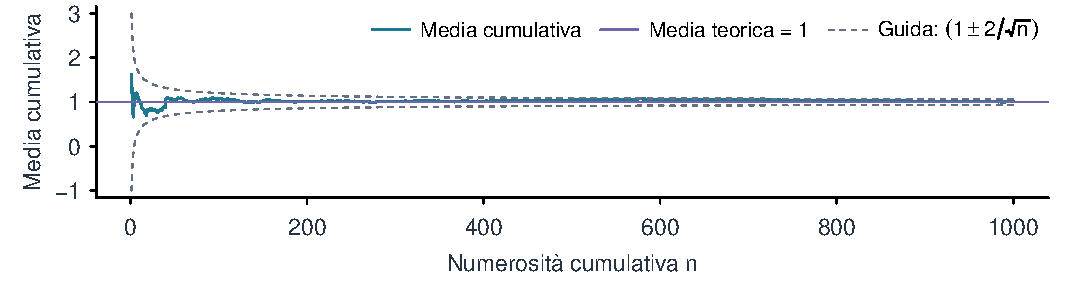
\includegraphics[width=\linewidth]{lln_leggibile.pdf}\par\nointerlineskip
\begin{minipage}[t]{10.05cm}\vspace{0pt}
\PCode{Una media per ogni numerosità cumulativa}{45_media_cumulativa.R}
\end{minipage}\hfill
\begin{minipage}[t]{7.55cm}\vspace{0pt}
\PSmall{Nuova simulazione: $X_i\sim\operatorname{Exp}(1)$ indipendenti, $\mu=\sigma=1$. Le medie sono cumulative.}
\PSmall{Le linee $1\pm2/\sqrt n$ mostrano la scala dell'errore standard. La banda non è un intervallo esatto e non offre copertura simultanea.}
\end{minipage}

\end{minipage}%
\end{lrbox}
\typeout{FULLBOX:045:W:\the\ht\FullWideBox:\the\dp\FullWideBox}
\begin{frame}[plain]\hypertarget{slide45}{}
\bookmark[level=1,page=45]{Convergenza della media campionaria}
\begin{tikzpicture}[remember picture,overlay]
\PilotChrome{Convergenza della media campionaria}{Campionamento e statistica}{45}{Controllare l'andamento della media cumulativa; una fluttuazione locale resta possibile anche per campioni grandi.}
\node[anchor=north west,inner sep=0] at ([xshift=0.96cm,yshift=-2.13cm]current page.north west) {\usebox{\FullWideBox}};
\end{tikzpicture}
\end{frame}

% SLIDE 046 | Teorema del limite centrale | REVISIONE COMPLETA
\begin{lrbox}{\PilotLeftBox}%
\begin{minipage}[t]{10.05cm}\raggedright\color{Ink}\fontsize{11.3}{14.8}\selectfont

\PLabel{Ripetere idealmente il campionamento}
\begin{tikzpicture}[x=1cm,y=1cm]
 \foreach \yy/\lab in {3.5/1,2.3/2,1.1/3}{
  \node[pFlow,text width=3.15cm,minimum height=.75cm] (s\lab) at (2,\yy) {Campione \lab: $n$ valori};
  \node[pFlow,text width=1.6cm,minimum height=.75cm] (m\lab) at (5.2,\yy) {$\bar X^{(\lab)}$};
  \node[pFlow,text width=1.65cm,minimum height=.75cm] (z\lab) at (8.1,\yy) {$Z_n^{(\lab)}$};
  \draw[pEdge] (s\lab.east)--(m\lab.west);
  \draw[pEdge] (m\lab.east)--(z\lab.west);
 }
 \node[pNote] at (5.2,4.35) {Media};
 \node[pNote] at (8.1,4.35) {Standardizzazione};
 \node[pNote] at (4.8,.25) {La distribuzione si costruisce confrontando molte medie.};
\end{tikzpicture}
\[Z_n=\frac{\sqrt n(\bar X_n-\mu)}{\sigma}
 \xrightarrow{\,d\,}\mathcal N(0,1).\]

\end{minipage}%
\end{lrbox}
\typeout{FULLBOX:046:L:\the\ht\PilotLeftBox:\the\dp\PilotLeftBox}
\begin{lrbox}{\PilotRightBox}%
\begin{minipage}[t]{7.55cm}\raggedright\color{Ink}\fontsize{11.3}{14.8}\selectfont

\PLabel{Condizioni e significato}
\PBody{$X_i$ indipendenti e identicamente distribuite, con media $\mu$ e varianza $0<\sigma^2<\infty$.}
\[\mathbb E(\bar X_n)=\mu,\qquad
 \operatorname{Var}(\bar X_n)=\frac{\sigma^2}{n}.\]
\PBody{La standardizzazione centra la media e ne esprime lo scarto in unità di errore standard $\sigma/\sqrt n$.}
\PInfo{La normale approssima la distribuzione delle medie standardizzate. La distribuzione delle singole osservazioni può restare asimmetrica.}

\end{minipage}%
\end{lrbox}
\typeout{FULLBOX:046:R:\the\ht\PilotRightBox:\the\dp\PilotRightBox}
\begin{frame}[plain]\hypertarget{slide46}{}
\bookmark[level=1,page=46]{Teorema del limite centrale}
\begin{tikzpicture}[remember picture,overlay]
\PilotChrome{Teorema del limite centrale}{Campionamento e statistica}{46}{La numerosità necessaria a una buona approssimazione dipende dalla distribuzione di partenza e dalla quantità studiata.}
\node[anchor=north west,inner sep=0] at ([xshift=0.96cm,yshift=-2.13cm]current page.north west) {\usebox{\PilotLeftBox}};
\node[anchor=north west,inner sep=0] at ([xshift=11.52cm,yshift=-2.13cm]current page.north west) {\usebox{\PilotRightBox}};
\end{tikzpicture}
\end{frame}

% SLIDE 047 | Distribuzione delle medie standardizzate | REVISIONE COMPLETA
\begin{lrbox}{\FullWideBox}%
\begin{minipage}[t]{18.1cm}\raggedright\color{Ink}\fontsize{11.3}{14.8}\selectfont

\hspace*{.15cm}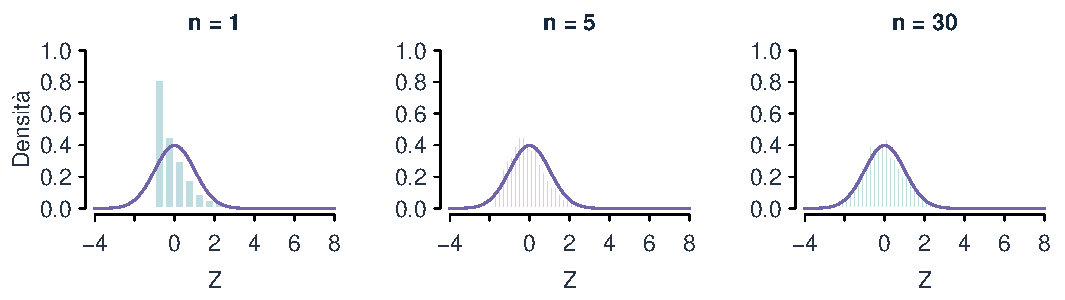
\includegraphics[width=17.8cm]{clt_leggibile.pdf}\par\nointerlineskip
\begin{minipage}[t]{10.05cm}\vspace{0pt}
\PCode{Tre mila medie, ciascuna da un nuovo campione}{47_medie_replicate.R}
\end{minipage}\hfill
\begin{minipage}[t]{7.55cm}\vspace{0pt}
\PSmall{Nuova simulazione da $\operatorname{Exp}(1)$, con $\mu=\sigma=1$. La curva viola è la densità normale standard.}
\PSmall{\texttt{replicate()} estrae ogni volta un nuovo campione. Modificare \texttt{n} in 1, 5 e 30; la qualità dell'approssimazione dipende dalla distribuzione di partenza.}
\end{minipage}

\end{minipage}%
\end{lrbox}
\typeout{FULLBOX:047:W:\the\ht\FullWideBox:\the\dp\FullWideBox}
\begin{frame}[plain]\hypertarget{slide47}{}
\bookmark[level=1,page=47]{Distribuzione delle medie standardizzate}
\begin{tikzpicture}[remember picture,overlay]
\PilotChrome{Distribuzione delle medie standardizzate}{Campionamento e statistica}{47}{Confrontare la distribuzione dei dati grezzi con quella delle medie. Il limite centrale riguarda la seconda, dopo standardizzazione.}
\node[anchor=north west,inner sep=0] at ([xshift=0.96cm,yshift=-2.13cm]current page.north west) {\usebox{\FullWideBox}};
\end{tikzpicture}
\end{frame}

% SLIDE 048 | Campionamento dei ghiacciai alpini | REVISIONE COMPLETA
\begin{lrbox}{\PilotLeftBox}%
\begin{minipage}[t]{10.05cm}\raggedright\color{Ink}\fontsize{11.3}{14.8}\selectfont

\PLabel{Esempio ipotetico: 25 ghiacciai fotografati}
\begin{tikzpicture}[x=1cm,y=1cm]
 \fill[Rule!60] (.25,.5)--(2.2,3.7)--(3.6,1.6)--(5.1,4.15)--(7,1.4)--(8,3.2)--(9.5,.5)--cycle;
 \fill[white] (1.64,2.78)--(2.2,3.7)--(2.8,2.8)--(2.4,2.9)--(2.1,2.63)--cycle;
 \fill[white] (4.46,3.06)--(5.1,4.15)--(5.87,3.03)--(5.45,3.16)--(5.12,2.85)--cycle;
 \fill[white] (7.48,2.26)--(8,3.2)--(8.57,2.17)--(8.18,2.43)--cycle;
 \draw[GeoB,line width=1.5pt,dashed] (.1,.3).. controls (3,.55) and (6,.1)..(9.5,.45);
 \foreach \xx/\yy in {1.7/2.9,2.5/2.9,7.7/2.55}
  \fill[GeoA] (\xx,\yy) circle(.09);
 \draw[GeoC,line width=1pt] (5.1,3.4) circle(.13);
 \node[pNote,anchor=west] at (.4,4.1) {Accessibilità diseguale};
 \node[pNote,anchor=west,text=GeoB] at (.3,-.15) {Percorso di accesso};
\end{tikzpicture}
\PBody{Una documentazione dal 1950 seleziona i siti per cui esistono immagini confrontabili. Valutare quota, esposizione, dimensione e accessibilità dei ghiacciai osservati e non osservati.}

\end{minipage}%
\end{lrbox}
\typeout{FULLBOX:048:L:\the\ht\PilotLeftBox:\the\dp\PilotLeftBox}
\begin{lrbox}{\PilotRightBox}%
\begin{minipage}[t]{7.55cm}\raggedright\color{Ink}\fontsize{11.3}{14.8}\selectfont

\PLabel{Definire la quantità da confrontare}
\[r_i=100\,\frac{A_{i,t_1}-A_{i,t_0}}{A_{i,t_0}}.\]
\PSmall{$A_{i,t}$: area del ghiacciaio $i$ al tempo $t$; $r_i$: variazione percentuale, negativa in caso di riduzione.}
\[\bar r=\frac1G\sum_{i=1}^{G}r_i.\]
\PBody{Questa media attribuisce lo stesso peso ai $G$ ghiacciai. La variazione percentuale dell'area totale usa i pesi delle aree iniziali.}


\end{minipage}%
\end{lrbox}
\typeout{FULLBOX:048:R:\the\ht\PilotRightBox:\the\dp\PilotRightBox}
\begin{frame}[plain]\hypertarget{slide48}{}
\bookmark[level=1,page=48]{Campionamento dei ghiacciai alpini}
\begin{tikzpicture}[remember picture,overlay]
\PilotChrome{Campionamento dei ghiacciai alpini}{Campionamento e statistica}{48}{Specificare se l'obiettivo riguarda il ghiacciaio medio o l'area glaciale complessiva, e quali siti possono essere rappresentati.}
\node[anchor=north west,inner sep=0] at ([xshift=0.96cm,yshift=-2.13cm]current page.north west) {\usebox{\PilotLeftBox}};
\node[anchor=north west,inner sep=0] at ([xshift=11.52cm,yshift=-2.13cm]current page.north west) {\usebox{\PilotRightBox}};
\end{tikzpicture}
\end{frame}

% SLIDE 049 | Campionamento delle coste mediterranee | REVISIONE COMPLETA
\begin{lrbox}{\PilotLeftBox}%
\begin{minipage}[t]{10.05cm}\raggedright\color{Ink}\fontsize{11.3}{14.8}\selectfont

\PLabel{Il mareografo misura un livello relativo}
\begin{tikzpicture}[x=1cm,y=1cm]
 \fill[GeoA!12] (.2,.4) rectangle (6.2,2.4);
 \fill[GeoB!15] (6.2,.4)--(6.2,2)--(7.3,2.65)--(9.4,2.65)--(9.4,.4)--cycle;
 \draw[GeoA,line width=1.2pt] (.2,2.4)--(6.8,2.4);
 \draw[Muted,dashed] (.2,.7)--(9.4,.7);
 \draw[pAxis] (1.1,.7)--(1.1,2.4);
 \node[pNote,anchor=west] at (1.3,1.5) {$h_{\mathrm{mare}}$};
 \draw[pAxis] (8.5,.7)--(8.5,2.65);
 \node[pNote,anchor=east] at (8.2,1.55) {$h_{\mathrm{suolo}}$};
 \draw[Navy,line width=2pt] (6.75,1.6)--(6.75,3.3);
 \node[pNote,anchor=south] at (6.75,3.4) {Mareografo};
 \node[pNote,anchor=west] at (.2,.1) {Riferimento verticale comune, schema illustrativo};
\end{tikzpicture}
\[h_{\mathrm{rel}}=h_{\mathrm{mare}}-h_{\mathrm{suolo}}.\]
\PBody{Una rete ipotetica di 12 mareografi con almeno 30 anni di dati descrive i siti strumentati. Porti, moto verticale del suolo e condizioni locali influiscono sul confronto.}

\end{minipage}%
\end{lrbox}
\typeout{FULLBOX:049:L:\the\ht\PilotLeftBox:\the\dp\PilotLeftBox}
\begin{lrbox}{\PilotRightBox}%
\begin{minipage}[t]{7.55cm}\raggedright\color{Ink}\fontsize{11.3}{14.8}\selectfont

\PCode{Tre tempi in un esempio simulato}{49_livello_relativo.R}
\PSmall{Gli incrementi sono espressi in mm rispetto al tempo iniziale. Se il suolo scende, la variazione del livello relativo aumenta.}
\PInfo{Verificare riferimenti verticali, spostamenti degli strumenti e copertura delle serie. La media dei siti non attribuisce automaticamente lo stesso peso a ogni tratto di costa.}

\end{minipage}%
\end{lrbox}
\typeout{FULLBOX:049:R:\the\ht\PilotRightBox:\the\dp\PilotRightBox}
\begin{frame}[plain]\hypertarget{slide49}{}
\bookmark[level=1,page=49]{Campionamento delle coste mediterranee}
\begin{tikzpicture}[remember picture,overlay]
\PilotChrome{Campionamento delle coste mediterranee}{Campionamento e statistica}{49}{Dichiarare il riferimento verticale e distinguere variazione del mare, movimento del suolo e livello relativo osservato.}
\node[anchor=north west,inner sep=0] at ([xshift=0.96cm,yshift=-2.13cm]current page.north west) {\usebox{\PilotLeftBox}};
\node[anchor=north west,inner sep=0] at ([xshift=11.52cm,yshift=-2.13cm]current page.north west) {\usebox{\PilotRightBox}};
\end{tikzpicture}
\end{frame}

% SLIDE 050 | Permafrost: durata e posizione delle misure | REVISIONE COMPLETA
\begin{lrbox}{\PilotLeftBox}%
\begin{minipage}[t]{10.05cm}\raggedright\color{Ink}\fontsize{11.3}{14.8}\selectfont

\PLabel{Sito, profondità e tempo identificano la misura}
\begin{tikzpicture}[x=1cm,y=.85cm]
 \fill[GeoB!12] (.3,.3) rectangle (9.4,3.15);
 \draw[Muted,line width=.9pt] (.3,3.15)--(9.4,3.15);
 \foreach \xx/\lab in {2.6/Sito 1,7.1/Sito 2}{
  \draw[Navy,line width=1.8pt] (\xx,.55)--(\xx,3.5);
  \foreach \yy in {.8,1.55,2.3}\fill[GeoA] (\xx,\yy) circle(.1);
  \node[pLabel] at (\xx,3.9) {\lab};
 }
 \draw[pAxis] (.8,2.9)--(.8,.6);
 \node[pNote,rotate=90] at (.4,1.75) {Profondità $z$};
 \node[pNote,text width=3.4cm] at (2.6,-.25) {Esposizione e materiale\\da documentare};
 \node[pNote,text width=3.4cm] at (7.1,-.25) {Stesse profondità e tempi\\per confronti coerenti};
\end{tikzpicture}
\[X=X(s,z,t).\]
\PSmall{$s$: posizione; $z$: profondità; $t$: tempo. Nell'esempio: otto fori oltre 2500 m, cinque anni di osservazione.}

\end{minipage}%
\end{lrbox}
\typeout{FULLBOX:050:L:\the\ht\PilotLeftBox:\the\dp\PilotLeftBox}
\begin{lrbox}{\PilotRightBox}%
\begin{minipage}[t]{7.55cm}\raggedright\color{Ink}\fontsize{11.3}{14.8}\selectfont

\PCode{Costruire il piano delle osservazioni}{50_piano_permafrost.R}
\PSmall{\texttt{each=5} ripete ogni sito cinque volte; \texttt{times=8} ripete la sequenza degli anni. La tabella controlla la copertura prevista.}
\PInfo{Quaranta coppie sito--anno descrivono otto siti seguiti nel tempo. Cinque anni possono essere insufficienti a separare una tendenza dalla variabilità interannuale.}

\end{minipage}%
\end{lrbox}
\typeout{FULLBOX:050:R:\the\ht\PilotRightBox:\the\dp\PilotRightBox}
\begin{frame}[plain]\hypertarget{slide50}{}
\bookmark[level=1,page=50]{Permafrost: durata e posizione delle misure}
\begin{tikzpicture}[remember picture,overlay]
\PilotChrome{Permafrost: durata e posizione delle misure}{Campionamento e statistica}{50}{Confrontare misure alla stessa profondità e documentare durata, frequenza, esposizione e distribuzione dei fori.}
\node[anchor=north west,inner sep=0] at ([xshift=0.96cm,yshift=-2.13cm]current page.north west) {\usebox{\PilotLeftBox}};
\node[anchor=north west,inner sep=0] at ([xshift=11.52cm,yshift=-2.13cm]current page.north west) {\usebox{\PilotRightBox}};
\end{tikzpicture}
\end{frame}

% SLIDE 051 | Depositi fluviali e pseudoreplicazione | REVISIONE COMPLETA
\begin{lrbox}{\PilotLeftBox}%
\begin{minipage}[t]{10.05cm}\raggedright\color{Ink}\fontsize{11.3}{14.8}\selectfont

\PLabel{Dieci carote in due unità geomorfologiche}
\begin{tikzpicture}[x=1cm,y=1cm]
 \draw[GeoA!25,line width=17pt] (.2,2)..controls(2.4,3.9)and(4.6,.5)..(6.2,2.1)..controls(7.2,3.4)and(8.2,3.2)..(9.3,2.4);
 \foreach \xx/\col/\lab in {2.4/GeoA/1,7.2/GeoC/2}{
  \draw[pGroup,fill=\col!9] (\xx-1.6,.45) rectangle (\xx+1.6,2.9);
  \foreach \dx/\dy in {-.9/1.25,-.45/.8,0/1.5,.5/.75,.95/1.3}{
   \draw[\col,line width=2pt] (\xx+\dx,\dy)--(\xx+\dx,\dy+.55);
  }
  \node[pNote] at (\xx,2.5) {Unità \lab};
 }
 \node[pNote] at (4.8,3.6) {Le carote della stessa unità condividono una componente.};
\end{tikzpicture}
\PBody{La numerosità delle carote è $n=10$; le unità geomorfologiche rappresentate sono $G=2$. La dipendenza interna deve entrare nel modello e nel disegno.}

\end{minipage}%
\end{lrbox}
\typeout{FULLBOX:051:L:\the\ht\PilotLeftBox:\the\dp\PilotLeftBox}
\begin{lrbox}{\PilotRightBox}%
\begin{minipage}[t]{7.55cm}\raggedright\color{Ink}\fontsize{11.3}{14.8}\selectfont


\[X_{ij}=\mu+u_j+\varepsilon_{ij}.\]
\PSmall{$\mu$: media comune. Gli effetti $u_j$, di varianza $\tau^2$, e gli errori $\varepsilon_{ij}$, di varianza $\sigma^2$, hanno media zero e sono indipendenti. Ogni $u_j$ è condiviso dalle carote dell'unità $j$.}
\[\operatorname{Cov}(X_{ij},X_{kj})=\tau^2
 \quad(i\neq k).\]
\PInfo{Con $m$ carote per unità, la varianza della media è $\tau^2/G+\sigma^2/(Gm)$. Aumentare $m$ riduce soltanto il secondo termine.}
\PSmall{Questo modello introduce dipendenza interna. Terra01 genera invece errori indipendenti attorno a tre medie fissate.}

\end{minipage}%
\end{lrbox}
\typeout{FULLBOX:051:R:\the\ht\PilotRightBox:\the\dp\PilotRightBox}
\begin{frame}[plain]\hypertarget{slide51}{}
\bookmark[level=1,page=51]{Depositi fluviali e pseudoreplicazione}
\begin{tikzpicture}[remember picture,overlay]
\PilotChrome{Depositi fluviali e pseudoreplicazione}{Campionamento e statistica}{51}{Distinguere campioni raccolti, siti e unità geomorfologiche. Repliche ravvicinate possono condividere la stessa informazione.}
\node[anchor=north west,inner sep=0] at ([xshift=0.96cm,yshift=-2.13cm]current page.north west) {\usebox{\PilotLeftBox}};
\node[anchor=north west,inner sep=0] at ([xshift=11.52cm,yshift=-2.13cm]current page.north west) {\usebox{\PilotRightBox}};
\end{tikzpicture}
\end{frame}

% SLIDE 052 | Moda ed effetto di un valore estremo | REVISIONE COMPLETA
\begin{lrbox}{\PilotLeftBox}%
\begin{minipage}[t]{10.05cm}\raggedright\color{Ink}\fontsize{11.3}{14.8}\selectfont

\PLabel{I valori 3, 4, 5 e 100}
\begin{tikzpicture}[x=.085cm,y=1cm]
 \draw[pAxis] (0,.8)--(108,.8);
 \foreach \xx in {0,25,50,75,100}{
  \draw[Muted] (\xx,.72)--(\xx,.88);
  \node[pNote,below] at (\xx,.65) {\xx};
 }
 \foreach \xx/\yy in {3/1.1,4/1.4,5/1.7,100/1.1}
  \fill[GeoA] (\xx,\yy) circle[x radius=1,y radius=.085];
 \draw[GeoB,line width=1.1pt] (28,.8)--(28,2.8);
 \node[pNote,text=GeoB] at (28,3.1) {Media: 28};
 \draw[GeoC,line width=1pt] (4.5,.8)--(4.5,2.2)--(10,2.6);
 \node[pNote,text=GeoC,anchor=west] at (10,2.6) {Mediana: 4.5};
\end{tikzpicture}
\[\bar x=\frac{3+4+5+100}{4}=28,\qquad
 \tilde x=\frac{4+5}{2}=4.5.\]
\PBody{La media incorpora l'entità di ogni valore. La mediana usa le posizioni nell'ordinamento ed è meno sensibile a un singolo valore molto distante.}

\end{minipage}%
\end{lrbox}
\typeout{FULLBOX:052:L:\the\ht\PilotLeftBox:\the\dp\PilotLeftBox}
\begin{lrbox}{\PilotRightBox}%
\begin{minipage}[t]{7.55cm}\raggedright\color{Ink}\fontsize{11.3}{14.8}\selectfont

\PCode{Calcolare e contare}{52_posizione.R}
\PSmall{I quattro valori hanno frequenza uno. Nessuno è più frequente degli altri: una moda unica non è definita per questo campione.}
\PInfo{In R, \texttt{mode()} indica la modalità di memorizzazione dell'oggetto. Per la moda statistica si esaminano le frequenze con \texttt{table()}.}

\end{minipage}%
\end{lrbox}
\typeout{FULLBOX:052:R:\the\ht\PilotRightBox:\the\dp\PilotRightBox}
\begin{frame}[plain]\hypertarget{slide52}{}
\bookmark[level=1,page=52]{Moda ed effetto di un valore estremo}
\begin{tikzpicture}[remember picture,overlay]
\PilotChrome{Moda ed effetto di un valore estremo}{Campionamento e statistica}{52}{La sensibilità della media a valori elevati fa parte della sua definizione. Verificare l'osservazione prima di decidere come trattarla.}
\node[anchor=north west,inner sep=0] at ([xshift=0.96cm,yshift=-2.13cm]current page.north west) {\usebox{\PilotLeftBox}};
\node[anchor=north west,inner sep=0] at ([xshift=11.52cm,yshift=-2.13cm]current page.north west) {\usebox{\PilotRightBox}};
\end{tikzpicture}
\end{frame}

% SLIDE 053 | Indicatori di posizione nei dati ambientali | REVISIONE COMPLETA
\begin{lrbox}{\PilotLeftBox}%
\begin{minipage}[t]{10.05cm}\raggedright\color{Ink}\fontsize{11.3}{14.8}\selectfont

\PLabel{L'indicatore dipende dalla scala di misura}
\begin{tikzpicture}[x=1cm,y=1cm]
 \node[pFlow,text width=3.9cm,minimum height=1.05cm] (a) at (2.2,3.6) {Temperatura $[^\circ\mathrm C]$\\variabile quantitativa};
 \node[pFlow,text width=3.9cm,minimum height=1.05cm] (b) at (2.2,1.95) {Precipitazione [mm]\\possibile coda destra};
 \node[pFlow,text width=3.9cm,minimum height=1.05cm] (c) at (2.2,.3) {Tipo di sedimento\\categoria nominale};
 \node[pLabel,text width=3.7cm] (ar) at (7.1,3.6) {Media, mediana\\e dispersione};
 \node[pLabel,text width=3.7cm] (br) at (7.1,1.95) {Media, mediana, quantili\\e frequenza di pioggia};
 \node[pLabel,text width=3.7cm] (cr) at (7.1,.3) {Frequenze\\e categoria modale};
 \draw[pEdge] (a.east)--(ar.west);
 \draw[pEdge] (b.east)--(br.west);
 \draw[pEdge] (c.east)--(cr.west);
\end{tikzpicture}
\PBody{Attribuire numeri alle categorie non rende significativa la loro media. Nei dati quantitativi, affiancare alla sintesi un controllo di forma, unità e possibili errori di trascrizione.}

\end{minipage}%
\end{lrbox}
\typeout{FULLBOX:053:L:\the\ht\PilotLeftBox:\the\dp\PilotLeftBox}
\begin{lrbox}{\PilotRightBox}%
\begin{minipage}[t]{7.55cm}\raggedright\color{Ink}\fontsize{11.3}{14.8}\selectfont

\PCode{Individuare le categorie più frequenti}{53_moda.R}
\PSmall{\texttt{table()} conta le occorrenze. Il confronto con la frequenza massima conserva tutte le categorie in caso di parità.}
\[\mathcal M=\{c:f_c=\max_k f_k\}.\]
\PSmall{$f_c$: frequenza della categoria $c$; $\mathcal M$: insieme delle categorie modali. Nell'esempio contiene \texttt{sabbia}.}

\end{minipage}%
\end{lrbox}
\typeout{FULLBOX:053:R:\the\ht\PilotRightBox:\the\dp\PilotRightBox}
\begin{frame}[plain]\hypertarget{slide53}{}
\bookmark[level=1,page=53]{Indicatori di posizione nei dati ambientali}
\begin{tikzpicture}[remember picture,overlay]
\PilotChrome{Indicatori di posizione nei dati ambientali}{Campionamento e statistica}{53}{Scegliere indicatori compatibili con la variabile, l'unità di misura e la domanda scientifica.}
\node[anchor=north west,inner sep=0] at ([xshift=0.96cm,yshift=-2.13cm]current page.north west) {\usebox{\PilotLeftBox}};
\node[anchor=north west,inner sep=0] at ([xshift=11.52cm,yshift=-2.13cm]current page.north west) {\usebox{\PilotRightBox}};
\end{tikzpicture}
\end{frame}

% SLIDE 054 | Dispersione: ampiezza, deviazione standard, IQR | REVISIONE COMPLETA
\begin{lrbox}{\PilotLeftBox}%
\begin{minipage}[t]{10.05cm}\raggedright\color{Ink}\fontsize{11.3}{14.8}\selectfont

\PLabel{Quale distanza si vuole riassumere?}
\begin{tikzpicture}[x=1cm,y=1cm]
\draw[pAxis] (0,.7)--(8.1,.7) node[right,pNote]{mg/L};
\foreach \xx in {1,...,7}{\draw[Muted](\xx,.65)--(\xx,.75);\node[pNote,below] at (\xx,.6){\xx};}
\foreach \xx/\yy in {1/1.05,2/1.05,2/1.30,3/1.05,7/1.05}{\fill[GeoA](\xx,\yy)circle(2pt);}
\draw[Classical,line width=3pt](2,1.85)--(3,1.85);
\draw[Classical](2,1.65)--(2,2.05) (3,1.65)--(3,2.05);
\node[pNote,above] at (2.5,2.1){IQR = 1};
\draw[GeoB,{Latex[length=1.8mm]}-{Latex[length=1.8mm]}](1,2.8)--(7,2.8);
\node[pNote,above] at (4,2.8){ampiezza = 7 $-$ 1 = 6};
\end{tikzpicture}
\[s=\sqrt{\frac{\sum_{i=1}^{n}(x_i-\bar x)^2}{n-1}},\qquad \mathrm{IQR}=Q_3-Q_1\]
\PBody{$s$ misura gli scarti dalla media; l'IQR descrive la metà centrale delle osservazioni. Entrambi hanno l'unità di $x$.}

\end{minipage}%
\end{lrbox}
\typeout{FULLBOX:054:L:\the\ht\PilotLeftBox:\the\dp\PilotLeftBox}
\begin{lrbox}{\PilotRightBox}%
\begin{minipage}[t]{7.55cm}\raggedright\color{Ink}\fontsize{11.3}{14.8}\selectfont

\PCode{R · tre misure di dispersione}{54_dispersione.R}
\PInfo{$n$ è il numero di misure, $Q_1$ e $Q_3$ sono i quartili. In R, \texttt{sd()} usa il divisore $n-1$; \texttt{quantile()} usa di default l'interpolazione di tipo 7.}
\PSmall{L'ampiezza dipende solo dai due estremi. La deviazione standard usa tutte le distanze dalla media.}

\end{minipage}%
\end{lrbox}
\typeout{FULLBOX:054:R:\the\ht\PilotRightBox:\the\dp\PilotRightBox}
\begin{frame}[plain]\hypertarget{slide54}{}
\bookmark[level=1,page=54]{Dispersione: ampiezza, deviazione standard, IQR}
\begin{tikzpicture}[remember picture,overlay]
\PilotChrome{Dispersione: ampiezza, deviazione standard, IQR}{STATISTICA DESCRITTIVA}{54}{Indicare sempre quale misura di dispersione si usa; ampiezza, deviazione standard e IQR descrivono aspetti diversi.}
\node[anchor=north west,inner sep=0] at ([xshift=0.96cm,yshift=-2.13cm]current page.north west) {\usebox{\PilotLeftBox}};
\node[anchor=north west,inner sep=0] at ([xshift=11.52cm,yshift=-2.13cm]current page.north west) {\usebox{\PilotRightBox}};
\end{tikzpicture}
\end{frame}

% SLIDE 055 | Posizione e dispersione cambiano separatamente | REVISIONE COMPLETA
\begin{lrbox}{\PilotLeftBox}%
\begin{minipage}[t]{10.05cm}\raggedright\color{Ink}\fontsize{11.3}{14.8}\selectfont

\PLabel{Tre serie schematiche sulla stessa scala}
\begin{tikzpicture}[x=.72cm,y=1cm]
\foreach \yy/\lab in {3/A,2/B,1/C}{\draw[Rule](0,\yy)--(12,\yy);\node[pLabel,left]at(0,\yy){\lab};}
\foreach \xx in {2,3,4,5,6}{\fill[GeoA](\xx,3)circle(2.4pt);}
\foreach \xx in {7,8,9,10,11}{\fill[GeoB](\xx,2)circle(2.4pt);}
\foreach \xx in {0,2,4,6,8}{\fill[GeoC](\xx,1)circle(2.4pt);}
\foreach \xx/\lab in {0/{$-1$},2/1,4/3,6/5,8/7,10/9}{\node[pNote,below]at(\xx,.6){\lab};}
\node[pNote,anchor=west]at(.2,3.75){A e B: stessa forma, medie diverse};
\node[pNote,anchor=west]at(.2,.05){A e C: stessa media, dispersioni diverse};
\end{tikzpicture}
\[\overline{x+a}=\bar x+a,\qquad s_{x+a}=s_x,\qquad s_{b x}=|b|s_x\]
\PSmall{$a$ è uno spostamento costante, $b$ un fattore di scala. Nelle serie ambientali confrontare anche stagione e frequenza delle misure.}

\end{minipage}%
\end{lrbox}
\typeout{FULLBOX:055:L:\the\ht\PilotLeftBox:\the\dp\PilotLeftBox}
\begin{lrbox}{\PilotRightBox}%
\begin{minipage}[t]{7.55cm}\raggedright\color{Ink}\fontsize{11.3}{14.8}\selectfont
\PCode{R · spostare e dilatare i dati}{55_posizione_dispersione.R}
\PSmall{Una mareggiata può modificare gli estremi e la dispersione senza descrivere l'oscillazione abituale del livello marino.}
\PSmall{Confrontare periodi con uguale durata e frequenza delle misure. Anche la stagionalità può aumentare $s$.}
\end{minipage}%
\end{lrbox}
\typeout{FULLBOX:055:R:\the\ht\PilotRightBox:\the\dp\PilotRightBox}
\begin{frame}[plain]\hypertarget{slide55}{}
\bookmark[level=1,page=55]{Posizione e dispersione cambiano separatamente}
\begin{tikzpicture}[remember picture,overlay]
\PilotChrome{Posizione e dispersione cambiano separatamente}{STATISTICA DESCRITTIVA}{55}{Una media maggiore non implica una dispersione maggiore. Per confrontare due serie servono entrambe le informazioni.}
\node[anchor=north west,inner sep=0] at ([xshift=0.96cm,yshift=-2.13cm]current page.north west) {\usebox{\PilotLeftBox}};
\node[anchor=north west,inner sep=0] at ([xshift=11.52cm,yshift=-2.13cm]current page.north west) {\usebox{\PilotRightBox}};
\end{tikzpicture}
\end{frame}

% SLIDE 056 | Precipitazione giornaliera: media e mediana | REVISIONE COMPLETA
\begin{lrbox}{\PilotLeftBox}%
\begin{minipage}[t]{10.05cm}\raggedright\color{Ink}\fontsize{11.3}{14.8}\selectfont

\PLabel{Roma/Ciampino · 2024 · 361 giorni con dati}
\begin{center}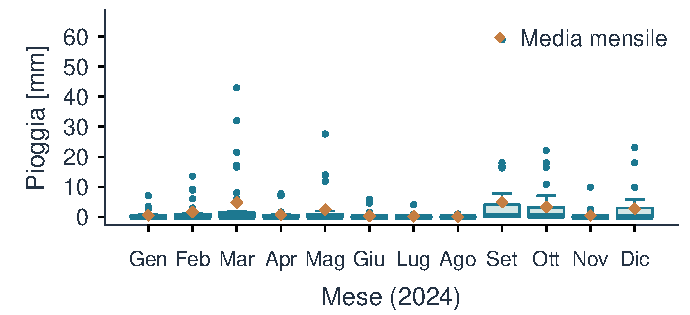
\includegraphics[width=\linewidth,height=4.8cm,keepaspectratio]{plot_median_media.pdf}\end{center}
\PSmall{La linea nel box è la mediana; il rombo indica la media. Giorni asciutti ed eventi intensi producono asimmetria. Fonte: Meteostat, incluse stime di modello.}

\end{minipage}%
\end{lrbox}
\typeout{FULLBOX:056:L:\the\ht\PilotLeftBox:\the\dp\PilotLeftBox}
\begin{lrbox}{\PilotRightBox}%
\begin{minipage}[t]{7.55cm}\raggedright\color{Ink}\fontsize{11.3}{14.8}\selectfont
\PCode{Prova su dati simulati}{56_media_mediana_mese.R}
\PSmall{\texttt{tapply()} applica la stessa funzione a ciascun mese.}
\[\bar p=\frac{n_+}{n}\,\bar p_+\]
\PSmall{$n_+$ conta i giorni piovosi; $\bar p_+$ è la media su quei giorni. La media giornaliera dipende da frequenza e intensità degli eventi.}
\end{minipage}%
\end{lrbox}
\typeout{FULLBOX:056:R:\the\ht\PilotRightBox:\the\dp\PilotRightBox}
\begin{frame}[plain]\hypertarget{slide56}{}
\bookmark[level=1,page=56]{Precipitazione giornaliera: media e mediana}
\begin{tikzpicture}[remember picture,overlay]
\PilotChrome{Precipitazione giornaliera: media e mediana}{STATISTICA DESCRITTIVA}{56}{Con molti giorni senza pioggia, la mediana può essere zero anche quando la precipitazione media è positiva.}
\node[anchor=north west,inner sep=0] at ([xshift=0.96cm,yshift=-2.13cm]current page.north west) {\usebox{\PilotLeftBox}};
\node[anchor=north west,inner sep=0] at ([xshift=11.52cm,yshift=-2.13cm]current page.north west) {\usebox{\PilotRightBox}};
\end{tikzpicture}
\end{frame}

% SLIDE 057 | Correlazione lineare: segno e intensità | REVISIONE COMPLETA
\begin{lrbox}{\PilotLeftBox}%
\begin{minipage}[t]{10.05cm}\raggedright\color{Ink}\fontsize{11.3}{14.8}\selectfont

\PLabel{Il coefficiente riassume l'allineamento}
\begin{tikzpicture}[x=1cm,y=1cm]
\foreach \off/\lab in {0/{$r=1$},3.2/{$r=-1$},6.4/{$r=0$}}{
\begin{scope}[xshift=\off cm]\draw[pAxis](0,0)--(2.4,0);\draw[pAxis](0,0)--(0,2.3);\node[pNote]at(1.1,2.65){\lab};\end{scope}}
\foreach \xx/\yy in {.3/.3,.7/.7,1.1/1.1,1.5/1.5,1.9/1.9}{\fill[GeoA](\xx,\yy)circle(2pt);}
\foreach \xx/\yy in {.3/1.9,.7/1.5,1.1/1.1,1.5/.7,1.9/.3}{\fill[GeoB]({\xx+3.2},\yy)circle(2pt);}
\foreach \xx/\yy in {.3/1.9,.7/.7,1.1/.3,1.5/.7,1.9/1.9}{\fill[GeoC]({\xx+6.4},\yy)circle(2pt);}
\end{tikzpicture}
\[r=\frac{\sum_i(x_i-\bar x)(y_i-\bar y)}{\sqrt{\sum_i(x_i-\bar x)^2\sum_i(y_i-\bar y)^2}}\]
\PSmall{Ogni punto è una coppia $(x_i,y_i)$. Occorrono dispersioni non nulle. $-1\leq r\leq1$; $r$ non ha unità. La relazione curva a destra ha $r=0$.}

\end{minipage}%
\end{lrbox}
\typeout{FULLBOX:057:L:\the\ht\PilotLeftBox:\the\dp\PilotLeftBox}
\begin{lrbox}{\PilotRightBox}%
\begin{minipage}[t]{7.55cm}\raggedright\color{Ink}\fontsize{11.3}{14.8}\selectfont
\PCode{R · correlazione e grafico}{57_correlazione.R}
\PSmall{\texttt{complete.cases()} identifica le righe complete. Riportare il numero di coppie insieme al coefficiente.}
\PSmall{In \texttt{demo}, dati simulati, due variabili condividono una stagione. Un'associazione può dipendere da cause comuni.}
\end{minipage}%
\end{lrbox}
\typeout{FULLBOX:057:R:\the\ht\PilotRightBox:\the\dp\PilotRightBox}
\begin{frame}[plain]\hypertarget{slide57}{}
\bookmark[level=1,page=57]{Correlazione lineare: segno e intensità}
\begin{tikzpicture}[remember picture,overlay]
\PilotChrome{Correlazione lineare: segno e intensità}{STATISTICA DESCRITTIVA}{57}{Interpretare r insieme al diagramma a dispersione, al numero di coppie e al processo che ha prodotto i dati.}
\node[anchor=north west,inner sep=0] at ([xshift=0.96cm,yshift=-2.13cm]current page.north west) {\usebox{\PilotLeftBox}};
\node[anchor=north west,inner sep=0] at ([xshift=11.52cm,yshift=-2.13cm]current page.north west) {\usebox{\PilotRightBox}};
\end{tikzpicture}
\end{frame}

% SLIDE 058 | Due associazioni nei dati meteorologici del 2024 | REVISIONE COMPLETA
\begin{lrbox}{\FullWideBox}%
\begin{minipage}[t]{18.1cm}\raggedright\color{Ink}\fontsize{11.3}{14.8}\selectfont

\begin{minipage}[t]{8.8cm}
\PLabel{Sole e temperatura massima}
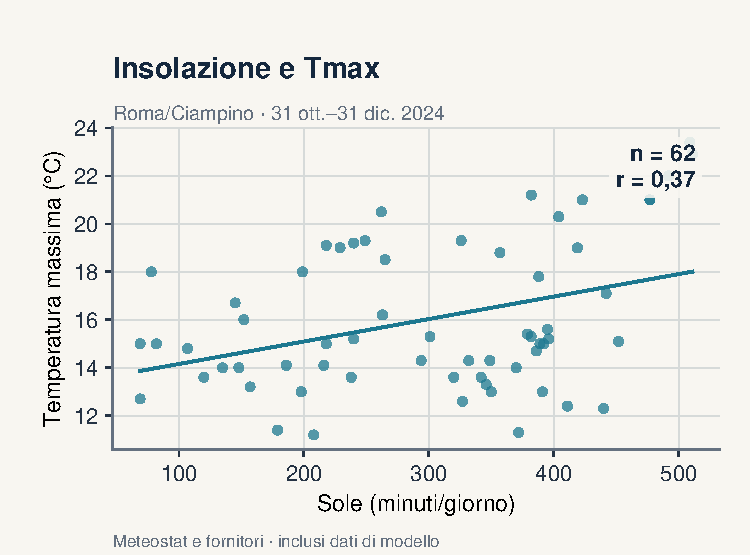
\includegraphics[width=\linewidth,height=5.0cm,keepaspectratio]{cor_pos_2024.pdf}
\PBody{$r\simeq0{,}37$: associazione lineare positiva nel campione di coppie disponibili.}
\end{minipage}\hfill
\begin{minipage}[t]{8.8cm}
\PLabel{Sole e nuvolosità}
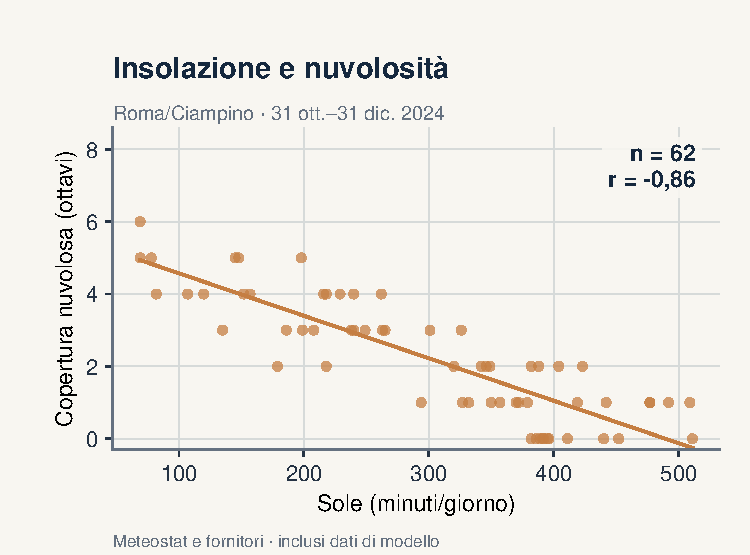
\includegraphics[width=\linewidth,height=5.0cm,keepaspectratio]{cor_neg_2024.pdf}
\PBody{$r\simeq-0{,}86$: associazione lineare negativa. Nuvolosità espressa in ottavi.}
\end{minipage}
\vspace{2mm}
\PSmall{Roma/Ciampino, Meteostat; incluse stime di modello. Entrambe le relazioni usano $n=62$ coppie complete, dal 31 ottobre al 31 dicembre 2024. Il sole è in minuti al giorno. Il periodo copre solo la parte finale dell'anno.}

\end{minipage}%
\end{lrbox}
\typeout{FULLBOX:058:W:\the\ht\FullWideBox:\the\dp\FullWideBox}
\begin{frame}[plain]\hypertarget{slide58}{}
\bookmark[level=1,page=58]{Due associazioni nei dati meteorologici del 2024}
\begin{tikzpicture}[remember picture,overlay]
\PilotChrome{Due associazioni nei dati meteorologici del 2024}{STATISTICA DESCRITTIVA}{58}{Il segno di r riguarda l’associazione nel campione; il risultato può risentire di stagionalità, dati mancanti e cause comuni.}
\node[anchor=north west,inner sep=0] at ([xshift=0.96cm,yshift=-2.13cm]current page.north west) {\usebox{\FullWideBox}};
\end{tikzpicture}
\end{frame}

% SLIDE 059 | Leggere la forma della relazione insieme a r | REVISIONE COMPLETA
\begin{lrbox}{\PilotLeftBox}%
\begin{minipage}[t]{10.05cm}\raggedright\color{Ink}\fontsize{11.3}{14.8}\selectfont

\PLabel{Relazione curva e punto influente}
\begin{tikzpicture}[x=.95cm,y=1cm]
\draw[pAxis](0,0)--(8.6,0) node[right,pNote]{$x$};
\draw[pAxis](0,0)--(0,3.7) node[above,pNote]{$y$};
\draw[Classical,line width=1pt,domain=.7:7.7,samples=50]plot(\x,{.2+.22*(\x-4.2)^2});
\foreach \xx/\yy in {1.2/2.18,2.2/1.08,3.2/.42,4.2/.2,5.2/.42,6.2/1.08,7.2/2.18}{\fill[GeoA](\xx,\yy)circle(2.4pt);}
\draw[GeoB,line width=1pt](1.2,2.18)circle(4pt);
\node[pNote,anchor=west,text width=3cm]at(1.5,3.3){Togliere un estremo rompe la simmetria};
\end{tikzpicture}
\PBody{Per $x=-3,\ldots,3$ e $y=x^2$, $r=0$: gli scarti positivi e negativi si compensano. La dipendenza è evidente nel grafico.}

\end{minipage}%
\end{lrbox}
\typeout{FULLBOX:059:L:\the\ht\PilotLeftBox:\the\dp\PilotLeftBox}
\begin{lrbox}{\PilotRightBox}%
\begin{minipage}[t]{7.55cm}\raggedright\color{Ink}\fontsize{11.3}{14.8}\selectfont
\PCode{R · controllare il disegno dei punti}{59_relazione_curva.R}
\PSmall{\texttt{x[-1]} esclude il primo elemento: qui serve a studiare la sensibilità, senza giustificare esclusioni arbitrarie.}
\PSmall{Riportare la sensibilità al singolo punto insieme alla ragione di un'eventuale esclusione.}
\end{minipage}%
\end{lrbox}
\typeout{FULLBOX:059:R:\the\ht\PilotRightBox:\the\dp\PilotRightBox}
\begin{frame}[plain]\hypertarget{slide59}{}
\bookmark[level=1,page=59]{Leggere la forma della relazione insieme a r}
\begin{tikzpicture}[remember picture,overlay]
\PilotChrome{Leggere la forma della relazione insieme a r}{STATISTICA DESCRITTIVA}{59}{Esaminare forma della relazione, valori influenti e variabili comuni prima di dare un significato scientifico a r.}
\node[anchor=north west,inner sep=0] at ([xshift=0.96cm,yshift=-2.13cm]current page.north west) {\usebox{\PilotLeftBox}};
\node[anchor=north west,inner sep=0] at ([xshift=11.52cm,yshift=-2.13cm]current page.north west) {\usebox{\PilotRightBox}};
\end{tikzpicture}
\end{frame}

% SLIDE 060 | Regressione lineare: retta stimata e residui | REVISIONE COMPLETA
\begin{lrbox}{\PilotLeftBox}%
\begin{minipage}[t]{10.05cm}\raggedright\color{Ink}\fontsize{11.3}{14.8}\selectfont

\[Y_i=\beta_0+\beta_1X_i+\varepsilon_i,\qquad E(\varepsilon_i\mid X_i)=0\]
\begin{tikzpicture}[x=1cm,y=1cm]
\draw[pAxis](0,0)--(8.7,0) node[right,pNote]{$X$};
\draw[pAxis](0,0)--(0,3.7) node[above,pNote]{$Y$};
\draw[Classical,line width=1.3pt](.4,.6)--(8.1,3.0);
\foreach \xx/\yy in {1/.8,2/1.5,3/1.2,4/2.65,5/2.1,6/2.5,7/3.25}{\fill[GeoA](\xx,\yy)circle(2.3pt);}
\draw[GeoB,line width=1pt](4,1.72)--(4,2.65);
\node[pNote,anchor=east,text=GeoB]at(3.85,2.3){$e_i=y_i-\widehat y_i$};
\draw[Muted,dashed](4,1.72)--(6,1.72)--(6,2.35);
\node[pNote,below]at(5,1.72){$\Delta X$};
\node[pNote,right]at(6,2.02){$\widehat\beta_1\Delta X$};
\end{tikzpicture}
\PSmall{$\beta_0$ è l'intercetta, $\beta_1$ la pendenza, $\varepsilon_i$ l'errore del modello. La stima minimizza $\sum_i e_i^2$. Le unità di $\beta_1$ sono quelle di $Y/X$.}

\end{minipage}%
\end{lrbox}
\typeout{FULLBOX:060:L:\the\ht\PilotLeftBox:\the\dp\PilotLeftBox}
\begin{lrbox}{\PilotRightBox}%
\begin{minipage}[t]{7.55cm}\raggedright\color{Ink}\fontsize{11.3}{14.8}\selectfont
\PCode{R · stimare una retta}{60_regressione.R}
\PSmall{In \texttt{tmax \textasciitilde{} tmin}, la risposta precede \texttt{\textasciitilde{}}; la variabile esplicativa segue. \texttt{lm()} restituisce il modello stimato.}
\PSmall{Le temperature di \texttt{demo} sono simulate. La retta descrive un'associazione, senza stabilire da sola una causa.}
\end{minipage}%
\end{lrbox}
\typeout{FULLBOX:060:R:\the\ht\PilotRightBox:\the\dp\PilotRightBox}
\begin{frame}[plain]\hypertarget{slide60}{}
\bookmark[level=1,page=60]{Regressione lineare: retta stimata e residui}
\begin{tikzpicture}[remember picture,overlay]
\PilotChrome{Regressione lineare: retta stimata e residui}{STATISTICA DESCRITTIVA}{60}{La pendenza quantifica una variazione media della risposta per unità di X, nel dominio e nelle condizioni del modello.}
\node[anchor=north west,inner sep=0] at ([xshift=0.96cm,yshift=-2.13cm]current page.north west) {\usebox{\PilotLeftBox}};
\node[anchor=north west,inner sep=0] at ([xshift=11.52cm,yshift=-2.13cm]current page.north west) {\usebox{\PilotRightBox}};
\end{tikzpicture}
\end{frame}

% SLIDE 061 | Prima di interpretare la retta: leggere i residui | REVISIONE COMPLETA
\begin{lrbox}{\PilotLeftBox}%
\begin{minipage}[t]{10.05cm}\raggedright\color{Ink}\fontsize{11.3}{14.8}\selectfont

\PLabel{Tre strutture da riconoscere · schemi}
\begin{tikzpicture}[x=1cm,y=1cm]
\foreach \off/\lab in {0/curvatura,3.2/dispersione,6.4/dipendenza}{
\begin{scope}[xshift=\off cm]\draw[pAxis](0,.3)--(2.5,.3);\draw[Rule](0,1.45)--(2.4,1.45);\node[pNote]at(1.15,3.0){\lab};\end{scope}}
\draw[GeoA,line width=1.1pt,domain=.1:2.3,samples=30]plot(\x,{.5+1.2*(\x-1.2)^2});
\foreach \xx/\yy in {.2/1.4,.4/1.55,.6/1.2,.9/1.8,1.2/.9,1.5/2.2,1.8/.55,2.1/2.6}{\fill[GeoB]({\xx+3.2},\yy)circle(2pt);}
\draw[GeoC,line width=1.1pt]plot[smooth]coordinates{(6.5,1.5)(6.8,2.4)(7.1,2.4)(7.4,1.6)(7.7,.6)(8,.55)(8.3,1.2)(8.6,2.1)};
\node[pNote,below]at(1.1,.15){valori stimati};\node[pNote,below]at(4.3,.15){valori stimati};\node[pNote,below]at(7.5,.15){tempo};
\end{tikzpicture}
\PBody{Curvatura, varianza non costante e dipendenza fra errori possono rendere inadeguate le stime d'incertezza usuali. Controllare anche i punti influenti.}

\end{minipage}%
\end{lrbox}
\typeout{FULLBOX:061:L:\the\ht\PilotLeftBox:\the\dp\PilotLeftBox}
\begin{lrbox}{\PilotRightBox}%
\begin{minipage}[t]{7.55cm}\raggedright\color{Ink}\fontsize{11.3}{14.8}\selectfont
\PCode{R · due controlli complementari}{61_residui.R}
\PSmall{\texttt{fitted()} estrae i valori stimati. \texttt{acf()} confronta la serie con copie ritardate: servono ordine e griglia temporale coerenti.}
\PSmall{Un alto $R^2$ non certifica le ipotesi sugli errori.}
\end{minipage}%
\end{lrbox}
\typeout{FULLBOX:061:R:\the\ht\PilotRightBox:\the\dp\PilotRightBox}
\begin{frame}[plain]\hypertarget{slide61}{}
\bookmark[level=1,page=61]{Prima di interpretare la retta: leggere i residui}
\begin{tikzpicture}[remember picture,overlay]
\PilotChrome{Prima di interpretare la retta: leggere i residui}{STATISTICA DESCRITTIVA}{61}{Per gli intervalli usuali del modello lineare occorre valutare forma della media, varianza e dipendenza degli errori.}
\node[anchor=north west,inner sep=0] at ([xshift=0.96cm,yshift=-2.13cm]current page.north west) {\usebox{\PilotLeftBox}};
\node[anchor=north west,inner sep=0] at ([xshift=11.52cm,yshift=-2.13cm]current page.north west) {\usebox{\PilotRightBox}};
\end{tikzpicture}
\end{frame}

% SLIDE 062 | Intervallo per la media e per una nuova osservazione | REVISIONE COMPLETA
\begin{lrbox}{\PilotLeftBox}%
\begin{minipage}[t]{10.05cm}\raggedright\color{Ink}\fontsize{11.3}{14.8}\selectfont

\PLabel{Roma/Ciampino · 2024 · 366 coppie}
\begin{center}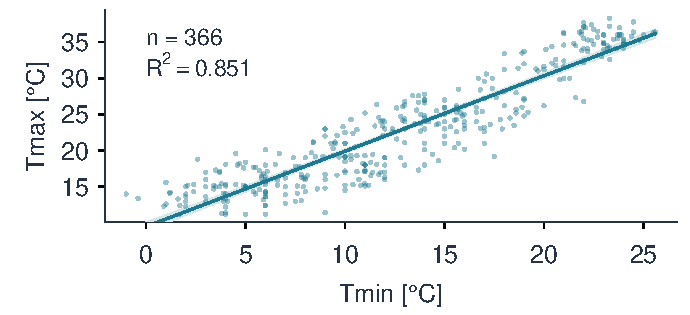
\includegraphics[width=\linewidth,height=4.8cm,keepaspectratio]{regressione_tmax_tmin_2024.pdf}\end{center}
\PSmall{$\widehat T_{\max}=9{,}48+1{,}04T_{\min}$; $R^2=0{,}85$. La fascia rappresenta l'intervallo del 95\% per la media secondo il modello. Fonte: Meteostat, incluse stime di modello.}

\end{minipage}%
\end{lrbox}
\typeout{FULLBOX:062:L:\the\ht\PilotLeftBox:\the\dp\PilotLeftBox}
\begin{lrbox}{\PilotRightBox}%
\begin{minipage}[t]{7.55cm}\raggedright\color{Ink}\fontsize{11.3}{14.8}\selectfont
\PCode{Prova su dati simulati}{62_intervalli_retta.R}
\PSmall{\texttt{confidence} riguarda la media; \texttt{prediction} una nuova osservazione e la dispersione attorno alla retta.}
\PSmall{Entrambi dipendono dalle ipotesi del modello. Nei dati giornalieri verificare stagionalità e autocorrelazione.}
\end{minipage}%
\end{lrbox}
\typeout{FULLBOX:062:R:\the\ht\PilotRightBox:\the\dp\PilotRightBox}
\begin{frame}[plain]\hypertarget{slide62}{}
\bookmark[level=1,page=62]{Intervallo per la media e per una nuova osservazione}
\begin{tikzpicture}[remember picture,overlay]
\PilotChrome{Intervallo per la media e per una nuova osservazione}{STATISTICA DESCRITTIVA}{62}{L’intervallo di previsione di una singola osservazione è più ampio di quello della media, a parità di modello e livello.}
\node[anchor=north west,inner sep=0] at ([xshift=0.96cm,yshift=-2.13cm]current page.north west) {\usebox{\PilotLeftBox}};
\node[anchor=north west,inner sep=0] at ([xshift=11.52cm,yshift=-2.13cm]current page.north west) {\usebox{\PilotRightBox}};
\end{tikzpicture}
\end{frame}

% SLIDE 063 | Importare un CSV: dal testo alle variabili | REVISIONE COMPLETA
\begin{lrbox}{\PilotLeftBox}%
\begin{minipage}[t]{10.05cm}\raggedright\color{Ink}\fontsize{11.3}{14.8}\selectfont

\PLabel{Il tipo di ciascuna colonna va verificato}
\begin{tikzpicture}[x=1cm,y=1cm]
\node[pFlow,text width=8.4cm,minimum height=1.15cm] (csv)at(4.5,4.5){\texttt{data,tmax}\par\texttt{2024-01-01,10.2}};
\node[pFlow,text width=3.7cm,minimum height=1.2cm] (dat)at(2.1,2.3){\texttt{data}\par data del calendario};
\node[pFlow,text width=3.7cm,minimum height=1.2cm] (num)at(6.9,2.3){\texttt{tmax}\par valore numerico};
\draw[pEdge](csv.south)--(4.5,3.45)-|(dat.north);
\draw[pEdge](4.5,3.45)-|(num.north);
\node[pNote,text width=3.8cm]at(2.1,.8){\texttt{as.Date()}\par controlla il formato};
\node[pNote,text width=3.8cm]at(6.9,.8){\texttt{str()}\par controlla il tipo};
\end{tikzpicture}
\PSmall{Un CSV conserva valori e intestazioni. Unità, strumenti, codici mancanti e significato delle righe richiedono una descrizione separata.}

\end{minipage}%
\end{lrbox}
\typeout{FULLBOX:063:L:\the\ht\PilotLeftBox:\the\dp\PilotLeftBox}
\begin{lrbox}{\PilotRightBox}%
\begin{minipage}[t]{7.55cm}\raggedright\color{Ink}\fontsize{11.3}{14.8}\selectfont
\PCode{R · importare i dati simulati}{63_importazione.R}
\PSmall{\texttt{as.Date()} legge qui date anno-mese-giorno. \texttt{stopifnot()} interrompe lo script se il controllo fallisce.}
\PSmall{Eseguire dalla cartella del progetto. \texttt{read.csv()} usa virgole fra colonne e punto decimale; \texttt{read.csv2()} usa altre convenzioni.}
\end{minipage}%
\end{lrbox}
\typeout{FULLBOX:063:R:\the\ht\PilotRightBox:\the\dp\PilotRightBox}
\begin{frame}[plain]\hypertarget{slide63}{}
\bookmark[level=1,page=63]{Importare un CSV: dal testo alle variabili}
\begin{tikzpicture}[remember picture,overlay]
\PilotChrome{Importare un CSV: dal testo alle variabili}{GESTIONE DEI DATI}{63}{Controllare intestazioni, tipi, unità e periodo subito dopo la lettura, prima di applicare trasformazioni.}
\node[anchor=north west,inner sep=0] at ([xshift=0.96cm,yshift=-2.13cm]current page.north west) {\usebox{\PilotLeftBox}};
\node[anchor=north west,inner sep=0] at ([xshift=11.52cm,yshift=-2.13cm]current page.north west) {\usebox{\PilotRightBox}};
\end{tikzpicture}
\end{frame}

% SLIDE 064 | Organizzare righe, colonne e chiavi | REVISIONE COMPLETA
\begin{lrbox}{\PilotLeftBox}%
\begin{minipage}[t]{10.05cm}\raggedright\color{Ink}\fontsize{11.3}{14.8}\selectfont

\PLabel{Misure e metadati descrivono unità diverse}
\begin{tikzpicture}[x=1cm,y=1cm,font=\sffamily\fontsize{10}{13}\selectfont]
\fill[GeoTint](0,3.0)rectangle(4.3,3.55);\draw[Rule](0,.2)rectangle(4.3,3.55);
\node[anchor=west]at(.2,3.28){\textbf{stazione}\quad quota [m]};
\node[anchor=west,align=left]at(.2,1.75){\textcolor{GeoA}{A}\hspace{1.7cm}120\\[3mm]\textcolor{GeoB}{B}\hspace{1.7cm}450\\[3mm]\textcolor{GeoC}{C}\hspace{1.7cm}830};
\fill[GeoTint](5.2,3.0)rectangle(9.3,3.55);\draw[Rule](5.2,.2)rectangle(9.3,3.55);
\node[anchor=west]at(5.4,3.28){\textbf{stazione}\quad giorno\quad valore};
\node[anchor=west,align=left]at(5.4,1.75){\textcolor{GeoA}{A}\hspace{.9cm}01\hspace{.65cm}3,1\\[3mm]\textcolor{GeoA}{A}\hspace{.9cm}02\hspace{.65cm}3,2\\[3mm]\textcolor{GeoB}{B}\hspace{.9cm}01\hspace{.65cm}7,0};
\draw[pEdge](4.35,2.1)--(5.15,2.1);
\node[pNote,text width=4cm]at(2.15,-.5){chiave: stazione};
\node[pNote,text width=4cm]at(7.25,-.5){chiave: stazione + giorno};
\end{tikzpicture}
\PBody{La chiave identifica un'osservazione. Più letture nello stesso giorno richiedono anche l'orario o un identificativo della replica.}

\end{minipage}%
\end{lrbox}
\typeout{FULLBOX:064:L:\the\ht\PilotLeftBox:\the\dp\PilotLeftBox}
\begin{lrbox}{\PilotRightBox}%
\begin{minipage}[t]{7.55cm}\raggedright\color{Ink}\fontsize{11.3}{14.8}\selectfont
\PCode{R · verificare e ordinare le righe}{64_chiavi_ordine.R}
\PSmall{\texttt{order()} ordina le righe; \texttt{[righe, colonne]} seleziona il data frame. La virgola seguita da vuoto conserva tutte le colonne.}
\PSmall{Con più stazioni, controllare la chiave composta stazione-data.}
\end{minipage}%
\end{lrbox}
\typeout{FULLBOX:064:R:\the\ht\PilotRightBox:\the\dp\PilotRightBox}
\begin{frame}[plain]\hypertarget{slide64}{}
\bookmark[level=1,page=64]{Organizzare righe, colonne e chiavi}
\begin{tikzpicture}[remember picture,overlay]
\PilotChrome{Organizzare righe, colonne e chiavi}{GESTIONE DEI DATI}{64}{La chiave dipende dall’unità osservata. Un valore duplicato della variabile non è necessariamente una riga duplicata.}
\node[anchor=north west,inner sep=0] at ([xshift=0.96cm,yshift=-2.13cm]current page.north west) {\usebox{\PilotLeftBox}};
\node[anchor=north west,inner sep=0] at ([xshift=11.52cm,yshift=-2.13cm]current page.north west) {\usebox{\PilotRightBox}};
\end{tikzpicture}
\end{frame}

% SLIDE 065 | Mancanti ed estremi: registrare cause e decisioni | REVISIONE COMPLETA
\begin{lrbox}{\PilotLeftBox}%
\begin{minipage}[t]{10.05cm}\raggedright\color{Ink}\fontsize{11.3}{14.8}\selectfont

\PLabel{Due verifiche differenti}
\begin{tikzpicture}[x=1cm,y=1cm]
\node[pFlow,text width=3.6cm] (na)at(2,3.8){\texttt{NA}\par valore non disponibile};
\node[pFlow,text width=3.6cm] (out)at(7,3.8){valore estremo\par misura disponibile};
\node[pGroup,text width=3.5cm,align=left,font=\sffamily\fontsize{10}{13}\selectfont] (why)at(2,1.55){misura non eseguita\par guasto\par esclusione documentata};
\node[pGroup,text width=3.5cm,align=left,font=\sffamily\fontsize{10}{13}\selectfont] (test)at(7,1.55){evento raro valido?\par errore di trascrizione?\par cambio di strumento?};
\draw[pEdge](na)--(why);\draw[pEdge](out)--(test);
\end{tikzpicture}
\[\bar x_{\rm obs}=\frac{\sum_{i\in O}x_i}{|O|}\]
\PSmall{$O$ è l'insieme dei valori disponibili. La media sulle osservazioni disponibili può essere distorta se le mancanze dipendono dal fenomeno.}

\end{minipage}%
\end{lrbox}
\typeout{FULLBOX:065:L:\the\ht\PilotLeftBox:\the\dp\PilotLeftBox}
\begin{lrbox}{\PilotRightBox}%
\begin{minipage}[t]{7.55cm}\raggedright\color{Ink}\fontsize{11.3}{14.8}\selectfont
\PCode{R · contare prima di escludere}{65_mancanti.R}
\PSmall{\texttt{na.rm = TRUE} omette gli \texttt{NA}: cambiano numerosità e denominatore. Il motivo delle mancanze resta da valutare.}
\PSmall{La soglia 10 è un controllo dell'esempio. Un valore da verificare non è automaticamente errato.}
\end{minipage}%
\end{lrbox}
\typeout{FULLBOX:065:R:\the\ht\PilotRightBox:\the\dp\PilotRightBox}
\begin{frame}[plain]\hypertarget{slide65}{}
\bookmark[level=1,page=65]{Mancanti ed estremi: registrare cause e decisioni}
\begin{tikzpicture}[remember picture,overlay]
\PilotChrome{Mancanti ed estremi: registrare cause e decisioni}{GESTIONE DEI DATI}{65}{Conservare i dati originali e documentare ogni correzione, esclusione o imputazione insieme al numero di misure coinvolte.}
\node[anchor=north west,inner sep=0] at ([xshift=0.96cm,yshift=-2.13cm]current page.north west) {\usebox{\PilotLeftBox}};
\node[anchor=north west,inner sep=0] at ([xshift=11.52cm,yshift=-2.13cm]current page.north west) {\usebox{\PilotRightBox}};
\end{tikzpicture}
\end{frame}

% SLIDE 066 | Unità, riferimenti e intervalli ammissibili | REVISIONE COMPLETA
\begin{lrbox}{\PilotLeftBox}%
\begin{minipage}[t]{10.05cm}\raggedright\color{Ink}\fontsize{11.3}{14.8}\selectfont

\PLabel{Convertire prima del confronto}
\begin{tikzpicture}[x=1cm,y=1cm]
\node[pFlow,text width=3.0cm] (mm)at(1.8,3.6){precipitazione\par millimetri};
\node[pFlow,text width=3.0cm] (m)at(7.2,3.6){precipitazione\par metri};
\draw[pEdge](mm)--node[above,pNote]{$\div1000$}(m);
\node[pFlow,text width=3.0cm] (mins)at(1.8,1.3){sole\par minuti al giorno};
\node[pFlow,text width=3.0cm] (hours)at(7.2,1.3){sole\par ore al giorno};
\draw[pEdge](mins)--node[above,pNote]{$\div60$}(hours);
\end{tikzpicture}
\PBody{Date, fusi orari, quote e coordinate richiedono riferimenti espliciti. Per confrontare distanze occorre anche un sistema di coordinate appropriato.}

\end{minipage}%
\end{lrbox}
\typeout{FULLBOX:066:L:\the\ht\PilotLeftBox:\the\dp\PilotLeftBox}
\begin{lrbox}{\PilotRightBox}%
\begin{minipage}[t]{7.55cm}\raggedright\color{Ink}\fontsize{11.3}{14.8}\selectfont
\PCode{R · conversioni e controlli}{66_unita.R}
\PSmall{\texttt{demo} usa nuvolosità percentuale; la slide 58 usa ottavi. La conversione è $\%=100\,c/8$, con $0\leq c\leq8$.}
\PSmall{Precipitazione cumulata, intensità e giorni piovosi sono quantità diverse: ogni controllo dipende dalla definizione della variabile.}
\end{minipage}%
\end{lrbox}
\typeout{FULLBOX:066:R:\the\ht\PilotRightBox:\the\dp\PilotRightBox}
\begin{frame}[plain]\hypertarget{slide66}{}
\bookmark[level=1,page=66]{Unità, riferimenti e intervalli ammissibili}
\begin{tikzpicture}[remember picture,overlay]
\PilotChrome{Unità, riferimenti e intervalli ammissibili}{GESTIONE DEI DATI}{66}{Il nome della variabile, l’unità e il riferimento devono accompagnare ogni conversione e ogni grafico.}
\node[anchor=north west,inner sep=0] at ([xshift=0.96cm,yshift=-2.13cm]current page.north west) {\usebox{\PilotLeftBox}};
\node[anchor=north west,inner sep=0] at ([xshift=11.52cm,yshift=-2.13cm]current page.north west) {\usebox{\PilotRightBox}};
\end{tikzpicture}
\end{frame}

% SLIDE 067 | Scegliere il grafico in base alla domanda | REVISIONE COMPLETA
\begin{lrbox}{\PilotLeftBox}%
\begin{minipage}[t]{10.05cm}\raggedright\color{Ink}\fontsize{11.3}{14.8}\selectfont

\PLabel{Distribuzione · confronto · relazione}
\begin{tikzpicture}[x=1cm,y=1cm]
\foreach \off in {0,3.3,6.6}{\begin{scope}[xshift=\off cm]\draw[pAxis](0,0)--(2.5,0);\draw[pAxis](0,0)--(0,2.7);\end{scope}}
\foreach \xx/\hh in {.2/.7,.7/1.8,1.2/2.35,1.7/1.1}{\fill[GeoA!75](\xx,0)rectangle({\xx+.45},\hh);}
\foreach \xx/\yy/\col in {3.8/1.0/GeoA,4.5/1.7/GeoB,5.2/1.3/GeoC}{
\draw[\col](\xx,{\yy-.6})--(\xx,{\yy+.6});\filldraw[fill=\col!20,draw=\col]({\xx-.23},{\yy-.35})rectangle({\xx+.23},{\yy+.35});\draw[\col,line width=1pt]({\xx-.23},\yy)--({\xx+.23},\yy);}
\foreach \xx/\yy in {.3/.4,.6/.9,1/.65,1.3/1.6,1.5/1.3,1.9/2.3,2.2/2}{\fill[GeoC]({\xx+6.6},\yy)circle(2pt);}
\node[pNote]at(1.15,3.15){istogramma};\node[pNote]at(4.45,3.15){boxplot};\node[pNote]at(7.75,3.15){dispersione};
\end{tikzpicture}
\PBody{L'istogramma mostra frequenze in classi; il boxplot confronta distribuzioni fra gruppi; il diagramma a dispersione conserva l'abbinamento fra due variabili.}

\end{minipage}%
\end{lrbox}
\typeout{FULLBOX:067:L:\the\ht\PilotLeftBox:\the\dp\PilotLeftBox}
\begin{lrbox}{\PilotRightBox}%
\begin{minipage}[t]{7.55cm}\raggedright\color{Ink}\fontsize{11.3}{14.8}\selectfont
\PCode{R · distribuzione e stazioni}{67_grafici.R}
\PSmall{\texttt{valore \textasciitilde{} stazione} costruisce un box per gruppo. Le larghezze standard dei box non codificano le numerosità.}
\PSmall{Specificare assi, unità e intervalli; confrontare i gruppi usando la stessa scala.}
\end{minipage}%
\end{lrbox}
\typeout{FULLBOX:067:R:\the\ht\PilotRightBox:\the\dp\PilotRightBox}
\begin{frame}[plain]\hypertarget{slide67}{}
\bookmark[level=1,page=67]{Scegliere il grafico in base alla domanda}
\begin{tikzpicture}[remember picture,overlay]
\PilotChrome{Scegliere il grafico in base alla domanda}{VISUALIZZAZIONE}{67}{La media risponde a una domanda di sintesi; il grafico rende visibile la struttura dei dati su cui quella sintesi è calcolata.}
\node[anchor=north west,inner sep=0] at ([xshift=0.96cm,yshift=-2.13cm]current page.north west) {\usebox{\PilotLeftBox}};
\node[anchor=north west,inner sep=0] at ([xshift=11.52cm,yshift=-2.13cm]current page.north west) {\usebox{\PilotRightBox}};
\end{tikzpicture}
\end{frame}

% SLIDE 068 | Logaritmo e z-score rispondono a esigenze diverse | REVISIONE COMPLETA
\begin{lrbox}{\PilotLeftBox}%
\begin{minipage}[t]{10.05cm}\raggedright\color{Ink}\fontsize{11.3}{14.8}\selectfont

\PLabel{Comprimere una coda oppure cambiare unità}
\begin{tikzpicture}[x=1cm,y=1cm]
\draw[pAxis](.2,.4)--(8.8,.4) node[right,pNote]{$x$};
\draw[pAxis](.2,.4)--(.2,3.7) node[above,pNote]{$g(x)$};
\draw[Classical,line width=1.3pt,domain=.25:8.3,samples=60]plot(\x,{.4+1.3*ln(1+\x-.2)});
\node[pNote,text width=3.8cm]at(6.5,1.0){Incrementi uguali di $x$\par hanno effetti decrescenti.};
\node[pNote,anchor=west]at(1.1,3.45){$g(x)=\ln(1+x/x_0)$};
\end{tikzpicture}
\[z_i=\frac{x_i-\bar x}{s},\qquad s>0\]
\PSmall{$x_0$ ha la stessa unità di $x$; il rapporto è adimensionale. Lo z-score misura lo scarto in deviazioni standard e conserva l'ordine dei valori.}

\end{minipage}%
\end{lrbox}
\typeout{FULLBOX:068:L:\the\ht\PilotLeftBox:\the\dp\PilotLeftBox}
\begin{lrbox}{\PilotRightBox}%
\begin{minipage}[t]{7.55cm}\raggedright\color{Ink}\fontsize{11.3}{14.8}\selectfont
\PCode{R · trasformare i dati simulati}{68_trasformazioni.R}
\PSmall{\texttt{log1p(u)} calcola $\ln(1+u)$. Per $x\geq0$ conserva gli zeri e comprime i valori elevati.}
\PSmall{La standardizzazione è lineare: conserva stagionalità, dipendenza temporale e osservazioni anomale.}
\end{minipage}%
\end{lrbox}
\typeout{FULLBOX:068:R:\the\ht\PilotRightBox:\the\dp\PilotRightBox}
\begin{frame}[plain]\hypertarget{slide68}{}
\bookmark[level=1,page=68]{Logaritmo e z-score rispondono a esigenze diverse}
\begin{tikzpicture}[remember picture,overlay]
\PilotChrome{Logaritmo e z-score rispondono a esigenze diverse}{TRASFORMAZIONI}{68}{Dichiarare formula e riferimento della trasformazione; il nome della colonna e l’asse del grafico devono mostrare la nuova scala.}
\node[anchor=north west,inner sep=0] at ([xshift=0.96cm,yshift=-2.13cm]current page.north west) {\usebox{\PilotLeftBox}};
\node[anchor=north west,inner sep=0] at ([xshift=11.52cm,yshift=-2.13cm]current page.north west) {\usebox{\PilotRightBox}};
\end{tikzpicture}
\end{frame}

% SLIDE 069 | Precipitazioni: leggere la stessa serie su due scale | REVISIONE COMPLETA
\begin{lrbox}{\FullWideBox}%
\begin{minipage}[t]{18.1cm}\raggedright\color{Ink}\fontsize{11.3}{14.8}\selectfont

\begin{minipage}[t]{8.8cm}
\PLabel{Valori in millimetri}
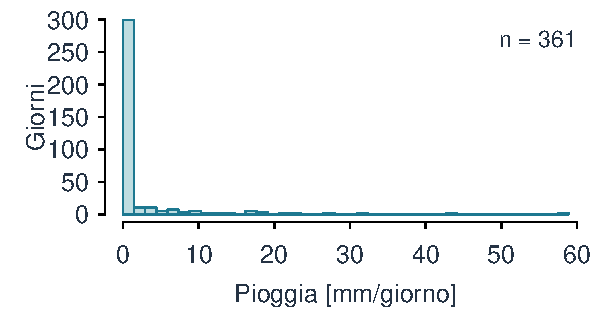
\includegraphics[width=\linewidth,height=5.0cm,keepaspectratio]{hist_pioggia_2024.pdf}
\PBody{Molti giorni asciutti e pochi eventi intensi producono una coda verso destra.}
\end{minipage}\hfill
\begin{minipage}[t]{8.8cm}
\PLabel{Logaritmo con riferimento di 1 mm}
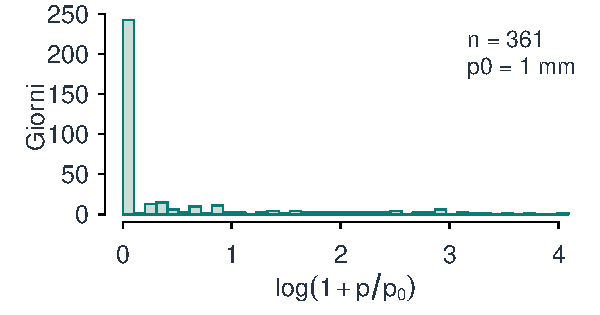
\includegraphics[width=\linewidth,height=5.0cm,keepaspectratio]{hist_pioggia_log1p_2024.pdf}
\PBody{$u=\ln(1+p/p_0)$, con $p_0=1\,\mathrm{mm}$. La frequenza conta ancora giorni.}
\end{minipage}
\vspace{2mm}\PSmall{Roma/Ciampino 2024, Meteostat: 361 giorni con pioggia disponibile, incluse stime di modello. La notazione abbreviata \texttt{log1p(pioggia)} assume che i valori numerici della pioggia siano espressi in millimetri.}

\end{minipage}%
\end{lrbox}
\typeout{FULLBOX:069:W:\the\ht\FullWideBox:\the\dp\FullWideBox}
\begin{frame}[plain]\hypertarget{slide69}{}
\bookmark[level=1,page=69]{Precipitazioni: leggere la stessa serie su due scale}
\begin{tikzpicture}[remember picture,overlay]
\PilotChrome{Precipitazioni: leggere la stessa serie su due scale}{TRASFORMAZIONI}{69}{Una trasformazione logaritmica conserva gli zeri e comprime i valori elevati; le distanze lungo l’asse cambiano significato.}
\node[anchor=north west,inner sep=0] at ([xshift=0.96cm,yshift=-2.13cm]current page.north west) {\usebox{\FullWideBox}};
\end{tikzpicture}
\end{frame}

% SLIDE 070 | Z-score: cambia la scala, resta la forma | REVISIONE COMPLETA
\begin{lrbox}{\FullWideBox}%
\begin{minipage}[t]{18.1cm}\raggedright\color{Ink}\fontsize{11.3}{14.8}\selectfont

\begin{minipage}[t]{8.8cm}
\PLabel{Temperatura in gradi Celsius}
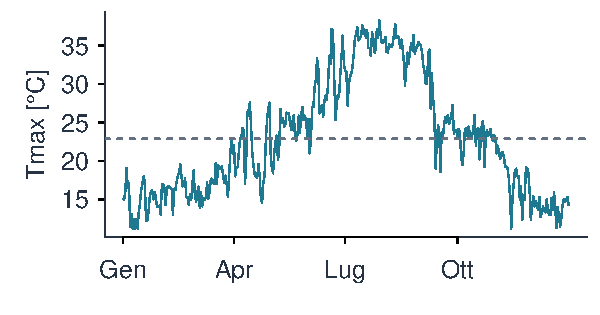
\includegraphics[width=\linewidth,height=5.0cm,keepaspectratio]{tmax_raw_2024.pdf}
\PBody{$\bar T=22{,}89\,{}^\circ\mathrm C$ e $s_T=7{,}55\,{}^\circ\mathrm C$, calcolati sui 366 giorni del 2024.}
\end{minipage}\hfill
\begin{minipage}[t]{8.8cm}
\PLabel{Scarti in deviazioni standard}
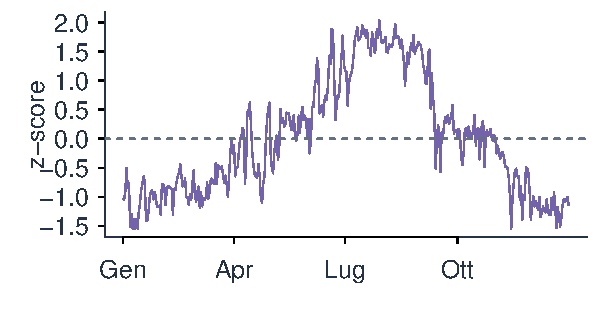
\includegraphics[width=\linewidth,height=5.0cm,keepaspectratio]{zscore_tmax_2024.pdf}
\PBody{$z_t=(T_t-\bar T)/s_T$: date e ordinamento dei valori rimangono gli stessi.}
\end{minipage}
\vspace{2mm}\PSmall{Roma/Ciampino 2024, Meteostat, incluse stime di modello. Si usano tutti i 366 giorni; sullo stesso campione $\bar z=0$ e $s_z=1$, salvo arrotondamenti.}

\end{minipage}%
\end{lrbox}
\typeout{FULLBOX:070:W:\the\ht\FullWideBox:\the\dp\FullWideBox}
\begin{frame}[plain]\hypertarget{slide70}{}
\bookmark[level=1,page=70]{Z-score: cambia la scala, resta la forma}
\begin{tikzpicture}[remember picture,overlay]
\PilotChrome{Z-score: cambia la scala, resta la forma}{TRASFORMAZIONI}{70}{Uno z-score positivo indica un valore sopra la media del riferimento scelto. La standardizzazione conserva la forma della serie.}
\node[anchor=north west,inner sep=0] at ([xshift=0.96cm,yshift=-2.13cm]current page.north west) {\usebox{\FullWideBox}};
\end{tikzpicture}
\end{frame}

% SLIDE 071 | Una serie temporale contiene più componenti | REVISIONE COMPLETA
\begin{lrbox}{\PilotLeftBox}%
\begin{minipage}[t]{10.05cm}\raggedright\color{Ink}\fontsize{11.3}{14.8}\selectfont

\[Y_t=T_t+S_t+E_t\]
\begin{tikzpicture}[x=1cm,y=1cm]
\foreach \yy/\lab in {3.7/tendenza,2.2/stagione,.7/residuo}{\draw[Rule](1.7,\yy)--(8.9,\yy);\node[pNote,anchor=east]at(1.5,\yy){\lab};}
\draw[GeoA,line width=1.2pt](1.8,3.4)--(8.6,4.05);
\draw[GeoB,line width=1.2pt,domain=1.8:8.6,samples=90]plot(\x,{2.2+.43*sin((\x-1.8)*160)});
\draw[GeoC,line width=.8pt]plot coordinates{(1.8,.65)(2.1,.9)(2.4,.55)(2.7,.7)(3,.95)(3.3,.35)(3.6,.8)(3.9,.6)(4.2,.95)(4.5,.6)(4.8,.7)(5.1,.4)(5.4,.85)(5.7,.65)(6,.8)(6.3,.55)(6.6,.9)(6.9,.6)(7.2,.7)(7.5,.95)(7.8,.55)(8.1,.8)(8.6,.6)};
\node[pNote,anchor=west]at(1.8,4.65){Schema additivo, componenti nella stessa unità};
\end{tikzpicture}
\PSmall{$t$ identifica il tempo; $T_t$ la tendenza, $S_t$ la componente periodica, $E_t$ il resto. La scomposizione dipende dal metodo e dalle ipotesi adottate.}

\end{minipage}%
\end{lrbox}
\typeout{FULLBOX:071:L:\the\ht\PilotLeftBox:\the\dp\PilotLeftBox}
\begin{lrbox}{\PilotRightBox}%
\begin{minipage}[t]{7.55cm}\raggedright\color{Ink}\fontsize{11.3}{14.8}\selectfont
\PCode{R · scomporre le medie mensili}{71_componenti.R}
\PSmall{\texttt{ts()} dichiara 12 valori per anno. \texttt{periodic} impone una stagione uguale negli anni.}
\PSmall{Servono mesi regolari e completi: qui si usano i 36 mesi simulati del 2022--2024.}
\end{minipage}%
\end{lrbox}
\typeout{FULLBOX:071:R:\the\ht\PilotRightBox:\the\dp\PilotRightBox}
\begin{frame}[plain]\hypertarget{slide71}{}
\bookmark[level=1,page=71]{Una serie temporale contiene più componenti}
\begin{tikzpicture}[remember picture,overlay]
\PilotChrome{Una serie temporale contiene più componenti}{SERIE TEMPORALI}{71}{La scomposizione descrive componenti della serie; l’attribuzione fisica di una variazione richiede informazioni ulteriori.}
\node[anchor=north west,inner sep=0] at ([xshift=0.96cm,yshift=-2.13cm]current page.north west) {\usebox{\PilotLeftBox}};
\node[anchor=north west,inner sep=0] at ([xshift=11.52cm,yshift=-2.13cm]current page.north west) {\usebox{\PilotRightBox}};
\end{tikzpicture}
\end{frame}

% SLIDE 072 | Ogni scarto dipende dal periodo di riferimento | REVISIONE COMPLETA
\begin{lrbox}{\PilotLeftBox}%
\begin{minipage}[t]{10.05cm}\raggedright\color{Ink}\fontsize{11.3}{14.8}\selectfont

\PLabel{Separare base di confronto e periodo esaminato}
\begin{tikzpicture}[x=1cm,y=1cm]
\fill[GeoA!15](.4,2.7)rectangle(6,3.65);
\fill[GeoB!20](6.1,2.7)rectangle(8.9,3.65);
\node[pLabel]at(1.8,3.15){2022};\node[pLabel]at(4.6,3.15){2023};\node[pLabel]at(7.5,3.15){2024};
\draw[GeoA,line width=1pt](.4,2.5)--(6,2.5);\node[pNote,below]at(3.2,2.45){base $B$ nell'esempio};
\draw[pEdge](3.2,1.8)--(3.2,.95)--(7.5,.95)--(7.5,2.45);
\node[pNote,anchor=north,text width=5.5cm]at(5.3,.65){una media di riferimento per ciascun mese};
\end{tikzpicture}
\[a_t=T_t-\bar T_{m(t),B}\]
\PSmall{$m(t)$ è il mese del giorno $t$; $\bar T_{m(t),B}$ è la media di quel mese nella base $B$. Nell'esempio la base di due anni ha solo scopo didattico.}

\end{minipage}%
\end{lrbox}
\typeout{FULLBOX:072:L:\the\ht\PilotLeftBox:\the\dp\PilotLeftBox}
\begin{lrbox}{\PilotRightBox}%
\begin{minipage}[t]{7.55cm}\raggedright\color{Ink}\fontsize{11.3}{14.8}\selectfont
\PCode{R · sottrarre il riferimento mensile}{72_riferimento.R}
\PSmall{\texttt{rif[mese]} abbina ogni giorno alla media del proprio mese, usando i nomi \texttt{01}, \ldots, \texttt{12}.}
\PSmall{Questa base breve ha scopo didattico; una normale climatica richiede un riferimento trentennale appropriato.}
\end{minipage}%
\end{lrbox}
\typeout{FULLBOX:072:R:\the\ht\PilotRightBox:\the\dp\PilotRightBox}
\begin{frame}[plain]\hypertarget{slide72}{}
\bookmark[level=1,page=72]{Ogni scarto dipende dal periodo di riferimento}
\begin{tikzpicture}[remember picture,overlay]
\PilotChrome{Ogni scarto dipende dal periodo di riferimento}{SERIE TEMPORALI}{72}{Il risultato va accompagnato dalla variabile, dal metodo di calcolo e dalle date del periodo di riferimento.}
\node[anchor=north west,inner sep=0] at ([xshift=0.96cm,yshift=-2.13cm]current page.north west) {\usebox{\PilotLeftBox}};
\node[anchor=north west,inner sep=0] at ([xshift=11.52cm,yshift=-2.13cm]current page.north west) {\usebox{\PilotRightBox}};
\end{tikzpicture}
\end{frame}

% SLIDE 073 | Precipitazioni per mese: confrontare distribuzioni | REVISIONE COMPLETA
\begin{lrbox}{\PilotLeftBox}%
\begin{minipage}[t]{10.05cm}\raggedright\color{Ink}\fontsize{11.3}{14.8}\selectfont

\PLabel{Meteostat · giorni disponibili nel 2019--2024}
\begin{center}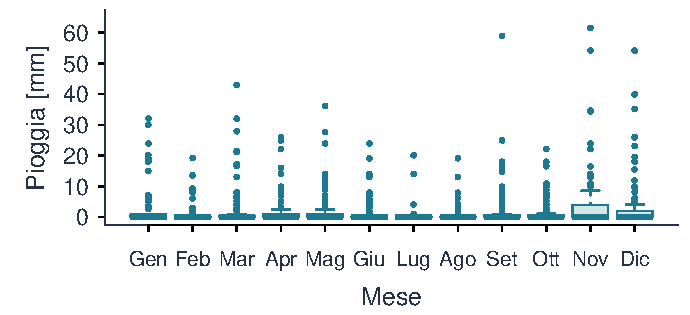
\includegraphics[width=\linewidth,height=4.8cm,keepaspectratio]{seasonality_prcp_box.pdf}\end{center}
\PSmall{I box raggruppano i giorni per mese. La copertura della pioggia varia fra gli anni e nel 2019 è assente. Fonte: Meteostat, incluse stime di modello.}

\end{minipage}%
\end{lrbox}
\typeout{FULLBOX:073:L:\the\ht\PilotLeftBox:\the\dp\PilotLeftBox}
\begin{lrbox}{\PilotRightBox}%
\begin{minipage}[t]{7.55cm}\raggedright\color{Ink}\fontsize{11.3}{14.8}\selectfont
\PCode{Prova su dati simulati}{73_boxplot_mese.R}
\PSmall{\texttt{factor()} fissa gruppi e ordine; \texttt{table()} conta le osservazioni per mese.}
\PSmall{Anni con copertura diversa contribuiscono in modo disuguale. Una mediana nulla può dipendere da molti giorni asciutti.}
\end{minipage}%
\end{lrbox}
\typeout{FULLBOX:073:R:\the\ht\PilotRightBox:\the\dp\PilotRightBox}
\begin{frame}[plain]\hypertarget{slide73}{}
\bookmark[level=1,page=73]{Precipitazioni per mese: confrontare distribuzioni}
\begin{tikzpicture}[remember picture,overlay]
\PilotChrome{Precipitazioni per mese: confrontare distribuzioni}{SERIE TEMPORALI}{73}{I boxplot mensili confrontano distribuzioni di valori giornalieri; i totali mensili e annui rispondono a domande differenti.}
\node[anchor=north west,inner sep=0] at ([xshift=0.96cm,yshift=-2.13cm]current page.north west) {\usebox{\PilotLeftBox}};
\node[anchor=north west,inner sep=0] at ([xshift=11.52cm,yshift=-2.13cm]current page.north west) {\usebox{\PilotRightBox}};
\end{tikzpicture}
\end{frame}

% SLIDE 074 | Precipitazione annua e copertura dei dati | REVISIONE COMPLETA
\begin{lrbox}{\PilotLeftBox}%
\begin{minipage}[t]{10.05cm}\raggedright\color{Ink}\fontsize{11.3}{14.8}\selectfont

\PLabel{Somme dei giorni disponibili · 2020--2024}
\begin{center}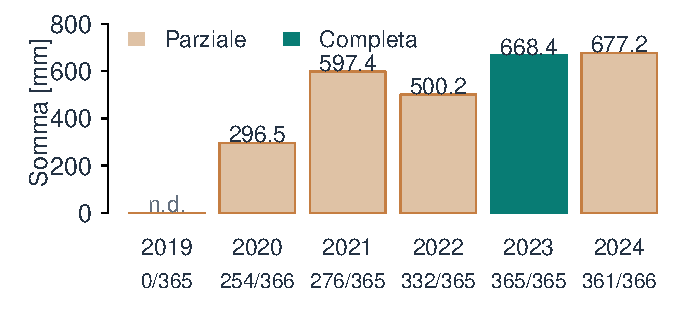
\includegraphics[width=\linewidth,height=4.7cm,keepaspectratio]{annual_prcp_totals.pdf}\end{center}
\PSmall{Le barre mostrano somme parziali quando mancano giorni. Il 2019 è privo di dati. Fonte: Meteostat, incluse stime di modello.}

\end{minipage}%
\end{lrbox}
\typeout{FULLBOX:074:L:\the\ht\PilotLeftBox:\the\dp\PilotLeftBox}
\begin{lrbox}{\PilotRightBox}%
\begin{minipage}[t]{7.55cm}\raggedright\color{Ink}\fontsize{11.3}{14.8}\selectfont

\PCode{Prova su dati simulati}{74_totali_annui.R}
\PSmall{Per dati incompleti: $S_y=\sum_{t\in O_y}p_t$ e $c_y=n_y/N_y$. $O_y$ raccoglie i giorni validi, $n_y=|O_y|$, $N_y$ i giorni attesi.}
\PSmall{Nei dati simulati $c_y=1$. \texttt{na.rm=TRUE} da solo non risolve il problema della copertura incompleta.}

\end{minipage}%
\end{lrbox}
\typeout{FULLBOX:074:R:\the\ht\PilotRightBox:\the\dp\PilotRightBox}
\begin{frame}[plain]\hypertarget{slide74}{}
\bookmark[level=1,page=74]{Precipitazione annua e copertura dei dati}
\begin{tikzpicture}[remember picture,overlay]
\PilotChrome{Precipitazione annua e copertura dei dati}{SERIE TEMPORALI}{74}{Confrontare le somme insieme alla copertura; una somma di giorni disponibili può sottostimare il totale dell’anno.}
\node[anchor=north west,inner sep=0] at ([xshift=0.96cm,yshift=-2.13cm]current page.north west) {\usebox{\PilotLeftBox}};
\node[anchor=north west,inner sep=0] at ([xshift=11.52cm,yshift=-2.13cm]current page.north west) {\usebox{\PilotRightBox}};
\end{tikzpicture}
\end{frame}

% SLIDE 075 | Risoluzione e durata limitano ciò che si osserva | REVISIONE COMPLETA
\begin{lrbox}{\PilotLeftBox}%
\begin{minipage}[t]{10.05cm}\raggedright\color{Ink}\fontsize{11.3}{14.8}\selectfont

\PLabel{Un evento breve può cadere fra due letture}
\begin{tikzpicture}[x=.88cm,y=1cm]
\draw[pAxis](0,.5)--(9,.5)node[right,pNote]{tempo};
\draw[pAxis](0,.5)--(0,4.1)node[above,pNote]{livello};
\draw[GeoA,line width=1.3pt]plot[smooth]coordinates{(.2,1)(1.5,1.1)(2.3,1)(3.0,1.2)(3.6,3.7)(4.0,1.5)(4.5,1.1)(6,1.0)(8.5,1.15)};
\foreach \xx/\yy in {.5/1.02,2.5/1.02,4.5/1.1,6.5/1.04,8.5/1.15}{\draw[GeoB,dashed](\xx,.5)--(\xx,\yy);\fill[GeoB](\xx,\yy)circle(2.8pt);}
\draw[GeoB,{Latex[length=1.7mm]}-{Latex[length=1.7mm]}](4.5,.05)--(6.5,.05);\node[pNote,below]at(5.5,.05){passo $\Delta t$};
\node[pNote,text width=3cm,anchor=west]at(4.3,3.2){picco non registrato\par dalle letture rade};
\end{tikzpicture}
\PBody{Il passo di acquisizione controlla i fenomeni brevi osservabili. La durata della serie controlla il numero di cicli e di anni che si possono confrontare.}

\end{minipage}%
\end{lrbox}
\typeout{FULLBOX:075:L:\the\ht\PilotLeftBox:\the\dp\PilotLeftBox}
\begin{lrbox}{\PilotRightBox}%
\begin{minipage}[t]{7.55cm}\raggedright\color{Ink}\fontsize{11.3}{14.8}\selectfont
\PCode{R · verificare la griglia giornaliera}{75_griglia_temporale.R}
\PSmall{\texttt{diff()} misura i passi; \texttt{seq()} costruisce il calendario atteso; \texttt{setdiff()} trova le date assenti.}
\PSmall{Un calendario completo può contenere misure \texttt{NA}: controllare anche i valori.}
\end{minipage}%
\end{lrbox}
\typeout{FULLBOX:075:R:\the\ht\PilotRightBox:\the\dp\PilotRightBox}
\begin{frame}[plain]\hypertarget{slide75}{}
\bookmark[level=1,page=75]{Risoluzione e durata limitano ciò che si osserva}
\begin{tikzpicture}[remember picture,overlay]
\PilotChrome{Risoluzione e durata limitano ciò che si osserva}{SERIE TEMPORALI}{75}{Annotare frequenza delle misure, durata, date assenti e cambi di protocollo; una serie numericamente continua può essere disomogenea.}
\node[anchor=north west,inner sep=0] at ([xshift=0.96cm,yshift=-2.13cm]current page.north west) {\usebox{\PilotLeftBox}};
\node[anchor=north west,inner sep=0] at ([xshift=11.52cm,yshift=-2.13cm]current page.north west) {\usebox{\PilotRightBox}};
\end{tikzpicture}
\end{frame}

% SLIDE 076 | Media e mediana mobile: quale finestra si usa? | REVISIONE COMPLETA
\begin{lrbox}{\PilotLeftBox}%
\begin{minipage}[t]{10.05cm}\raggedright\color{Ink}\fontsize{11.3}{14.8}\selectfont

\PLabel{Finestra centrata di ampiezza dispari}
\begin{tikzpicture}[x=.85cm,y=1cm]
\fill[GeoA!12](2.7,.4)rectangle(7.3,2.85);
\draw[pAxis](.2,.7)--(10,.7)node[right,pNote]{giorni};
\foreach \xx/\yy in {1/1.3,2/1.5,3/1.2,4/1.8,5/2.6,6/1.7,7/1.4,8/1.8,9/1.9}{\draw[Muted](\xx,.7)--(\xx,\yy);\fill[GeoA](\xx,\yy)circle(2.3pt);}
\node[pNote,below]at(3,.65){$t-h$};\node[pNote,below]at(5,.65){$t$};\node[pNote,below]at(7,.65){$t+h$};
\node[pNote]at(5,3.2){nell'esempio schematico: $h=2$, $k=5$};
\end{tikzpicture}
\[M_t=\frac{1}{2h+1}\sum_{j=-h}^{h}x_{t+j}\]
\PSmall{Nel codice $k=31$ e $h=15$. Il valore centrato usa osservazioni prima e dopo $t$; ai bordi la finestra completa non è disponibile.}

\end{minipage}%
\end{lrbox}
\typeout{FULLBOX:076:L:\the\ht\PilotLeftBox:\the\dp\PilotLeftBox}
\begin{lrbox}{\PilotRightBox}%
\begin{minipage}[t]{7.55cm}\raggedright\color{Ink}\fontsize{11.3}{14.8}\selectfont
\PCode{R · finestra di 31 giorni}{76_medie_mobili.R}
\PSmall{\texttt{rep(1/31,31)} crea pesi uguali. Si escludono i 15 giorni ai due estremi anche per la mediana.}
\PSmall{La mediana risente meno dei picchi isolati. Entrambe le curve centrate usano anche valori successivi al giorno rappresentato.}
\end{minipage}%
\end{lrbox}
\typeout{FULLBOX:076:R:\the\ht\PilotRightBox:\the\dp\PilotRightBox}
\begin{frame}[plain]\hypertarget{slide76}{}
\bookmark[level=1,page=76]{Media e mediana mobile: quale finestra si usa?}
\begin{tikzpicture}[remember picture,overlay]
\PilotChrome{Media e mediana mobile: quale finestra si usa?}{SERIE TEMPORALI}{76}{Dichiarare ampiezza, centratura, trattamento dei bordi e dei mancanti. Una finestra di k righe dura k giorni solo su una griglia giornaliera regolare.}
\node[anchor=north west,inner sep=0] at ([xshift=0.96cm,yshift=-2.13cm]current page.north west) {\usebox{\PilotLeftBox}};
\node[anchor=north west,inner sep=0] at ([xshift=11.52cm,yshift=-2.13cm]current page.north west) {\usebox{\PilotRightBox}};
\end{tikzpicture}
\end{frame}

% SLIDE 077 | LOESS: stimare una regressione vicino a ogni punto | REVISIONE COMPLETA
\begin{lrbox}{\PilotLeftBox}%
\begin{minipage}[t]{10.05cm}\raggedright\color{Ink}\fontsize{11.3}{14.8}\selectfont

\PLabel{Un intorno, pesi diversi, una stima locale}
\begin{tikzpicture}[x=.96cm,y=.8cm]
\fill[GeoA!10](2.0,.4)rectangle(7.5,3.9);
\draw[pAxis](.2,.4)--(9,.4)node[right,pNote]{$t$};
\draw[pAxis](.2,.4)--(.2,4.15)node[above,pNote]{$y$};
\draw[Classical,line width=1.2pt](2.1,1.2)--(7.4,2.8);
\foreach \xx/\yy/\rr in {.7/1/1.2,1.3/1.25/1.2,2.3/1.1/1.5,3.0/1.65/2.2,3.8/1.5/2.8,4.7/2.2/3.3,5.5/2.0/2.8,6.3/2.65/2.2,7.2/2.6/1.5,8.2/3/1.2}{\fill[GeoA](\xx,\yy)circle(\rr pt);}
\draw[GeoB,dashed](4.7,.4)--(4.7,3.6);\node[pNote,below]at(4.7,.35){$t_0$};
\node[pNote,text width=4cm]at(5.6,4.3){punti più vicini: peso maggiore};
\end{tikzpicture}
\[\min_{a,b}\sum_i w_i\bigl[y_i-a-b(t_i-t_0)\bigr]^2\]
\PSmall{Schema lineare locale: $\widehat y(t_0)=\widehat a$. I pesi $w_i(t_0)$ diminuiscono con la distanza; l'intorno cambia quando cambia $t_0$.}

\end{minipage}%
\end{lrbox}
\typeout{FULLBOX:077:L:\the\ht\PilotLeftBox:\the\dp\PilotLeftBox}
\begin{lrbox}{\PilotRightBox}%
\begin{minipage}[t]{7.55cm}\raggedright\color{Ink}\fontsize{11.3}{14.8}\selectfont
\PCode{R · LOESS di grado 1}{77_loess_locale.R}
\PSmall{\texttt{degree = 1} usa rette locali; \texttt{span = 0.2} usa circa il 20\% dei punti per intorno.}
\PSmall{Si possono usare polinomi quadratici e una procedura robusta, con \texttt{family = "symmetric"}.}
\end{minipage}%
\end{lrbox}
\typeout{FULLBOX:077:R:\the\ht\PilotRightBox:\the\dp\PilotRightBox}
\begin{frame}[plain]\hypertarget{slide77}{}
\bookmark[level=1,page=77]{LOESS: stimare una regressione vicino a ogni punto}
\begin{tikzpicture}[remember picture,overlay]
\PilotChrome{LOESS: stimare una regressione vicino a ogni punto}{SERIE TEMPORALI}{77}{LOESS combina regressioni locali; la frazione di punti e il grado del polinomio fanno parte della definizione della curva.}
\node[anchor=north west,inner sep=0] at ([xshift=0.96cm,yshift=-2.13cm]current page.north west) {\usebox{\PilotLeftBox}};
\node[anchor=north west,inner sep=0] at ([xshift=11.52cm,yshift=-2.13cm]current page.north west) {\usebox{\PilotRightBox}};
\end{tikzpicture}
\end{frame}

% SLIDE 078 | Il parametro span fissa una frazione di osservazioni | REVISIONE COMPLETA
\begin{lrbox}{\PilotLeftBox}%
\begin{minipage}[t]{10.05cm}\raggedright\color{Ink}\fontsize{11.3}{14.8}\selectfont

\PLabel{Stesso punto centrale, intorni differenti}
\begin{tikzpicture}[x=.9cm,y=1cm]
\fill[GeoA!15](4.15,2.15)rectangle(5.85,3.0);
\fill[GeoB!18](2.1,.45)rectangle(7.9,1.3);
\foreach \yy in {2.55,.85}{\draw[Rule](.5,\yy)--(9.5,\yy);\foreach \xx in {1,1.5,...,9}{\fill[Muted](\xx,\yy)circle(1.6pt);}}
\draw[Classical,dashed](5,.2)--(5,3.35);
\node[pNote,anchor=west]at(.5,3.65){span piccolo: intorno ristretto};
\node[pNote,anchor=west]at(.5,1.75){span grande: intorno esteso};
\node[pNote,below]at(5,.15){punto di stima $t_0$};
\end{tikzpicture}
\[k\simeq\alpha n,\qquad \alpha=\texttt{span}\quad(0<\alpha\leq1)\]
\PSmall{$k$ è il numero di punti vicini, $n$ la numerosità. Con date irregolari, la durata dell'intorno cambia anche a parità di $\alpha$.}

\end{minipage}%
\end{lrbox}
\typeout{FULLBOX:078:L:\the\ht\PilotLeftBox:\the\dp\PilotLeftBox}
\begin{lrbox}{\PilotRightBox}%
\begin{minipage}[t]{7.55cm}\raggedright\color{Ink}\fontsize{11.3}{14.8}\selectfont
\PCode{R · confrontare due valori di span}{78_confrontare_span.R}
\PSmall{\texttt{cbind()} affianca le curve; \texttt{matplot()} le disegna insieme. Intorni piccoli consentono variazioni rapide.}
\PSmall{Confrontare le curve con i dati; LOESS da solo non giustifica previsioni oltre le date osservate.}
\end{minipage}%
\end{lrbox}
\typeout{FULLBOX:078:R:\the\ht\PilotRightBox:\the\dp\PilotRightBox}
\begin{frame}[plain]\hypertarget{slide78}{}
\bookmark[level=1,page=78]{Il parametro span fissa una frazione di osservazioni}
\begin{tikzpicture}[remember picture,overlay]
\PilotChrome{Il parametro span fissa una frazione di osservazioni}{SERIE TEMPORALI}{78}{Span misura una frazione del campione, non una durata fissa in giorni. Dichiarare anche il grado e l’eventuale procedura robusta.}
\node[anchor=north west,inner sep=0] at ([xshift=0.96cm,yshift=-2.13cm]current page.north west) {\usebox{\PilotLeftBox}};
\node[anchor=north west,inner sep=0] at ([xshift=11.52cm,yshift=-2.13cm]current page.north west) {\usebox{\PilotRightBox}};
\end{tikzpicture}
\end{frame}

% SLIDE 079 | La figura deve mostrare dati, metodo e parametri | REVISIONE COMPLETA
\begin{lrbox}{\PilotLeftBox}%
\begin{minipage}[t]{10.05cm}\raggedright\color{Ink}\fontsize{11.3}{14.8}\selectfont

\PLabel{Un esempio di legenda verificabile}
\begin{tikzpicture}[x=.95cm,y=1cm]
\draw[pAxis](.3,.5)--(9,.5)node[right,pNote]{tempo};
\draw[pAxis](.3,.5)--(.3,4.4)node[above,pNote]{$T$};
\draw[Muted!55,line width=.8pt]plot coordinates{(.6,1.5)(1,2.2)(1.4,1.7)(1.8,2.8)(2.2,2.4)(2.6,3.6)(3,2.7)(3.4,3.4)(3.8,2.3)(4.2,2.7)(4.6,1.9)(5,2.2)(5.4,1.0)(5.8,1.6)(6.2,.9)(6.6,1.4)(7,1.1)(7.4,2.1)(7.8,1.8)(8.3,2.5)};
\draw[GeoA,line width=1.6pt]plot[smooth]coordinates{(1,1.9)(2,2.6)(3,3)(4,2.6)(5,1.8)(6,1.3)(7,1.5)(8,2.1)};
\draw[Muted!60,line width=1pt](1.1,4.5)--(1.8,4.5);\node[pNote,anchor=west]at(1.9,4.5){dati originali};
\draw[GeoA,line width=1.6pt](4.8,4.5)--(5.5,4.5);\node[pNote,anchor=west]at(5.6,4.5){media mobile 31 g};
\end{tikzpicture}
\PBody{Nel testo della figura dichiarare: finestra centrata, estremi esclusi, unità, periodo e provenienza dei dati. Lo schema mostra perché conservare visibili le oscillazioni originali.}

\end{minipage}%
\end{lrbox}
\typeout{FULLBOX:079:L:\the\ht\PilotLeftBox:\the\dp\PilotLeftBox}
\begin{lrbox}{\PilotRightBox}%
\begin{minipage}[t]{7.55cm}\raggedright\color{Ink}\fontsize{11.3}{14.8}\selectfont

\PCode{R · osservazioni e media mobile}{79_documentare_curva.R}
\PSmall{\texttt{lines()} aggiunge una curva al grafico aperto; \texttt{legend()} specifica a quale serie corrisponde ogni colore. Esempio su dati simulati.}

\end{minipage}%
\end{lrbox}
\typeout{FULLBOX:079:R:\the\ht\PilotRightBox:\the\dp\PilotRightBox}
\begin{frame}[plain]\hypertarget{slide79}{}
\bookmark[level=1,page=79]{La figura deve mostrare dati, metodo e parametri}
\begin{tikzpicture}[remember picture,overlay]
\PilotChrome{La figura deve mostrare dati, metodo e parametri}{SERIE TEMPORALI}{79}{La curva riassume le osservazioni e va accompagnata dalle informazioni necessarie per ricostruirla.}
\node[anchor=north west,inner sep=0] at ([xshift=0.96cm,yshift=-2.13cm]current page.north west) {\usebox{\PilotLeftBox}};
\node[anchor=north west,inner sep=0] at ([xshift=11.52cm,yshift=-2.13cm]current page.north west) {\usebox{\PilotRightBox}};
\end{tikzpicture}
\end{frame}

% SLIDE 080 | Confrontare smussamenti con scale differenti | REVISIONE COMPLETA
\begin{lrbox}{\PilotLeftBox}%
\begin{minipage}[t]{10.05cm}\raggedright\color{Ink}\fontsize{11.3}{14.8}\selectfont

\PLabel{Roma/Ciampino · 2019--2024 · 2192 giorni}
\begin{center}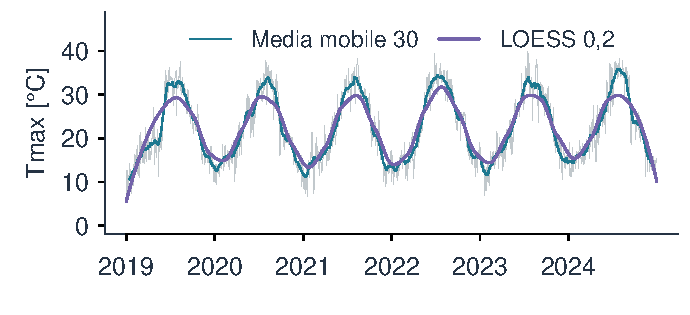
\includegraphics[width=\linewidth,height=4.8cm,keepaspectratio]{trend_smoothing_tmax.pdf}\end{center}
\PSmall{Serie giornaliera, media mobile di 30 giorni e LOESS con span $0{,}2$, grado 2. La media usa $t-14,\ldots,t+15$. Fonte: Meteostat, incluse stime di modello.}

\end{minipage}%
\end{lrbox}
\typeout{FULLBOX:080:L:\the\ht\PilotLeftBox:\the\dp\PilotLeftBox}
\begin{lrbox}{\PilotRightBox}%
\begin{minipage}[t]{7.55cm}\raggedright\color{Ink}\fontsize{11.3}{14.8}\selectfont

\PCode{Prova su dati simulati}{80_scale_smussamento.R}
\PBody{Nel file didattico ci sono 1096 giorni. Una finestra di 31 giorni e LOESS con span $0{,}2$ usano numerosità molto diverse.}
\PInfo{Nella figura originale la media è su 30 giorni; negli esempi R si usano 31 giorni per avere una finestra centrata simmetrica.}

\end{minipage}%
\end{lrbox}
\typeout{FULLBOX:080:R:\the\ht\PilotRightBox:\the\dp\PilotRightBox}
\begin{frame}[plain]\hypertarget{slide80}{}
\bookmark[level=1,page=80]{Confrontare smussamenti con scale differenti}
\begin{tikzpicture}[remember picture,overlay]
\PilotChrome{Confrontare smussamenti con scale differenti}{SERIE TEMPORALI}{80}{Prima di confrontare due curve, confrontare la quantità di dati che ciascuna usa localmente e il trattamento degli estremi.}
\node[anchor=north west,inner sep=0] at ([xshift=0.96cm,yshift=-2.13cm]current page.north west) {\usebox{\PilotLeftBox}};
\node[anchor=north west,inner sep=0] at ([xshift=11.52cm,yshift=-2.13cm]current page.north west) {\usebox{\PilotRightBox}};
\end{tikzpicture}
\end{frame}

% SLIDE 081 | Scarti rispetto alla media mensile del campione | REVISIONE COMPLETA
\begin{lrbox}{\PilotLeftBox}%
\begin{minipage}[t]{10.05cm}\raggedright\color{Ink}\fontsize{11.3}{14.8}\selectfont

\PLabel{Riferimento mensile: il campione 2019--2024}
\begin{center}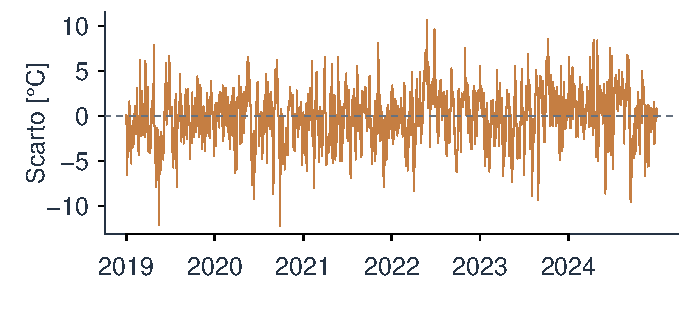
\includegraphics[width=\linewidth,height=4.6cm,keepaspectratio]{anomalies_tmax.pdf}\end{center}
\PSmall{Ogni giorno è confrontato con la media del proprio mese sul campione di 2192 temperature. Gli scarti usano il riferimento 2019--2024. Fonte: Meteostat, incluse stime di modello.}

\end{minipage}%
\end{lrbox}
\typeout{FULLBOX:081:L:\the\ht\PilotLeftBox:\the\dp\PilotLeftBox}
\begin{lrbox}{\PilotRightBox}%
\begin{minipage}[t]{7.55cm}\raggedright\color{Ink}\fontsize{11.3}{14.8}\selectfont
\PCode{Prova su dati simulati}{81_scarti_mensili.R}
\PSmall{$a_t=T_t-\bar T_{m(t)}$: scarti positivi indicano temperature sopra la media del mese. Sullo stesso campione gli scarti medi mensili sono nulli.}
\PSmall{Il codice usa la base simulata 2022--2024; cambiando la base cambiano gli scarti.}
\end{minipage}%
\end{lrbox}
\typeout{FULLBOX:081:R:\the\ht\PilotRightBox:\the\dp\PilotRightBox}
\begin{frame}[plain]\hypertarget{slide81}{}
\bookmark[level=1,page=81]{Scarti rispetto alla media mensile del campione}
\begin{tikzpicture}[remember picture,overlay]
\PilotChrome{Scarti rispetto alla media mensile del campione}{SERIE TEMPORALI}{81}{Chiamare questi valori scarti rispetto al campione e dichiarare gli anni usati; una normale climatica richiede un riferimento adeguato.}
\node[anchor=north west,inner sep=0] at ([xshift=0.96cm,yshift=-2.13cm]current page.north west) {\usebox{\PilotLeftBox}};
\node[anchor=north west,inner sep=0] at ([xshift=11.52cm,yshift=-2.13cm]current page.north west) {\usebox{\PilotRightBox}};
\end{tikzpicture}
\end{frame}

% SLIDE 082 | Smussare una serie con un salto strumentale | REVISIONE COMPLETA
\begin{lrbox}{\PilotLeftBox}%
\begin{minipage}[t]{10.05cm}\raggedright\color{Ink}\fontsize{11.3}{14.8}\selectfont

\PLabel{Salto artificiale su una serie Meteostat}
\begin{center}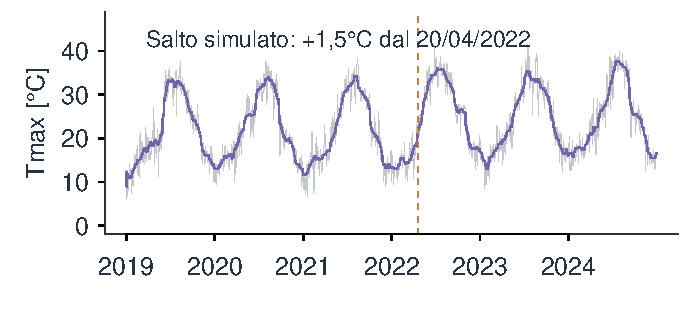
\includegraphics[width=\linewidth,height=4.6cm,keepaspectratio]{discontinuity_demo.pdf}\end{center}
\PSmall{Nel grafico: $+1{,}5\,{}^\circ\mathrm C$ dal 20 aprile 2022 e mediana mobile di 31 giorni. La curva conserva il cambio di livello. Fonte: Meteostat, incluse stime di modello; salto aggiunto.}

\end{minipage}%
\end{lrbox}
\typeout{FULLBOX:082:L:\the\ht\PilotLeftBox:\the\dp\PilotLeftBox}
\begin{lrbox}{\PilotRightBox}%
\begin{minipage}[t]{7.55cm}\raggedright\color{Ink}\fontsize{11.3}{14.8}\selectfont
\PCode{R · altro esempio simulato}{82_salto_strumento.R}
\PSmall{$Y_t=X_t+\delta\,\mathbf1\{t\geq t_0\}$: da $t_0$ si aggiunge $\delta=2\,{}^\circ\mathrm C$. La condizione logica vale 0 prima e 1 dopo il cambio.}
\PSmall{L'attribuzione a uno strumento richiede metadati e misure indipendenti.}
\end{minipage}%
\end{lrbox}
\typeout{FULLBOX:082:R:\the\ht\PilotRightBox:\the\dp\PilotRightBox}
\begin{frame}[plain]\hypertarget{slide82}{}
\bookmark[level=1,page=82]{Smussare una serie con un salto strumentale}
\begin{tikzpicture}[remember picture,overlay]
\PilotChrome{Smussare una serie con un salto strumentale}{SERIE TEMPORALI}{82}{Un cambiamento del sistema di misura può imitare un cambiamento ambientale; la curva smussata da sola non distingue le due cause.}
\node[anchor=north west,inner sep=0] at ([xshift=0.96cm,yshift=-2.13cm]current page.north west) {\usebox{\PilotLeftBox}};
\node[anchor=north west,inner sep=0] at ([xshift=11.52cm,yshift=-2.13cm]current page.north west) {\usebox{\PilotRightBox}};
\end{tikzpicture}
\end{frame}

% SLIDE 083 | Descrivere una serie e verificare una previsione | REVISIONE COMPLETA
\begin{lrbox}{\PilotLeftBox}%
\begin{minipage}[t]{10.05cm}\raggedright\color{Ink}\fontsize{11.3}{14.8}\selectfont

\PLabel{I dati futuri vanno tenuti fuori dalla stima}
\begin{tikzpicture}[x=1cm,y=1cm]
\fill[GeoA!15](.4,2.4)rectangle(5.8,3.65);
\fill[GeoB!18](5.9,2.4)rectangle(9,3.65);
\node[pLabel,text width=5cm]at(3.1,3.0){addestramento\par 2022--2023};
\node[pLabel,text width=2.8cm]at(7.45,3.0){valutazione\par 2024};
\draw[pAxis](.4,1.9)--(9,1.9)node[right,pNote]{tempo};
\draw[GeoB,dashed,line width=1pt](5.85,1.4)--(5.85,4.15);
\node[pNote,text width=4cm]at(3.1,.8){stimare parametri e scegliere il metodo};
\node[pNote,text width=3cm]at(7.45,.8){confrontare previsioni e valori successivi};
\end{tikzpicture}
\PBody{Una media centrata usa anche dati successivi al giorno che rappresenta. Applicarla prima di una valutazione predittiva può trasferire informazione dal futuro al passato.}

\end{minipage}%
\end{lrbox}
\typeout{FULLBOX:083:L:\the\ht\PilotLeftBox:\the\dp\PilotLeftBox}
\begin{lrbox}{\PilotRightBox}%
\begin{minipage}[t]{7.55cm}\raggedright\color{Ink}\fontsize{11.3}{14.8}\selectfont
\PCode{R · riservare un periodo di controllo}{83_validazione_tempo.R}
\PSmall{Anche standardizzazione, parametri e imputazione si stimano sul periodo di addestramento.}
\PSmall{Dividere casualmente giorni vicini può rendere la verifica troppo favorevole quando i dati sono dipendenti nel tempo.}
\end{minipage}%
\end{lrbox}
\typeout{FULLBOX:083:R:\the\ht\PilotRightBox:\the\dp\PilotRightBox}
\begin{frame}[plain]\hypertarget{slide83}{}
\bookmark[level=1,page=83]{Descrivere una serie e verificare una previsione}
\begin{tikzpicture}[remember picture,overlay]
\PilotChrome{Descrivere una serie e verificare una previsione}{SERIE TEMPORALI}{83}{Uno smussamento descrittivo non è una previsione. Per valutare capacità predittiva, rispettare l’ordine temporale e tenere separati i dati di verifica.}
\node[anchor=north west,inner sep=0] at ([xshift=0.96cm,yshift=-2.13cm]current page.north west) {\usebox{\PilotLeftBox}};
\node[anchor=north west,inner sep=0] at ([xshift=11.52cm,yshift=-2.13cm]current page.north west) {\usebox{\PilotRightBox}};
\end{tikzpicture}
\end{frame}

% SLIDE 084 | Domanda, dati e procedura nella conclusione | REVISIONE COMPLETA
\begin{lrbox}{\PilotLeftBox}%
\begin{minipage}[t]{10.05cm}\raggedright\color{Ink}\fontsize{11.3}{14.8}\selectfont

\PLabel{Ogni affermazione deve poter essere ricostruita}
\begin{tikzpicture}[x=1cm,y=1cm]
\node[pFlow,text width=3.7cm,minimum height=1.3cm](q)at(2.1,4){domanda\par quantità di interesse};
\node[pFlow,text width=3.7cm,minimum height=1.3cm](d)at(7,4){dati\par unità, origine, copertura};
\node[pFlow,text width=3.7cm,minimum height=1.3cm](m)at(2.1,1.5){procedura\par codice, parametri, ipotesi};
\node[pFlow,text width=3.7cm,minimum height=1.3cm](r)at(7,1.5){risultato\par stima, incertezza, limiti};
\draw[pEdge](q.south)--(m.north);\draw[pEdge](d.south)--(r.north);
\draw[pEdge](m.east)--(r.west);\draw[pEdge](q.east)--(d.west);
\end{tikzpicture}
\PBody{Per Terra01, specificare se si vuole la media delle misure o delle stazioni. Riportare numerosità, unità, pesi e differenza fra risultato simulato e valore atteso.}

\end{minipage}%
\end{lrbox}
\typeout{FULLBOX:084:L:\the\ht\PilotLeftBox:\the\dp\PilotLeftBox}
\begin{lrbox}{\PilotRightBox}%
\begin{minipage}[t]{7.55cm}\raggedright\color{Ink}\fontsize{11.3}{14.8}\selectfont
\PCode{R · conservare sintesi e versioni}{84_salvare_risultato.R}
\PSmall{\texttt{write.csv()} esporta la tabella; \texttt{sessionInfo()} registra R e pacchetti. Conservare anche dati iniziali e script.}
\PSmall{Il file accompagna una frase che definisce significato scientifico e ambito del risultato.}
\end{minipage}%
\end{lrbox}
\typeout{FULLBOX:084:R:\the\ht\PilotRightBox:\the\dp\PilotRightBox}
\begin{frame}[plain]\hypertarget{slide84}{}
\bookmark[level=1,page=84]{Domanda, dati e procedura nella conclusione}
\begin{tikzpicture}[remember picture,overlay]
\PilotChrome{Domanda, dati e procedura nella conclusione}{CONCLUSIONI}{84}{La conclusione deve rispondere alla domanda iniziale con la quantità corretta, usando dati e ipotesi dichiarati.}
\node[anchor=north west,inner sep=0] at ([xshift=0.96cm,yshift=-2.13cm]current page.north west) {\usebox{\PilotLeftBox}};
\node[anchor=north west,inner sep=0] at ([xshift=11.52cm,yshift=-2.13cm]current page.north west) {\usebox{\PilotRightBox}};
\end{tikzpicture}
\end{frame}

% SLIDE 085 | Riferimenti e materiali della lezione | REVISIONE COMPLETA
\begin{lrbox}{\PilotLeftBox}%
\begin{minipage}[t]{10.05cm}\raggedright\color{Ink}\fontsize{11.3}{14.8}\selectfont

\PLabel{Documentazione e approfondimenti}
\PBody{\href{https://www.r-project.org/}{R Project} e \href{https://cran.r-project.org/manuals.html}{manuali ufficiali}: linguaggio, importazione, funzioni e modelli.\\[3mm]
\href{https://www.statlearning.com/}{James e altri, \emph{An Introduction to Statistical Learning}}: regressione, validazione e metodi statistici.\\[3mm]
\href{https://www.openintro.org/book/os/}{Diez, Barr e Çetinkaya-Rundel, \emph{OpenIntro Statistics}}: campionamento, stime e incertezza.\\[3mm]
\href{https://dev.meteostat.net/}{Meteostat}: documentazione della fonte meteorologica delle figure.}
\vspace{3mm}\PSmall{I riferimenti puntuali, le unità e la provenienza dei dati sono raccolti in \texttt{FONTI\_E\_NOTE.txt}.}

\end{minipage}%
\end{lrbox}
\typeout{FULLBOX:085:L:\the\ht\PilotLeftBox:\the\dp\PilotLeftBox}
\begin{lrbox}{\PilotRightBox}%
\begin{minipage}[t]{7.55cm}\raggedright\color{Ink}\fontsize{11.3}{14.8}\selectfont

\PLabel{Per svolgere gli esercizi}
\PBody{\href{https://marzione00.github.io/Lab_Geo/\#laboratorio/m01-estimando}{GeoStat Lab · Terra01}\\
\emph{Definire la quantità di interesse}.}
\vspace{3mm}\PCode{R · riprendere il lavoro}{85_materiali.R}
\PInfo{Il pacchetto contiene il sorgente LaTeX, le figure, i CSV, i frammenti R e due script completi. I dati meteorologici di \texttt{demo} sono simulati e distinti dalle figure osservate.}

\end{minipage}%
\end{lrbox}
\typeout{FULLBOX:085:R:\the\ht\PilotRightBox:\the\dp\PilotRightBox}



\end{document}
